% PAQUETES
\documentclass[a4paper, 10pt, onecolumn,journal]{ieeeconf}
\overrideIEEEmargins
\usepackage[utf8]{inputenc}
\usepackage[T1]{fontenc}
\usepackage[spanish]{babel} 
\usepackage{fancyhdr}
\usepackage{lastpage}
\usepackage{graphicx}
\usepackage{amsmath}
\usepackage{amssymb} % Para símbolos matemáticos adicionales
\usepackage{adjustbox}
\usepackage{cleveref}
\usepackage[none]{hyphenat}
\usepackage{array}
\usepackage{float}     % Para el modificador [H]
\usepackage{multirow}
\usepackage{textcomp}
\newcommand{\defeq}{\mathrel{\mathop:}=}
\newcolumntype{C}[1]{>{\centering\arraybackslash}m{#1}}
\renewcommand{\arraystretch}{1.5} % Ajusta este valor para más o menos espacio entre filas

%\graphicspath{{imágenes/}}
\usepackage[backend=biber,style=ieee]{biblatex}
\bibliography{references}

% Configuración del encabezado y el pie de página
\pagestyle{fancy}
\fancyhf{}

% Encabezado
\fancyhead[L]{UNCuyo -- Ing. Mecatrónica \\ Mendoza - Argentina}
\fancyhead[C]{\textbf{311 -- AUTOMÁTICA Y MÁQUINAS ELÉCTRICAS \\ PROYECTO GLOBAL INTEGRADOR}}
\fancyhead[R]{Año: 2024 \\ Alumnos: Borquez y Escobar\\Fecha: 28/06/2024}

% Pie de página
\fancyfoot[C]{Página \thepage\ de \pageref{LastPage}} % Muestra "Página x de xx"

% Línea en la parte superior del encabezado
\renewcommand{\headrulewidth}{0.4pt}

% Línea en la parte inferior del pie de página
\renewcommand{\footrulewidth}{0.4pt}

% TÍTULO
\title{\LARGE \bf
Proyecto Global Integrador: Control de Accionamiento de CA con
Motor Sincrónico de Imanes Permanentes
}

% AUTORES
\author{Borquez Juan y Escobar Matías}

% INICIO DEL DOCUMENTO
\begin{document}

\maketitle
\thispagestyle{empty}
\pagestyle{fancy}

% RESUMEN
\begin{abstract}
	Este trabajo presenta el modelado, simulación, diseño y análisis de desempeño de un sistema de control automático para un accionamiento electromecánico de cuatro cuadrantes. El sistema incluye una máquina sincrónica de imanes permanentes trifásica (PMSM), alimentada por un inversor trifásico desde una fuente de corriente continua (CC), y un reductor de velocidad planetario conectado a la carga mecánica. Se utilizan sensores de retroalimentación, incluyendo un sensor de posición en el eje del motor, tres sensores de corriente instántanea de fase en la salida del inversor al estator de la máquina y un sensor de temperatura del bobinado del estator.
	La estrategía de control es la de control vectorial de campo orientado y se presenta la simulación y análisis del sistema físico y del controlador en tiempo continuo y la posterior discretización del controlador.
	Se comparan distintas formas de modelar el sistema y se determinan los efectos de la variación de los parámetros en la estabilidad del sistema y el desempeño del controlador. Se simula el sistema físico individualmente y acoplado al controlador aplicando consignas consistentes y suaves.
	Se determina que el controlador obtenido tiene un buen desempeño para la aplicación requerida y es implementable en una situación real.
\end{abstract}

% INTRODUCCIÓN
\section{INTRODUCCIÓN}
Modelado, simulación, diseño y análisis de desempeño de un Sistema de Control Automático de Posición y Movimiento para un Accionamiento electromecánico de 4 cuadrantes, compuesto por: máquina eléctrica de corriente alterna (CA) trifásica sincrónica con excitación por imanes permanentes (PMSM), alimentada por inversor trifásico desde fuente de corriente continua (CC); reductor de velocidad de engranajes planetarios de salida hacia la carga mecánica; realimentación con 1 sensor de posición en el eje del motor, más 3 sensores de corriente instantánea de fases en la salida del inversor trifásico al estator de la máquina (PMSM) y 1 sensor de temperatura del bobinado de estator.

El desarrollo del trabajo contiene tres partes principales.
En la parte \ref{subsec: modelado, simulación y análisis del sistema físico} se lleva a cabo el modelado, análisis y simulación del sistema físico.
Se obtienen las ecuaciones que lo modelan, obteniéndose un modelo que es inherentemente no lineal. Luego se comparan tres modelos derivados, el modelo LTI (Linear Time Invariant), que
se obtiene al asumir una especificación en el estado del sistema, el LPV (Lineal de Parámetros Variables), que se obtiene por linealización Jacobiana alrededor de un punto de operación y 
el modelo no lineal linealizado por realimentación no lineal. Se compara de los mismos el comportamiento ante perturbaciones y entradas de control esperables. Se analizan características del modelo de la planta, siendo las principales
la establidad, la controlabilidad y la observabilidad y cómo cambian ante la variación de parámetros característicos del sistem físico real.

En la parte \ref{subsec: Diseño del controlador} se diseña el controlador en cascada comenzando por la compensación de todas las realimentaciones 
naturales del sistema físico para control directo de los estados del mismo y asumiendo primero el acceso a todas las variables de estado a través de sensores ideales y actuación a través de modulador de torque ideal. Luego se diseñan
los lazos de control interno de corrientes con polos pre-establecidos para obtener el modulador de tensión solo proporcional. Luego se diseña el controlador externo de posición tipo PID
con el método de sintonía serie y se comparan los polos de los lazos de control con los de la planta. A continuación se diseña un observador de Luemberger de estado reducido para obtener una medida precisa de la velocidad angular con poco ruido para realimentar al controlador.
A continuación se evalúa el seguimiento de consignas de posición y se compara el desempeño en términos de las magnitudes de las acciones de control necesarias cuando estas consignas se van suavizando. Finalmente se 
evalúa el comportamiento cuando los sensores y el modulador de tensión no son ideales, y se muestra cómo, para no perder desempeño en el control, estos deben cumplir prestaciones mínimas en cuanto al rango de frecuencias en que operan.

En la parte \ref{subsubsec: Controlador discretizado} se hace el análisis y la descretización del controlador y se determina la velocidad mínima necesaria del dispositivo de control en el que se implemente para poder como se espera.

% ECUACIONES
\newpage

% DESARROLLO - PRESENTACIÓN DEL PROBLEMA
\section{PRESENTACIÓN DEL PROBLEMA}
El problema bajo estudio se encuentra bien detallado en la guía de referencia (\cite{c1}), por lo que en esta sección se indican solo los aspectos más relevantes de cada parte del problema.

% Carga mecánica
\subsection{\textbf{Carga mecánica}}
Aplicación simplificada de referencia: control de movimiento de 1 eje (descentralizado) para articulación de brazo manipulador robótico elemental de un grado de libertad (1 g.d.l.) rotacional de eje horizontal sometido a la acción de la aceleración de gravedad (péndulo rígido actuado), con eje de rotación fijo a base en sistema de referencia inercial (\cref{brazo}); con parámetros equivalentes variables según sea la carga útil transportada en el extremo.

\begin{figure}[H]
    \centering
    \begin{adjustbox}{max width=0.5\columnwidth}
        \framebox{\parbox{\columnwidth}{
            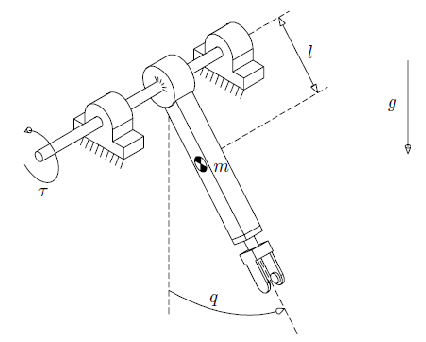
\includegraphics[width=\columnwidth]{1-Brazo.PNG}
        }}
    \end{adjustbox}
    \caption{Robot manipulador elemental de 1 g.d.l. en plano vertical (péndulo rígido actuado).}
    \label{brazo}
\end{figure}

% Caja reductora
\subsection{\textbf{Caja Reductora}}
Caja reductora reversible con sistema de engranajes planetarios, asumiendo acoplamiento rígido (sin elasticidad torsional y sin juego, holgura o ``backlash''); momento de inercia equivalente y pérdidas de energía por fricción interna, reflejados al eje de entrada y considerados junto con el motor.

% Máquina eléctrica PMSM
\subsection{\textbf{Máquina Eléctrica PMSM}}
Máquina eléctrica de CA trifásica sincrónica con excitación por imanes permanentes (PMSM) y estator conectado en estrella (simétrico y equilibrado) accesible en bornes de fases $abc$, con centro de estrella (punto “neutro”) flotante (no accesible).

% Subsistema térmico de la máquina eléctrica
\vspace*{0.1cm}
\subsubsection{\textbf{Subsistema térmico}} Modelo simplificado equivalente de primer orden, considerando sólo pérdidas
eléctricas resistivas por efecto Joule en bobinado de estator, despreciando pérdidas magnéticas
en el núcleo; transferencia de calor por conducción y convección natural, sin ventilación forzada.

% Inversor trifásico
\subsection{\textbf{Inversor trifásico de alimentación (modulador de tensión)}}

Inversor trifásico de 4 cuadrantes (regenerativo), consistente en puente trifásico con llaves electrónicas semiconductoras alimentado desde fuente de CC de tensión constante, conmutado con modulación de ancho de pulso.

No es parte de este proyecto el análisis del detalle de operación del inversor ni su fuente de energía de CC. Se considera al inversor trifásico y la fuente de CC como un Modulador idealizado de tensión trifásico (vectorial) (modelo promediado que se indica a continuación) para alimentación al estator de la Máquina Eléctrica.
\vspace*{0.1cm}
\subsubsection{\textbf{Modelo Promediado}}
Se considera un modelo promediado equivalente de tensiones sintetizadas de salida (componente fundamental, sin armónicos). Se trata de un sistema trifásico de tensiones de fase en bornes de estator, senoidales de secuencia positiva $abc$, equilibrado o balanceado, variable en Módulo $V_{sl}(t)$ y Frecuencia $\omega_e(t)$.

% SENSORES
\subsection{\textbf{Sensores de retroalimentación}}

El sistema cuenta con los siguientes dispositivos físicos y sus canales de medición y acondicionamiento:
\begin{itemize}
    \item 1 sensor de posición angular (codificador incremental o “encoder”) montado en el eje de motor, asumiendo proceso de “homming” y decodificación idealizados. Se logra la medición de la posición angular absoluta “rectificada” (al girar más de una revolución)
    \[\rightarrow \text{variable medida}: \theta_m(t)\]
    \item 3 sensores de corriente instantánea de fase, montados en salida trifásica del inversor hacia bornes del estator.
    \[\rightarrow \text{variables medidas}: i_{as}(t), i_{bs}(t), i_{cs}(t)\]
    \item 1 sensor de temperatura (ej. RTD) en bobinado de estator. Se mide la temperatura para monitoreo de calentamiento y estimación de resistencia de estator $R_s(t)$.
    \[\rightarrow \text{variable medida}: T_s^{\circ}(t)\]
\end{itemize}

% VARIABLES DE ESTADO UTILIZADAS EN EL MODELO
\subsection{\textbf{Variables principales en el Modelo Dinámico completo}}
Se utilizan las siguientes variables para representar el estado, las entradas y las salidas en el modelo del sistema dinámico completo.

\textbf{a) Excitaciones (entradas) externas:}
\begin{itemize}
    \item Variable manipulada (vectorial): Sistema trifásico de tensiones de fase reales en bornes de estator $v_{abcs}(t)$, con $V_{sl}(t)$ y $\omega_e(t)$ ajustables a través de manipulación de la modulación PWM del inversor.
    \item Variables de perturbación: Torque externo de carga mecánica $T_l(t)$ aplicado en la articulación del brazo manipulador. Temperatura ambiente $T_{amb}^{\circ}(t)$.
\end{itemize}

\textbf{b) Estado interno:}
\begin{itemize}
    \item Posición $\theta_m(t)$ y velocidad $\omega_m(t)$ en eje del motor. Corrientes virtuales equivalentes de estator $i_{qd0s}^r(t)$; temperatura de estator $T_s^{\circ}(t)$.
\end{itemize}

\textbf{c) Respuestas (salidas) externas:}
\begin{itemize}
    \item Variable controlada, no medida directamente (efector final): Posición angular de eje de la carga $q(t) \equiv \theta_l(t)$.
    \item Variables medidas (para realimentación): Posición angular de eje del motor $\theta_m(t)$. Sistema trifásico de corrientes de fase reales en bornes de estator $i_{abcs}(t)$. Temperatura de estator $T_s^{\circ}(t)$.
\end{itemize}


\section{ECUACIONES}
Se detallan en esta sección las ecuaciones que modelan las distintas partes del sistema, obtenidas de la guía de referencia (\cite{c1}), en la que también se detalla claramente el significado de cada uno de los términos en las ecuaciones.


\begin{itemize}
    % carga
    \item Modelo matemático simplificado equivalente no lineal de parámetros variables referido al eje de salida del tren de transmisión:
    \begin{equation}
        J_l \frac{d\omega_l(t)}{dt} = T_q(t) - b_l \omega_l(t) - T_l(t)
        \label{carga mecanica}
    \end{equation}
    \begin{equation}
        T_l(t) = k_l \sin(\theta_l(t)) + T_d(t)
        \label{torque de carga}
    \end{equation}
    \begin{equation}
        \frac{d\theta_l(t)}{dt} \equiv \omega_l(t) \Leftrightarrow \theta_l(t) = \int_{0}^{t} \omega_l(\zeta) \, d\zeta + \theta_l(0)
        \label{velocidad y posición de la carga}
    \end{equation}

    % transmisión
    \item Modelo equivalente rígido del tren de transmisión:
    \begin{equation}
        \omega_l(t) = \frac{1}{r} \cdot \omega_m(t)
        \label{relacion de velocidad en caja}
    \end{equation}
    \begin{equation}
        T_q(t) = r \cdot T_{dm}(t)
        \label{relacion de torque en caja}
    \end{equation}
    
    % sub-sistema mecánico PMSM
    \item Modelo matemático equivalente del sub-sistema mecánico de la máquina eléctrica:
    \begin{equation}
        J_m \frac{d\omega_m(t)}{dt} = T_m(t) - b_m \omega_m(t) - T_{dm}(t)
        \label{subsistema mecanico maquina electrica}
    \end{equation}
    \begin{equation}
        \frac{d\theta_m(t)}{dt} \equiv \omega_m(t) \Leftrightarrow \theta_m(t) = \int_{0}^{t} \omega_m(\tau) d\tau + \theta_m(0)
        \label{posicion y velocidad motor}
    \end{equation}

    % sub-sistema electromagnético PMSM
    \item Coordenadas eléctricas de entrehierro $qd0^{r}$ (marco de referencia de rotor $\neq$ “sincrónico”):
    \begin{equation}
        \frac{d\theta_r(t)}{dt} \equiv \omega_r(t) \Leftrightarrow \theta_r(t) = \int_{0}^{t} \omega_r(\tau) d\tau + \theta_r(0)
        \label{Relacion coordenadas electricas y mecanicas}
    \end{equation}
    \begin{equation}
        \theta_r(t) \equiv P_p \theta_m(t) \therefore  \omega_r(t) = P_p \omega_m(t)
        \label{posicion y velocidad rotor}
    \end{equation}
    \item Torque electromagnético:
    \begin{equation}
        T_m(t) = \frac{3}{2} P_p [\lambda'^r_{m} i^r_{qs}(t) + (L_d - L_q) i^r_{ds}(t) i^r_{qs}(t)]
        \label{torque electromagnetico}
    \end{equation}
    \item Balance de tensiones eléctricas equivalentes de estator (referido a coordenadas $qd0^{r}$):
    \begin{align}
        v^r_{qs}(t) &= R_s(t) i^r_{qs}(t) + L_q \frac{di^r_{qs}(t)}{dt} + [\lambda'^r_{m} + L_d i^r_{ds}(t)] \omega_r(t)
        \label{balance de tensiones q}\\
        v^r_{ds}(t) &= R_s(t) i^r_{ds}(t) + L_d \frac{di^r_{ds}(t)}{dt} - L_q i^r_{qs}(t) \omega_r(t)
        \label{balance de tensiones d}\\
        v_{0s}(t) &= R_s(t) i_{0s}(t) + L_{ls} \frac{di_{0s}(t)}{dt}
        \label{balance de tensiones 0}
    \end{align}

    % Sub-sistema térmico
    \item Modelo matemático de variación de la resistencia eléctrica del bobinado en función de la temperatura:
    \begin{equation}
        R_s(t) = R_{sREF} \left(1 + \alpha_{Cu} (T_s^{\circ}(t) - T_{sREF}^{\circ})\right)
        \label{Rs}
    \end{equation}

    \item Potencia de pérdidas calóricas:
    \begin{equation}
        P_{s\ perd}(t) = R_s(t) \left(i_{as}^2(t) + i_{bs}^2(t) + i_{cs}^2(t)\right) = \frac{3}{2} R_s(t) \left({i^r_{qs}(t)}^2 + {i^r_{ds}(t)}^2 + 2 {i_{0s}(t)}^2\right)
        \label{potencia de perdidas}
    \end{equation}
    \item Balance térmico de estator:
    \begin{equation}
        P_{s\ perd}(t) = C_{ts} \frac{dT_s^{\circ}(t)}{dt} + \frac{1}{R_{ts-amb}} \left(T_s^{\circ}(t) - T_{amb}^{\circ}(t)\right)
        \label{balance termico estator}
    \end{equation}

    % Variables del modelo
    \item Vector de estado del sistema físico:
    \begin{equation}
        \mathbf{x}(t) = \begin{bmatrix} \theta_m(t) \\ \omega_m(t) \\ i^r_{qs}(t) \\ i^r_{ds}(t) \\ i_{0s}(t) \\ T^{\circ}_s(t) \end{bmatrix}
        \label{vector de estado del sistema}
    \end{equation}
    \item Vector de entradas de manipulación del sistema físico en coordenadas virtuales y reales respectivamente:
    \begin{equation}
        \mathbf{u_{c(qd0s)}}(t) = \begin{bmatrix} v^r_{qs}(t) \\ v^r_{ds}(t) \\ v^r_{0s}(t)\end{bmatrix}
        \mathbf{u_{c(abcs)}}(t) = \begin{bmatrix} v_{as}(t) \\ v_{bs}(t) \\ v_{cs}(t)\end{bmatrix}
        \label{vector de entradas de control}
    \end{equation}
    \item Vector de entradas de perturbación del sistema físico:
    \begin{equation}
        \mathbf{u_{d}}(t) = \begin{bmatrix} T_l(t) \\ T_{amb}^{\circ}(t)\end{bmatrix}
        \label{vector de entradas de perturbacion}
    \end{equation}
    \item Vector de entradas total al sistema físico:
    \begin{equation}
        \mathbf{u}(t) = \begin{bmatrix} \mathbf{u_c}(t) \\ \mathbf{u_d}(t)\end{bmatrix} \, \, \, \,
        \mathbf{u_{(qd0s)}}(t) = \begin{bmatrix} v^r_{qs}(t) \\ v^r_{ds}(t) \\ v^r_{0s}(t) \\ T_l(t) \\ T_{amb}^{\circ}(t) \end{bmatrix}\, \, \, \,
        \mathbf{u_{(abcs)}}(t) = \begin{bmatrix} v_{as}(t) \\ v_{bs}(t) \\ v_{cs}(t)\\ T_l(t) \\ T_{amb}^{\circ}(t) \end{bmatrix}
        \label{vector de entradas}
    \end{equation}
    % Inversor trifásico.
    \item Sistema de tensiones trifásico a la salida del inversor:
    \begin{align}
        v_{as}(t) &\approx \frac{\sqrt{2}}{\sqrt{3}} \cdot V_{sl}(t) \cdot \cos(\theta_{ev}(t)) \\
        v_{bs}(t) &\approx \frac{\sqrt{2}}{\sqrt{3}} \cdot V_{sl}(t) \cdot \cos\left(\theta_{ev}(t) - \frac{2\pi}{3}\right) \\
        v_{cs}(t) &\approx \frac{\sqrt{2}}{\sqrt{3}} \cdot V_{sl}(t)\cdot \cos\left(\theta_{ev}(t) + \frac{2\pi}{3}\right)\\
        \label{sistema de tensiones trifásico real}
    \end{align}
    \item Frecuencia eléctrica y ángulo eléctrico del sistema de tensiones trifásico:
    \begin{align}
        \omega_e(t) &\equiv 2\pi \cdot f_e(t) \equiv \frac{d\theta_{ev}(t)}{dt} \iff \theta_{ev}(t) = \int_{0}^{t} \omega_e(\xi) \, d\xi + \theta_{ev}(0)
        \label{frecuencia eléctrica y ángulo eléctrico}
    \end{align}
    \item Ángulo de carga de la máquina eléctrica:
    \begin{equation}
        \delta(t) \equiv \theta_r(t) - \theta_{ev}(t) = \int_{0}^{t} [\omega_r(\xi) - \omega_e(\xi)] \, d\xi + \theta_r(0) - \theta_{ev}(0)
        \label{ángulo de carga}
    \end{equation}
\end{itemize}

% DESARROLLO DE LAS TAREAS
\section{DESARROLLO DE TAREAS}

%5.1
\subsection{\textbf{Modelado, Análisis y Simulación dinámica del SISTEMA FÍSICO a “Lazo Abierto” (Sin Controlador externo de Movimiento)}}
\label{subsec: modelado, simulación y análisis del sistema físico}

%5.1.1
\subsubsection{\textbf{Modelo sub-sistema mecánico completo referido al eje de la máquina eléctrica}}

Multiplicando por $r$ ambos miembros de la \cref{subsistema mecanico maquina electrica}, sumando miembro a miembro con la \cref{carga mecanica} y tomando en cuenta $T_q(t)$ según la \cref{relacion de torque en caja} obtenemos:

\begin{flalign*}
    J_{l}\,\frac{d\omega _{l}\left(t\right)}{dt} +J_{m}\,r\,\frac{d\omega _{m}\left(t\right)}{dt} =r\,T_{m}\left(t\right)-T_{l}\left(t\right)-b_{l}\,\omega _{l}\left(t\right)-b_{m}\,r\,\omega _{m}\left(t\right)
\end{flalign*}

Reemplazando en la anterior $\omega_{l}(t)$ según la \cref{relacion de velocidad en caja}, agrupando términos y diviendo entre $r$ a ambos miembros, obtenemos:

\begin{flalign}
    \left(J_{m}+\frac{J_{l}}{r^2}\right)\,\frac{d \omega _{m}\left(t\right)}{dt}=T_{m}\left(t\right)-\left(b_{m}+\frac{b_{l}}{r^2}\right)\,\omega _{m}\left(t\right)-\frac{T_{l}\left(t\right)}{r}
    \label{subsistema mecanico con parametros desarrollados}
\end{flalign}

Definimos ahora la inercia equivalente y el amortiguamiento equivalente respectivamente como:

\begin{equation}
   J_{eq}= \left(J_{m}+\frac{J_{l}}{r^2}\right)
   \label{inercia equivalente}
\end{equation}

\begin{equation}
    b_{eq}=\left(b_{m}+\frac{b_{l}}{r^2}\right)
    \label{amortiguamiento equivalente}
\end{equation}

Reemplazando la \cref{inercia equivalente} y la \cref{amortiguamiento equivalente} en la \cref{subsistema mecanico con parametros desarrollados} obtenemos el modelo matemático equivalente del sub-sistema mecánico completo con parámetros equivalentes referido al eje del motor (véase diagrama de bloques de la \cref{diagrama de bloques sub-sistema mecanico completo}):
\begin{flalign}
    J_{eq}\,\frac{d \omega _{m}\left(t\right)}{dt}=T_{m}\left(t\right)-b_{eq}\, \omega _{m}\left(t\right)-\frac{T_{l}\left(t\right)}{r}
    \label{subsistema mecanico con parametros equivalentes}
\end{flalign}

\begin{figure}[H]
    \centering
    \begin{adjustbox}{scale=0.7,max width=\columnwidth}
        \framebox{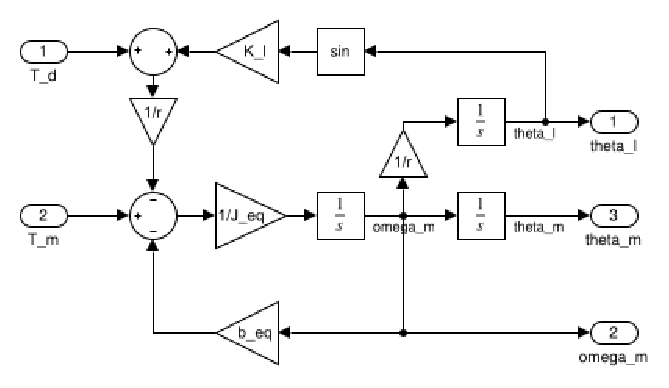
\includegraphics{2-Subsistema_Mecánico_Completo}}
    \end{adjustbox}
    \caption{Diagrama de bloques del sub-sistema mecánico completo.}
    \label{diagrama de bloques sub-sistema mecanico completo}
\end{figure}

El modelo resultante tiene un solo grado de libertad, tal como sucede con el modelo de la
carga y con el del subsistema mecánico de la máquina eléctrica sin la transmisión.
Esto se debe a la suposición de rigidez ideal y la ausencia de ``backlash'' en la reducción, 
permitiendo un ``acoplamiento directo'' de la carga al eje de la máquina eléctrica.
Dicho de otra manera, la transmisión no incorpora dinámica al subsistema mecánico.

%5.1.2
\vspace*{0.1cm}
\subsubsection{\textbf{Modelo dinámico del sistema físico completo}} este incorpora los sub-sistemas electromagnético, mecánico y térmico.

% a
\paragraph{\textbf{Modelo Global No Lineal}}
Al tratarse de un sistema no lineal de parámetros variables y con no-linealidades en las variables de estado, no se puede obtener una expresión
de la ecuación de estado y de salida del sistema en la forma:

\begin{equation*}
    \begin{cases}
        \frac{d \mathbf{x}(t)}{dt} &= A \mathbf{x}(t) + B \mathbf{u}(t)\\
        \mathbf{y}(t) &= C \mathbf{x}(t) + D \mathbf{u}(t)
    \end{cases}
\end{equation*}

Sin embargo, se puede obtener una expresión vectorial más general del modelo matemático en la forma:

\begin{equation*}
    \begin{cases}
        \frac{d \mathbf{x}(t)}{dt} &= f(\mathbf{x}(t), \mathbf{u}(t), t)\\
        \mathbf{y}(t) &= g(\mathbf{x}(t), \mathbf{u}(t), t)
    \end{cases}
\end{equation*}

Teniendo en cuenta la definición del estado del sistema (\cref{vector de estado del sistema}), la primera ecuación a considerar en la expresión vectorial de estado del sistema es la
\cref{posicion y velocidad motor}. El acoplamiento entre el sub-sistema electromagnético y el
mecánico de la máquina eléctrica se da a través del $T_m(t)$, dado por la \cref{torque electromagnetico}.
Reemplazando esta ecuación en la \cref{subsistema mecanico con parametros equivalentes} y reordenando términos,
obtenemos la segunda ecuación de estado del sistema:

\begin{equation}
    \frac{d \omega_m(t)}{dt} = \frac{3}{2} \frac{P_p i^r_{qs}(t)\left[\lambda'^r_m + (L_d - L_q) i^r_{ds}(t) \right]}{J_{eq}} - \frac{b_{eq}\omega_m(t)}{J_{eq}} - \frac{T_l(t)}{r J_{eq}}
    \label{ecuacion de estado wm}
\end{equation}

Las siguientes tres ecuaciones de estado del sistema se obtienen del balance de tensiones
en coordenadas virtuales (\cref{balance de tensiones q} \cref{balance de tensiones d}, \cref{balance de tensiones 0}).
Reemplazando en estas la relación entre $\omega_m(t)$ y $\omega_r(t)$ dada por la \cref{Relacion coordenadas electricas y mecanicas} obtenemos:
\begin{align}
    \frac{d i^r_{qs}(t)}{dt} &= -\frac{R_s(t) i^r_{qs}(t)}{L_q} - \frac{P_p \omega_m(t) \left[\lambda'^r_m + L_d i^r_{ds}(t)\right]}{L_q} + \frac{v^r_{qs}(t)}{L_q} \label{ecuacion de estado iqs}\\
    \frac{d i^r_{ds}(t)}{dt} &= -\frac{R_s(t) i^r_{ds}(t)}{L_d} + \frac{L_q P_p \omega_m(t)i^r_{qs}(t)}{L_d}  + \frac{v^r_{ds}(t)}{L_d} \label{ecuacion de estado ids}\\ 
    \frac{d i_{0s}(t)}{dt}   &= -\frac{R_s(t) i_{0s}(t)}{L_{ls}} + \frac{v_{0s}(t)}{L_{ls}}\label{ecuacion de estado i0s}
\end{align}

La última ecuación de estado se obtiene relacionando las \cref{potencia de perdidas} y \cref{balance termico estator} obteniéndose:
\begin{equation}
    \frac{d T^\circ_s(t)}{dt} = \frac{3}{2} \frac{R_s(t) \left[ i_{qs}^2(t) + i_{ds}^2(t) + 2 i_{0s}^2(t) \right]}{C_{ts}} - \frac{\left[T_s^{\circ}(t) - T_{amb}^{\circ}(t)\right]}{R_{ts}C_{ts}} 
    \label{ecuacion de estado Ts}
\end{equation}

Con objeto de abreviar la expresión de estas ecuaciones, en lugar de reemplazar el modelo completo de variación de $R_s(t)$ (\cref{Rs}) en las mismas, 
solo se deja indicada la dependencia explícita de $R_s(t)$ con respecto a $t$. Con el mismo objeto, se abreavia $R_{ts-amb}$ a $R_{ts}$.

% Ecuación vectorial de estado del sistema
\textbf{Ecuación vectorial de estado del sistema}: se obtiene expresando en forma vectorial las ecuaciones obtenidas, indicándose en la \cref{ecuacion vectorial de estado del sistema no matricial}
en forma de sistemas de ecuaciones y en forma matricial en la \cref{ecuacion vectorial de estado del sistema}

\begin{equation}
    \begin{cases} 
        \frac{d \theta_m(t)}{dt}  &= \omega_m(t)\\ 
        \frac{d \omega_m(t)}{dt}  &= \frac{1}{J_{eq}}\left(\frac{3}{2} P_p i^r_{qs}(t)\left[\lambda'^r_m + (L_d - L_q) i^r_{ds}(t) \right] - b_{eq}\omega_m(t) - \frac{1}{r}T_l(t)\right)\\ 
        \frac{d i^r_{qs}(t)}{dt}  &= \frac{1}{L_{q}}\left(-R_s(t) i^r_{qs}(t)- P_p \omega_m(t) \left[\lambda'^r_m + L_d i^r_{ds}(t)\right] + v^r_{qs}(t)\right)\\ 
        \frac{d i^r_{ds}(t)}{dt}  &= \frac{1}{L_{d}}\left(-R_s(t) i^r_{ds}(t) + P_p \omega_m(t) L_q i^r_{qs}(t)  + v^r_{ds}(t)\right)\\ 
        \frac{d i_{0s}(t)}{dt}    &= \frac{1}{L_{ls}}\left(-R_s(t) i_{0s}(t) + v_{0s}(t)\right) \\ 
        \frac{d T^\circ_s(t)}{dt} &= \frac{1}{C_{ts}}\left(\frac{3}{2} R_s(t) \left[ {i^r_{qs}(t)}^2 + {i^r_{ds}(t)}^2 + 2 {i_{0s}(t)}^2 \right] + \frac{1}{R_{ts}}\left(T^{\circ}_{amb}(t) - T_s^{\circ}(t)\right)\right)
    \end{cases}
    \label{ecuacion vectorial de estado del sistema no matricial}
\end{equation}

\begin{equation}
    \begin{bmatrix} 
        \frac{d \theta_m(t)}{dt} \\ 
        \frac{d \omega_m(t)}{dt} \\ 
        \frac{d i^r_{qs}(t)}{dt} \\ 
        \frac{d i^r_{ds}(t)}{dt} \\ 
        \frac{d i_{0s}(t)}{dt} \\ 
        \frac{d T^\circ_s(t)}{dt} 
    \end{bmatrix} 
        = 
    \begin{bmatrix} 
        \omega_m(t) \\ 
        \frac{\frac{3}{2} P_p i^r_{qs}(t)\left[\lambda'^r_m + (L_d - L_q) i^r_{ds}(t) \right]}{J_{eq}} - \frac{b_{eq}\omega_m(t)}{J_{eq}}\\ 
        -\frac{R_s(t) i^r_{qs}(t)}{L_q} - \frac{P_p \omega_m(t) \left[\lambda'^r_m + L_d i^r_{ds}(t)\right]}{L_q}\\ 
        -\frac{R_s(t) i^r_{ds}(t)}{L_d} + \frac{P_p \omega_m(t) L_q i^r_{qs}(t)}{L_d}  \\ 
        -\frac{R_s(t) i_{0s}(t) }{L_{ls}} \\ 
        \frac{\frac{3}{2} R_s(t) \left[ {i^r_{qs}(t)}^2 + {i^r_{ds}(t)}^2 + 2 {i_{0s}(t)}^2 \right]}{C_{ts}} - \frac{T_s^{\circ}(t)}{R_{ts}C_{ts}}
    \end{bmatrix}
        + 
    \begin{bmatrix} 
        0 & 0 & 0 \\ 
        0 & 0 & 0 \\ 
        \frac{1}{L_q} & 0 & 0 \\ 
        0 & \frac{1}{L_d} & 0  \\ 
        0 & 0 & \frac{1}{L_{ls}}  \\ 
        0 & 0 & 0
    \end{bmatrix} 
    \begin{bmatrix} 
        v^r_{qs}(t) \\ 
        v^r_{ds}(t) \\ 
        v_{0s}(t)
    \end{bmatrix}
        + 
    \begin{bmatrix} 
        & 0 & 0 \\
        & \frac{-1}{r J_{eq}} & 0 \\
        & 0 & 0 \\
        & 0 & 0 \\
        & 0 & 0 \\
        & 0 & \frac{1}{C_{ts} R_{ts}}
    \end{bmatrix}
    \begin{bmatrix} 
        T_l(t) \\ 
        T^{\circ}_{amb}(t) 
    \end{bmatrix}
    \label{ecuacion vectorial de estado del sistema}
\end{equation}

Con condiciones iniciales:
\begin{equation}
    \mathbf{x}(t_0) = \mathbf{x_0}
    =
    \begin{bmatrix} 
        \theta_{m0} \\ 
        \omega_{m0} \\ 
        i^r_{qs0} \\ 
        i^r_{ds0} \\ 
        i_{0s0} \\ 
        T^\circ_{s0} 
    \end{bmatrix}
\end{equation}

En la \cref{ecuacion vectorial de estado del sistema} se han separado
las relaciones que involucran a las variables de estado del sistema de las que involucran a las 
entradas de manipulación y de las que involucran a las entradas perturbación (ver \cref{vector de estado del sistema}, \cref{vector de entradas de control} y \cref{vector de entradas de perturbacion}). Se puede notar
que, aunque el sistema es no lineal en las variables de estado (no se puede obtener una expresión de la forma $Ax(t)$ para las relaciones que involucran a las variables de estado), 
sí es lineal en las entradas tanto de perturbación como de control (las relaciones que involucran a las entradas se presentan en la forma $Bu(t)$), salvo por la dependencia de $T_l(t)$ con respecto a $\theta_l(t)$ y por lo tanto con $\theta_m(t)$ 
dada por la \cref{torque de carga}.

% Ecuación vectorial de salida del sistema
\textbf{Ecuación vectorial de salida del sistema:} se obtiene considerando que la salida de interés del sistema físico es $\theta_m(t)$:
\begin{equation}
    y(t) = 
    \begin{bmatrix}
        1 & 0 & 0 & 0 & 0 & 0
    \end{bmatrix}
    \begin{bmatrix} \theta_m(t) \\ \omega_m(t) \\ i^r_{qs}(t) \\ i^r_{ds}(t) \\ i_{0s}(t) \\ T^\circ_s(t) \end{bmatrix}
    \label{ecuacion vectorial de salida del sistema}
\end{equation}

%  Diagrama de bloques del sistema físico completo
\textbf{Diagramas de bloques del sistema físico completo: } En la \cref{diagrama de bloques del sistema fisico} se muestra
el diagrama de bloques del sistema físico completo constituido por los sub-sistemas mecánico, térmico y electromagnético, cuyos diagramas
respectivos se muestran en las \cref{diagrama de bloques sub-sistema mecanico completo}, \cref{subsistema termico},
y \cref{sub-sistema electromagnetico}. A su vez, los componentes del sub-sistema electromagnético se detallan
en las \cref{diagrama de bloques I_qs}, \cref{diagrama de bloques I_ds}, \cref{diagrama de bloques I_0s}, para las corrientes ($i^r_{qs}(t)$, $i^r_{ds}(t)$, $i_{0s}(t)$ respectivamente) y en la \cref{diagrama de bloques T_m} para $T_m(t)$.
Finalmente, en las \cref{transformacion de Park} y \cref{transformacion de Park inversa} se detallan las transformaciones de Park directa e inversa respectivamente.

% Diagramas
\begin{figure}[H]
    \centering
    \begin{adjustbox}{max width=\columnwidth}
        \framebox{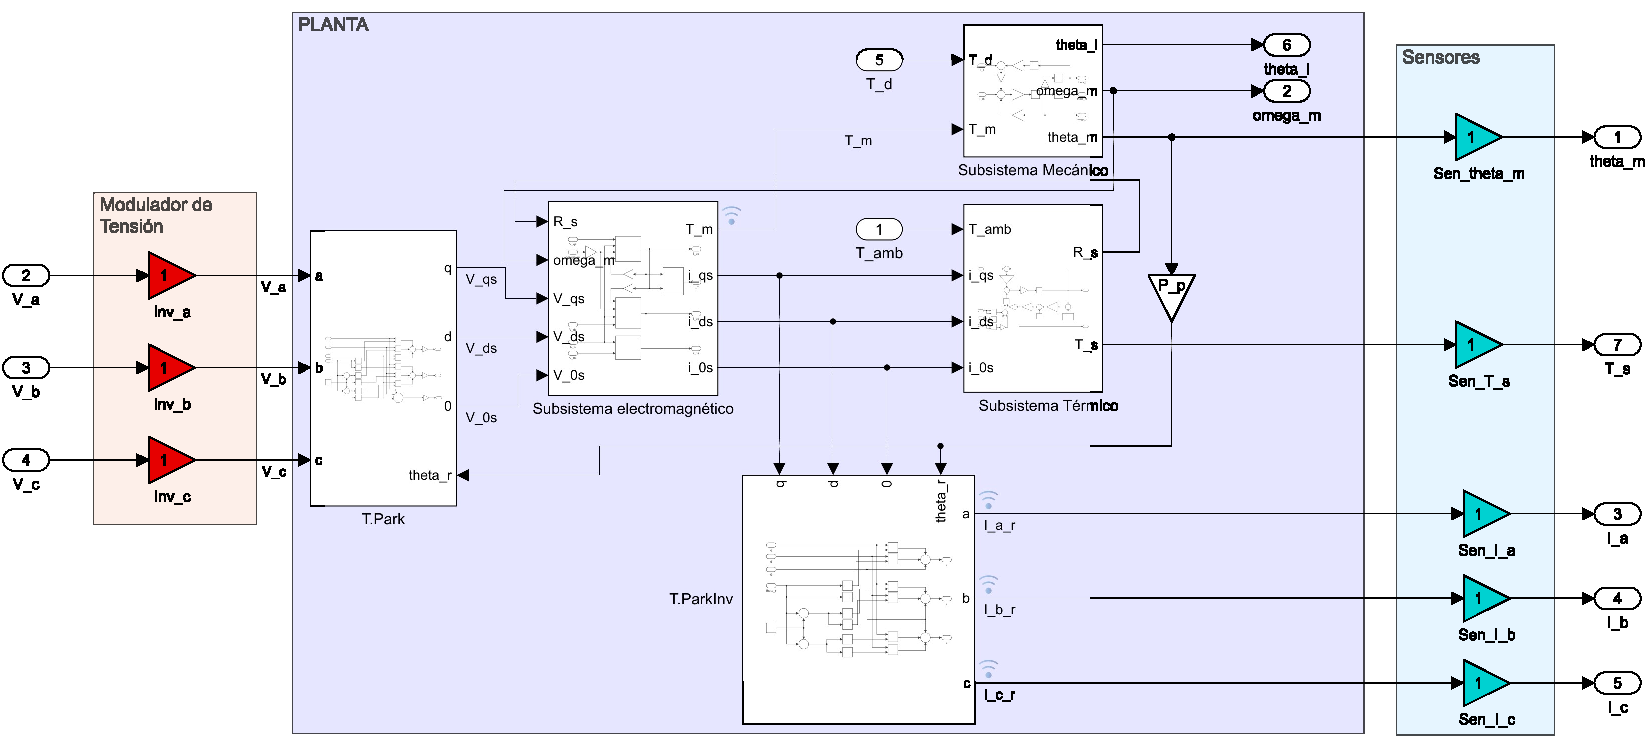
\includegraphics{3-Planta_completa}}
    \end{adjustbox}
    \caption{Diagrama de bloques completo de la planta.}
    \label{diagrama de bloques del sistema fisico}
\end{figure}

\begin{figure}[H]
    \centering
    \begin{adjustbox}{scale=0.7,max width=\columnwidth}
        \framebox{\includegraphics{4-Subsistema_Térmico}}
    \end{adjustbox}
    \caption{Diagrama de bloques del sub-sistema térmico.}
    \label{subsistema termico}
\end{figure}

\begin{figure}[H]
    \centering
    \begin{adjustbox}{scale=0.7,max width=\columnwidth}
        \framebox{\includegraphics{5-Subsistema_Electromagnético}}
    \end{adjustbox}
    \caption{Diagrama de bloques del sub-sistema electromagnético.}
    \label{sub-sistema electromagnetico}
\end{figure}

\begin{figure}[H]
    \centering
    \begin{adjustbox}{scale=0.7,max width=\columnwidth}
        \framebox{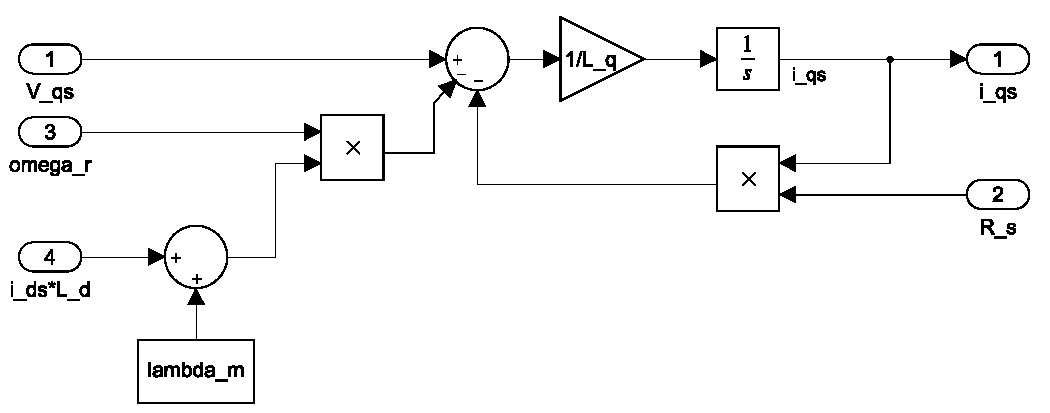
\includegraphics{6-I_qs.pdf}}
    \end{adjustbox}
    \caption{Diagrama de bloques $i^r_{qs}(t)$.}
    \label{diagrama de bloques I_qs}
\end{figure}

\begin{figure}[H]
    \centering
    \begin{adjustbox}{max width=\columnwidth}
        \framebox{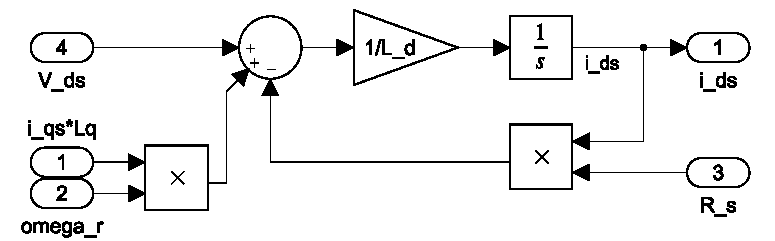
\includegraphics{7-I_ds.pdf}}
    \end{adjustbox}
    \caption{Diagrama de bloques $i^r_{ds}(t)$.}
    \label{diagrama de bloques I_ds}
\end{figure}

\begin{figure}[H]
    \centering
    \begin{adjustbox}{max width=\columnwidth}
        \framebox{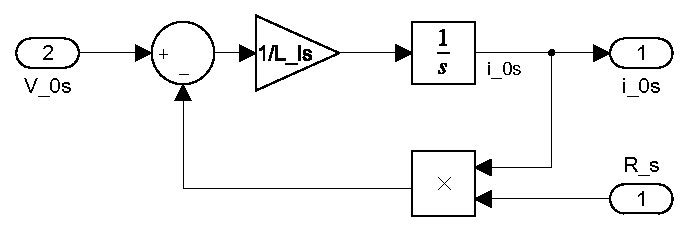
\includegraphics{8-I_0s.pdf}}
    \end{adjustbox}
    \caption{Diagrama de bloques $i_{0s}(t)$.}
    \label{diagrama de bloques I_0s}
\end{figure}

\begin{figure}[H]
    \centering
    \begin{adjustbox}{max width=\columnwidth}
        \framebox{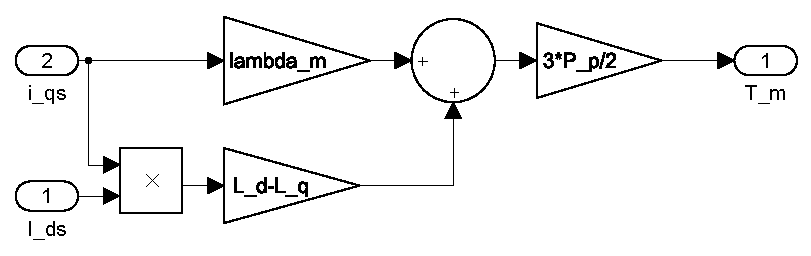
\includegraphics{9-T_m.pdf}}
    \end{adjustbox}
    \caption{Diagrama de bloques $T_m(t)$.}
    \label{diagrama de bloques T_m}
\end{figure}

\begin{figure}[H]
    \centering
    \begin{adjustbox}{max width=\columnwidth}
        \framebox{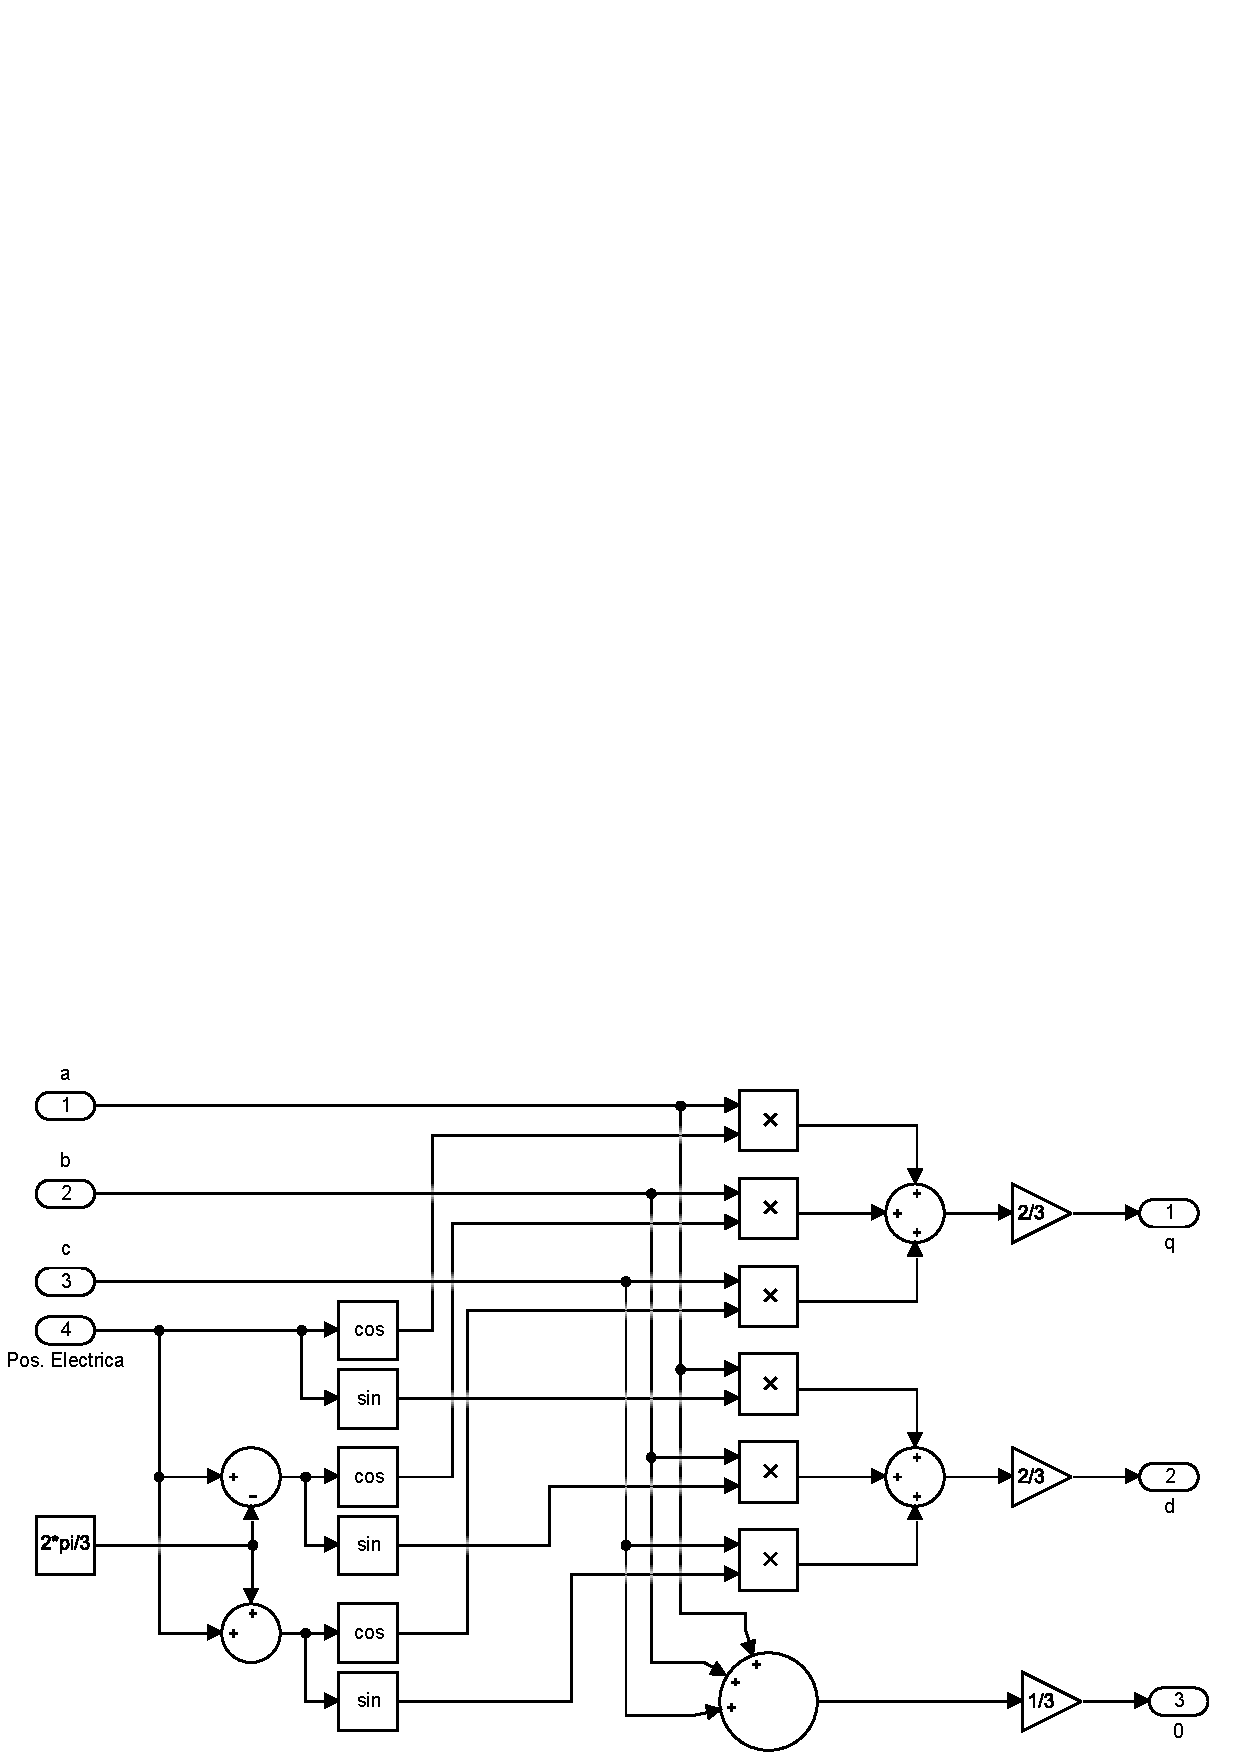
\includegraphics{10-Transformación_de_Park.pdf}}
    \end{adjustbox}
    \caption{Transformación de Park Directa.}
    \label{transformacion de Park}
\end{figure}

\begin{figure}[H]
    \centering
    \begin{adjustbox}{max width=\columnwidth}
        \framebox{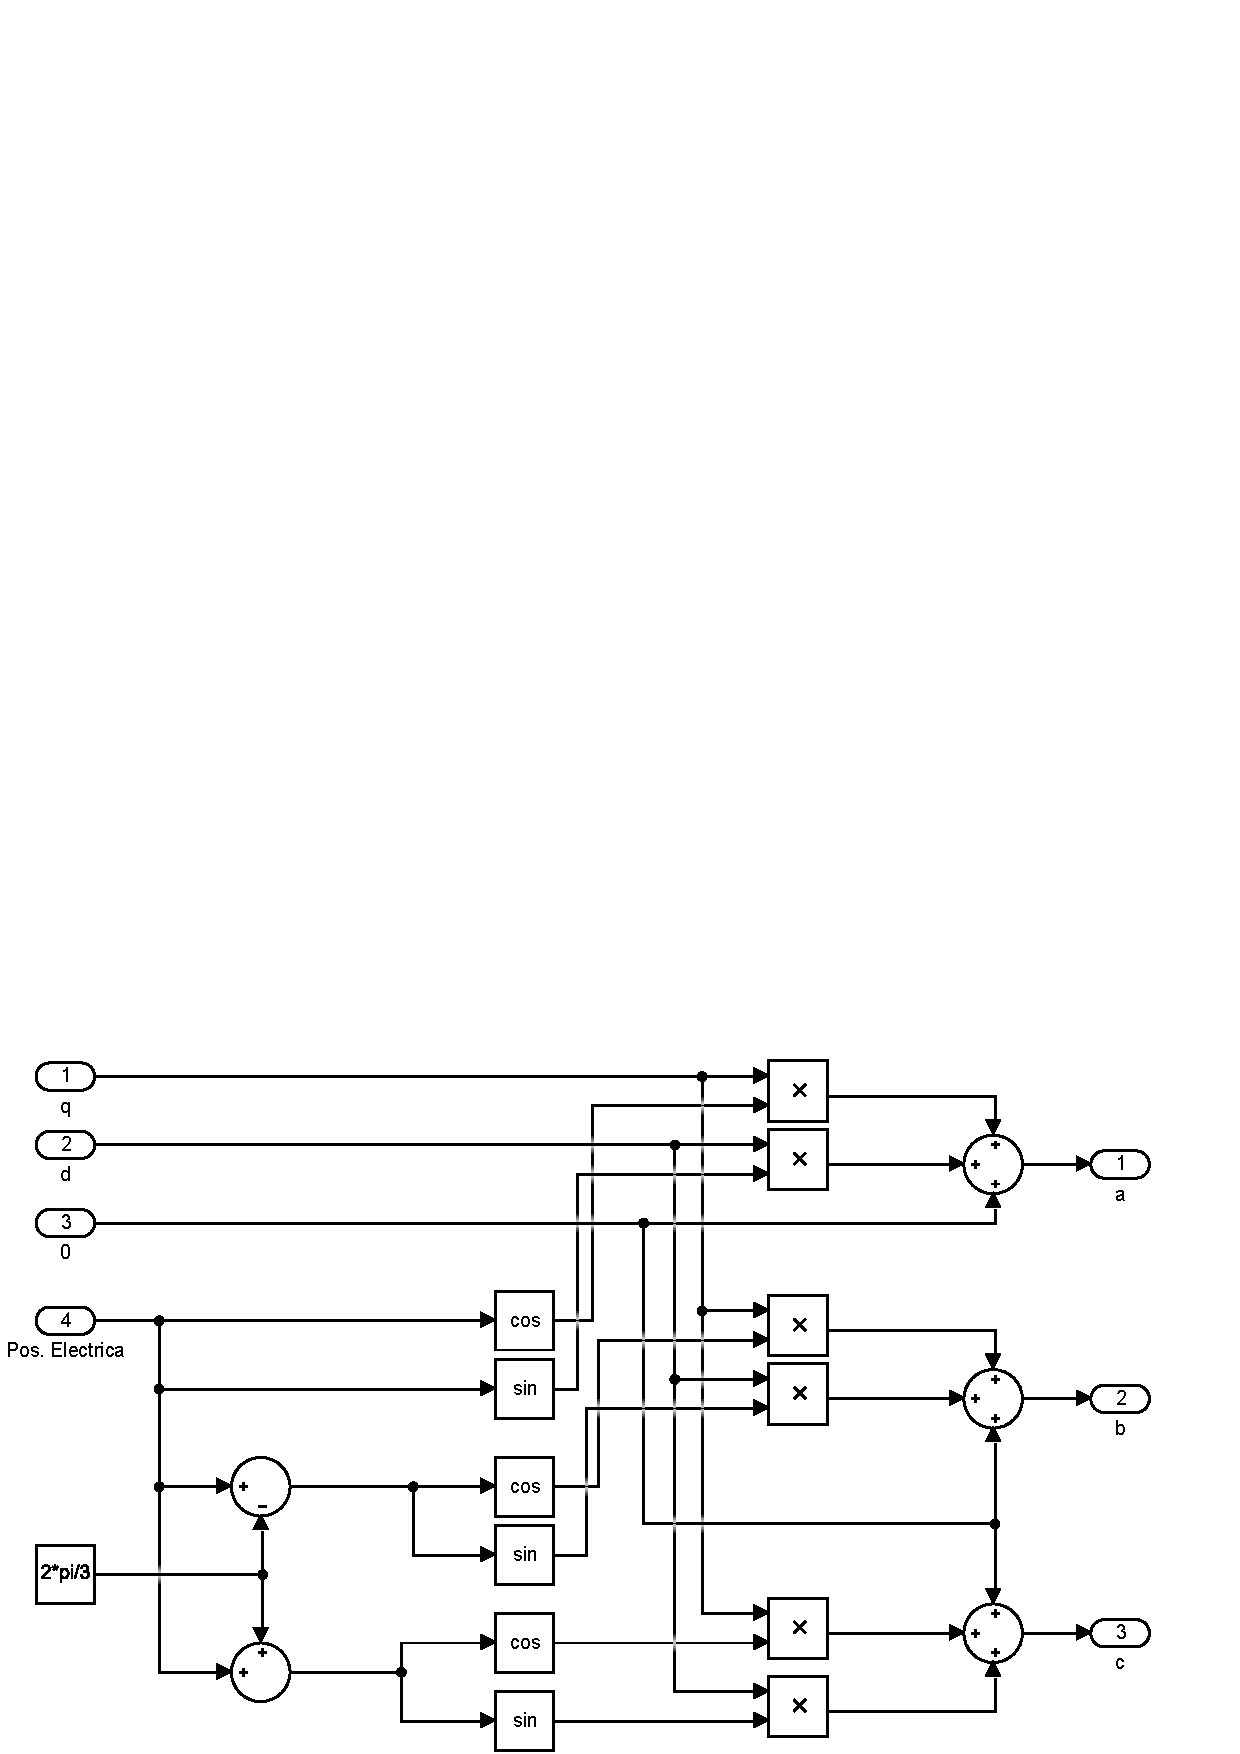
\includegraphics{11-Transformación_de_Park_Inversa.pdf}}
    \end{adjustbox}
    \caption{Transformación de Park inversa.}
    \label{transformacion de Park inversa}
\end{figure}

% 5.1.1.B Linealización Jacobiana.
\paragraph{\textbf{Linealización Jacobiana}}
Se aclara aquí que, solamente para este ejercicio, se considera un vector de entradas de perturbación modificado
con respecto al indicado en la \cref{vector de entradas} al considerar $T_l(t)$ desarrollado como se indica en la \cref{torque de carga}.
Lo que se hace es reemplazar $T_l(t)$ por $T_d(t)$ en el vector de entradas de la \cref{vector de entradas de perturbacion} lo
que cambia finalmente la definición de $\mathbf{u}(t)$. Luego, el vector
de entradas de perturbación y el vector de entradas total del sistema, para este ejercicio, son los que se indican a continuación:

\begin{equation}
    \mathbf{u_{d}}(t) = \begin{bmatrix} T_d(t) \\ T_{amb}^{\circ}(t)\end{bmatrix}\, \, \, 
    \mathbf{u}(t) = \begin{bmatrix} v^r_{qs}(t) \\ v^r_{ds}(t) \\ v^r_{0s}(t) \\ T_d(t) \\ T_{amb}^{\circ}(t) \end{bmatrix}
    \label{vector de entradas jacobi linealizado}
\end{equation}

Con esta definición del vector de entradas, la ecuación vectorial de estado del sistema es redefinida.
Por un lado se debe operar para obtener una expresión de $T_l(t)$ en función de $\theta_m(t)$ y no en función de 
$\theta_l(t)$ para luego reemplazar esta expresión en la \cref{ecuacion vectorial de estado del sistema}.
Este procedimiento se indica en la \cref{reemplazo de T_l}. Finalmente, la ecuación vectorial de estado del sistema queda expresada
como se indica en la \cref{ecuacion vectorial de estado jacobi}.

\begin{equation}
    \begin{aligned}
        \cref{relacion de velocidad en caja} \,\text{y}\, \cref{velocidad y posición de la carga}\,&\rightarrow\,\theta_l(t) = \frac{1}{r} \int_{0}^{t} \omega_m(\zeta) \, d\zeta + \theta_l(0)\\
        \cref{posicion y velocidad motor}\,&\rightarrow\,  \int_{0}^{t} \omega_m(\zeta) \, d\zeta = \theta_m(t) - \theta_m(0)\\
        \text{Reemplazando la segunda en la primera}\,&\rightarrow\,\theta_l(t) = \frac{\theta_m(t) - \theta_m(0)}{r} + \theta_l(0)\\
        \text{Consideramos que se cumple}\,&\rightarrow\,\frac{\theta_m(0)}{r} = \theta_l(0)\\
        \text{Luego}\,&\rightarrow\,\theta_l(t) = \theta_m(t)/r\\
        \text{Finalmente}\,&\rightarrow\,T_l(t) = k_l\sin\left(\frac{\theta_m(t)}{r}\right) + T_d(t)
    \end{aligned}
    \label{reemplazo de T_l}
\end{equation}

\begin{equation}
    \begin{bmatrix} 
        \frac{d \theta_m(t)}{dt} \\ 
        \frac{d \omega_m(t)}{dt} \\ 
        \frac{d i^r_{qs}(t)}{dt} \\ 
        \frac{d i^r_{ds}(t)}{dt} \\ 
        \frac{d i_{0s}(t)}{dt} \\ 
        \frac{d T^\circ_s(t)}{dt} 
    \end{bmatrix} 
        = 
    \begin{bmatrix} 
        \omega_m(t) \\ 
        \frac{\frac{3}{2} P_p i^r_{qs}(t)\left[\lambda'^r_m + (L_d - L_q) i^r_{ds}(t) \right]}{J_{eq}} - \frac{b_{eq}\omega_m(t)}{J_{eq}} - \frac{k_l\sin\left(\frac{\theta_m(t)}{r}\right)}{rJ_{eq}}\\ 
        -\frac{R_s(t) i^r_{qs}(t)}{L_q} - \frac{P_p \omega_m(t) \left[\lambda'^r_m + L_d i^r_{ds}(t)\right]}{L_q}\\ 
        -\frac{R_s(t) i^r_{ds}(t)}{L_d} + \frac{P_p \omega_m(t) L_q  i^r_{qs}(t)}{L_d}  \\ 
        -\frac{R_s(t) i_{0s}(t) }{L_{ls}} \\ 
        \frac{\frac{3}{2} R_s(t) \left[ {i^r_{qs}(t)}^2 + {i^r_{ds}(t)}^2 + 2 {i_{0s}(t)}^2 \right]}{C_{ts}} - \frac{T_s^{\circ}(t)}{R_{ts}C_{ts}}
    \end{bmatrix}
        + 
    \begin{bmatrix} 
        0 & 0 & 0 & 0 & 0 \\ 
        0 & 0 & 0 & \frac{-1}{r J_{eq}} & 0 \\ 
        \frac{1}{L_q} & 0 & 0 & 0 & 0\\ 
        0 & \frac{1}{L_d} & 0 & 0 & 0 \\ 
        0 & 0 & \frac{1}{L_{ls}}  & 0 & 0 \\ 
        0 & 0 & 0 & 0 & \frac{1}{C_{ts} R_{ts}}
    \end{bmatrix} 
    \begin{bmatrix} 
        v^r_{qs}(t) \\ 
        v^r_{ds}(t) \\ 
        v_{0s}(t) \\
        T_d(t) \\ 
        T^{\circ}_{amb}(t)
    \end{bmatrix}
    \label{ecuacion vectorial de estado jacobi}
\end{equation}

En el modelo de pequeñas desviaciones locales $\delta \mathbf{x}(t)$ respecto de los puntos de operación $\mathbf{X}_o(t)$
se hacen las siguientes consideraciones.

\begin{equation}
    \begin{cases}
    \mathbf{x}(t)  &= \mathbf{X}_o(t) + \mathbf{\delta x}(t)\\
    \mathbf{\delta x}(0) &\equiv \mathbf{0}
    \end{cases}
    \label{pequeñas desviaciones}
\end{equation}

La ecuación del \textbf{espacio de operación global NL cuasi-estacionario} es:

\begin{equation}
    \begin{cases}
    \frac{d\mathbf{X}_o(t)}{dt} =  \mathbf{f}(\mathbf{X}_o(t), \mathbf{U}_o(t)) \approx 0/\text{const};  \mathbf{X}_o(0) \equiv \mathbf{x}_0\\
    \mathbf{Y}_o(t) = C \mathbf{X}_o(t)
    \end{cases}
    \label{modelo de operacion NL cuasi-estacionario}
\end{equation}

Para nuestro sistema esto queda expresado como se indica en la \cref{modelo de operacion NL cuasi_estacionario desarrollado} para la ecuación de estado, y en la \cref{condiciones inciales cuasi-estacionario} para las condiciones iniciales.
En las mismas, el sub-indice $-o$ indica los valores de las variables en el punto de operación.

\begin{equation}
    \begin{bmatrix}
        \frac{d \theta_{m-o}(t)}{dt}\\
        \frac{d \omega_{m-o}(t)}{dt}\\
        \frac{d i^r_{qs-o}(t)}{dt}\\
        \frac{d i^r_{ds-o}(t)}{dt}\\
        \frac{d i_{0s-o}(t)}{dt}\\
        \frac{d T^\circ_{s-o}(t)}{dt}
    \end{bmatrix}
    =
    \begin{cases}
        \omega_{m-o}(t) &\approx \omega_{m0}\\
        \frac{1}{J_{eq}}\left[\frac{3}{2} P_p i^r_{qs-o}(t)\left[\lambda'^r_m + (L_d - L_q) i^r_{ds-o}(t) \right] - b_{eq}\omega_{m-o}(t) - \frac{k_l}{r}\sin\left(\frac{\theta_{m-o}(t)}{r}\right) - \frac{1}{r}T_{d-o}(t)\right] &\approx 0\\
        \frac{1}{L_q}\left[-R_{s-o}(t) i^r_{qs-o}(t)- P_p \omega_{m-o}(t) \left[\lambda'^r_m + L_d i^r_{ds-o}(t)\right] + v^r_{qs-o}(t)\right] &\approx 0\\ 
        \frac{1}{L_d}\left[-R_{s-o}(t) i^r_{ds-o}(t) + P_p \omega_{m-o}(t) L_q  i^r_{qs-o}(t) + v^r_{ds-o}(t)\right] &\approx 0\\ 
        \frac{1}{L_{ls}}\left[-R_{s-o}(t) i_{0s}(t) + v_{0s-o}(t)\right] &\approx 0\\ 
        \frac{3}{2}\frac{R_{s-o}(t)}{C_{ts}} \left[ {i^r_{qs-o}}^2(t) + {i^r_{ds-o}(t)}^2 + 2 {i_{0s-o}(t)}^2 \right] + \frac{1}{R_{ts}C_{ts}}\left[T^{\circ}_{amb-o}(t) - T_{s-o}^{\circ}(t)\right] &\approx 0
    \end{cases}
    \label{modelo de operacion NL cuasi_estacionario desarrollado}
\end{equation}


\begin{equation}
    \mathbf{X_o}(0)
    =
    \begin{bmatrix} 
        \theta_{m-o}(0) \\ 
        \omega_{m-o}(0) \\ 
        i^r_{qs-o}(0) \\ 
        i^r_{ds-o}(0)\\ 
        i_{0s-o}(0)\\ 
        T^\circ_{s-o}(0)
    \end{bmatrix}
    =
    \begin{bmatrix} 
        \theta_{m0} \\ 
        \omega_{m0} \\ 
        i^r_{qs0} \\ 
        i^r_{ds0} \\ 
        i_{0s0} \\ 
        T^\circ_{s0} 
    \end{bmatrix}
    \label{condiciones inciales cuasi-estacionario}
\end{equation}

Consideramos relevante hacer aquí un análisis al respecto
del espacio de operación global NL para este modelo del sistema físico
en particular.

Si, en lugar de la restricción débil señalada en la \cref{modelo de operacion NL cuasi-estacionario}
se toma la restricción fuerte dada por la \cref{restriccion fuerte}, y si se toman en cuenta
las condiciones iniciales del modelo señaladas en la \cref{condiciones inciales cuasi-estacionario} y 
la evolución de $\theta_m(t)$ dada por la \cref{posicion y velocidad motor}, tendremos un
punto de operación definido como en la \cref{punto de operacion}.


\begin{equation}
    \frac{d\mathbf{X}_o(t)}{dt} =  \mathbf{f}(\mathbf{X}_o(t), \mathbf{U}_o(t)) \equiv 0/\text{const}
    \label{restriccion fuerte}
\end{equation}

\begin{equation}
    \mathbf{X_o}(t)
    =
    \begin{bmatrix} 
        \theta_{m-o}(t) \\ 
        \omega_{m-o}(t) \\ 
        i^r_{qs-o}(t) \\ 
        i^r_{ds-o}(t)\\ 
        i_{0s-o}(t)\\ 
        T^\circ_{s-o}(t)
    \end{bmatrix}
    =
    \begin{bmatrix} 
        \int_{0}^{t} \omega_{m-o}(0) d\tau + \theta_{m-o}(0)\\
        \omega_{m-o}(0)\\
        i^r_{qs-o}(0) \\
        i^r_{ds-o}(0)\\
        i_{0s-o}(0)\\
        T^\circ_{s-o}(0)
    \end{bmatrix}
    =
    \begin{bmatrix} 
        \omega_{m0}t + \theta_{m0}\\
        \omega_{m0} \\ 
        i^r_{qs0} \\ 
        i^r_{ds0} \\ 
        i_{0s0} \\ 
        T^\circ_{s0} 
    \end{bmatrix}
    \label{punto de operacion}
\end{equation}

Reemplazamos lo obtenido en la \cref{punto de operacion} en la \cref{modelo de operacion NL cuasi_estacionario desarrollado}
y destacamos la ecuación de estado asociada a $\omega_m(t)$.

\begin{equation}    
    \frac{1}{J_{eq}}\left[\frac{3}{2} P_p i^r_{qs0}\left[\lambda'^r_m + (L_d - L_q) i^r_{ds0} \right] - b_{eq}\omega_{m0} - \frac{k_l}{r}\sin\left(\frac{\omega_{m0}t + \theta_{m0}}{r}\right) - \frac{1}{r}T_{d0}\right] = 0
    \label{ecuacion de estado omega_m espacio NL de operacion}
\end{equation}

Se puede ver que esta ecuación
tiene  una dependencia explícita de $t$, no solamente de las variables de 
estado y de las entradas en el punto de operación. La \cref{ecuacion de estado omega_m espacio NL de operacion}
se puede expresar de forma simplificada, para mostrar nuestro punto, como:

\begin{equation}    
    cte - \frac{k_l}{r}\sin\left(\frac{\omega_{m0}t + \theta_{m0}}{r}\right) - \frac{1}{r}T_{d-o}(t) = 0
    \label{ecuacion de estado omega_m espacio NL de operacion simplificada}
\end{equation}

Condición que se puede satisfacer solo bajo dos supuestos distintos indicados en la \cref{condiciones de satisfaccion}.
La primera de ellas implica tener control sobre la entrada de perturbación $T_{d-o}$, lo cual
no es posible por definición, o bien si se tuviera un contrapeso que equilibre el torque
gravitacional producido por el brazo y la masa que transporta en su extremo. La segunda condición
elimina la dependencia explícita de $t$ y no requiere control sobre la entrada de perturbación para
lograrse.

\begin{equation}
    \begin{cases}
        T_{d-o}(t) &= cte - \frac{k_l}{r}\sin\left(\frac{\omega_{m0}t + \theta_{m0}}{r}\right)\\
        \omega_{m0} &= 0
    \end{cases}
    \label{condiciones de satisfaccion}
\end{equation}

Cuando se asume la segunda condición de la \cref{condiciones de satisfaccion},
la \cref{modelo de operacion NL cuasi_estacionario desarrollado} queda como se indica en la 
\cref{modelo de operacion NL cuasi_estacionario desarrollado reducido}. En la que
además se toma $v_{0s-o}(t) \equiv 0$ al tratarse de un sistema de
tensiones trifásico simétrico balanceado. Eso da por resultado $i_{0s0} = 0$,
al ser $R_{s-o} \neq 0$ para las temperaturas normales de operación, y se reemplaza directamente en la 
ecuación de estado de la $T^{\circ}_{s}$.

\begin{equation}
    \begin{cases}
        \omega_{m0} &= 0\\
        \frac{1}{J_{eq}}\left[\frac{3}{2} P_p i^r_{qs0}\left[\lambda'^r_m + (L_d - L_q) i^r_{ds0} \right] - \frac{k_l}{r}\sin\left(\frac{\theta_{m0}}{r}\right) - \frac{1}{r}T_{d-o}\right] &= 0\\
        \frac{1}{L_q}\left[-R_{s-o} i^r_{qs0} + v^r_{qs-o}\right] &= 0 \Rightarrow i^r_{qs0} = v^r_{qs-o}/R_{s-o}\\ 
        \frac{1}{L_d}\left[-R_{s-o} i^r_{ds0} + v^r_{ds-o}\right] &= 0 \Rightarrow i^r_{ds0} = v^r_{ds-o}/R_{s-o}\\ 
        \frac{1}{L_{ls}}\left[-R_{s-o} i_{0s}\right] &= 0 \Rightarrow i_{0s} = 0\\ 
        \frac{3}{2}\frac{R_{s-o}}{C_{ts}} \left[ {i^r_{qs0}}^2+ {i^r_{ds0}}^2 \right] + \frac{1}{R_{ts}C_{ts}}\left[T^{\circ}_{amb-o} - T_{s0}^{\circ}\right] &= 0
    \end{cases}
    \label{modelo de operacion NL cuasi_estacionario desarrollado reducido}
\end{equation}

Considerando este último caso, es interesante presentar las curvas que permitan obtener las entradas
de control que es necesario aplicar para obtener una posición deseada
del brazo, dado un vector de entradas de perturbación constantes.

En \cref{T_m en función de la posición y T_do} representamos
el $T_{m-o}$ que se requiere para una preturbación $T_{d-o}$ dada,
en función de la posición del brazo. En donde se
consideran los valores extremos de $T_{d-o}$ y un
un valor de $k_l = 9.807 \left[N.m\right]$, ambos en los rangos
dados en \cite{c1}.

\begin{figure}[H]
    \centering
    \begin{adjustbox}{scale = 0.6}
        \framebox{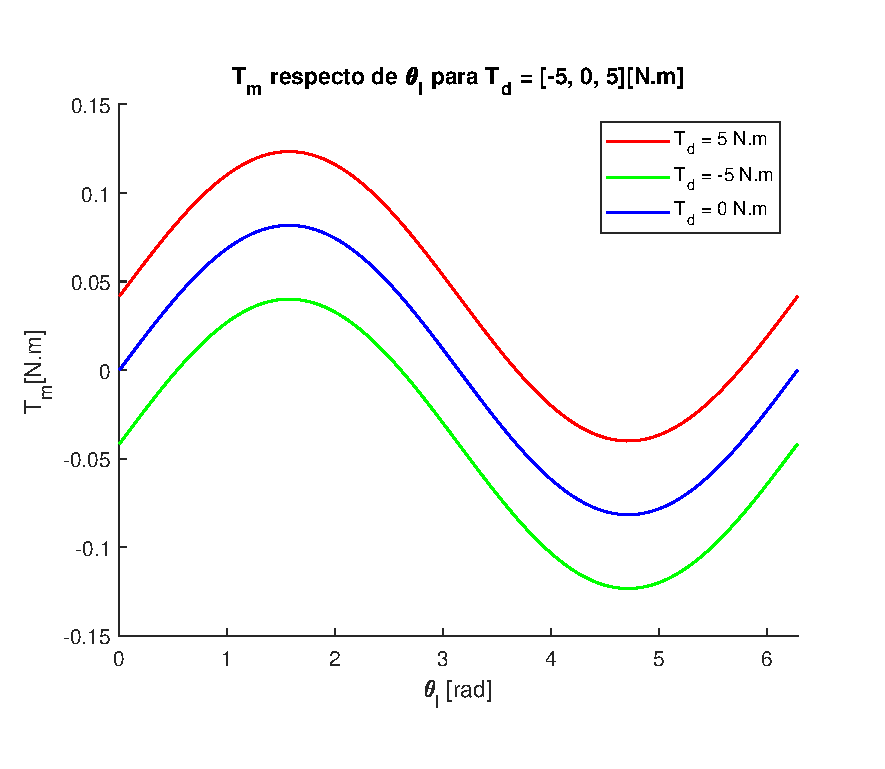
\includegraphics{12-T_m_vs_thetha_vd_Td.pdf}}
    \end{adjustbox}
    \caption{$T_m$ respecto a $T_{d-o}$ y $\theta_l$.}
    \label{T_m en función de la posición y T_do}
\end{figure}

Luego, dado un valor de corriente total $i^{r}_{qd0s-o}$ como se indica en la \cref{corriente total}, junto con un
ángulo $\beta$, que se pueden relacionar
gráficamente como se muestra en la \cref{restriccion de corriente maxima}, podemos expresar
las curvas de $T_{m-o}$ en función de $i^{r}_{qd0s-o}$ con $\beta$ como parámetro, las que
se muestran en la \cref{T_m respecto a i_qd0s-o} y que responden a la \cref{ecuación T_m respecto a i_qd0s-o}.


\begin{equation}
    \left(i^{r}_{qd0s-o}\right)^2 = \left(i^{r}_{qs0}\right)^2 + \left(i^{r}_{ds0}\right)^2
    \label{corriente total}
\end{equation}

\begin{equation}
    T_{m-o} = \frac{3}{2} P_p i^r_{qd0s-o}\sin(\beta)\left[\lambda'^r_m + (L_d - L_q) i^r_{qd0s-o}\cos(\beta)\right]
    \label{ecuación T_m respecto a i_qd0s-o}
\end{equation}

\begin{figure}[H]
    \centering
    \begin{adjustbox}{scale = 0.6}
        \framebox{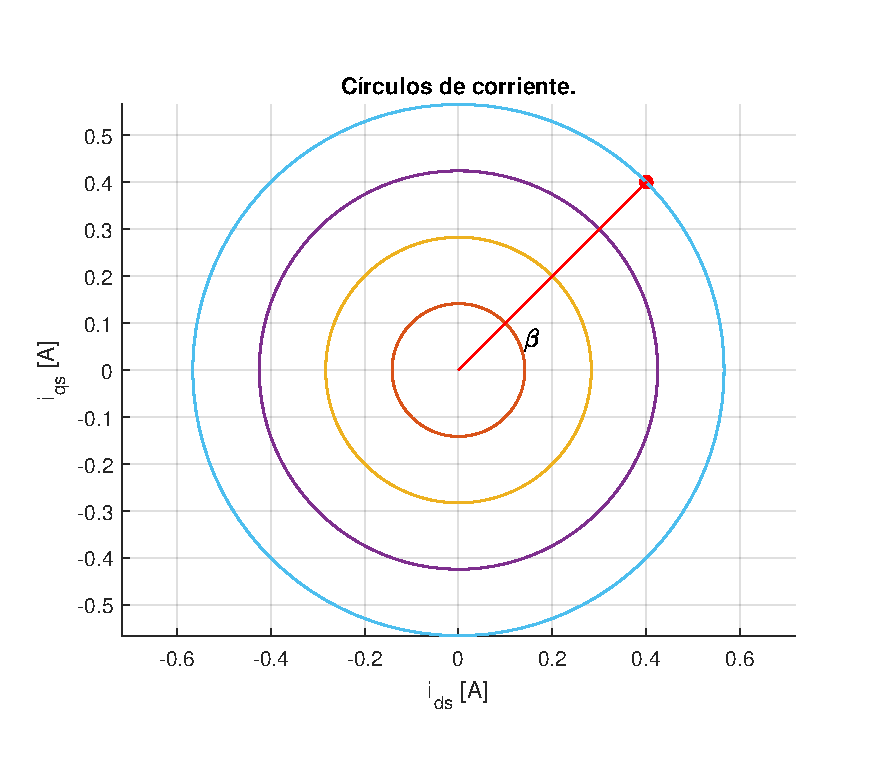
\includegraphics{13-Circulos_de_corriente.pdf}}
    \end{adjustbox}
    \caption{Circulos de corriente total en coordenadas virtuales.}
    \label{restriccion de corriente maxima}
\end{figure}

\begin{figure}[H]
    \centering
    \begin{adjustbox}{scale = 0.6}
        \framebox{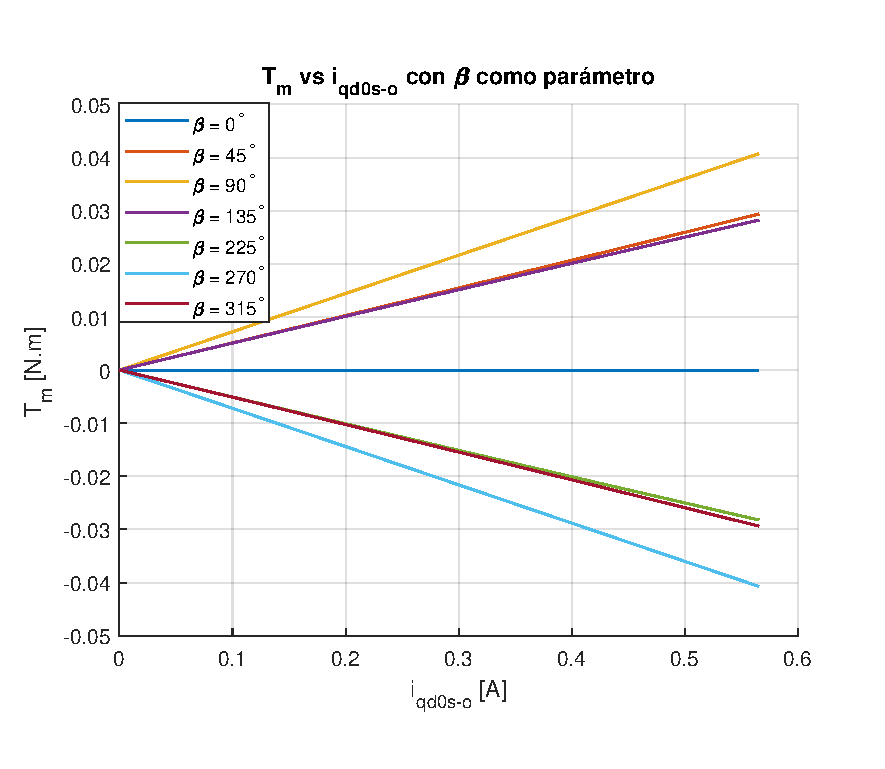
\includegraphics{14-T_m_vs_corriente_vs_beta.pdf}}
    \end{adjustbox}
    \caption{$T_m$ respecto de $i^r_{qd0s-o}$ con parámetro $\beta$.}
    \label{T_m respecto a i_qd0s-o}
\end{figure}

De la \cref{modelo de operacion NL cuasi_estacionario desarrollado reducido}
se puede obtener $T^{\circ}_{s-o}$ a partir del conocimiento de la corriente total. Esto se expresa en la
\cref{T_s respecto a la corriente total} y da como resultado la gráfica mostrada en la \cref{grafica T_s respecto a la corriente}, en donde
se grafica la $T^{\circ}_{s-o}$ respecto a $i^{r}_{qd0s-o}$ con $T^{\circ}_{amb-o}$ como parámetro.

\begin{equation}
    T^{\circ}_{s-o} = \frac{\frac{3}{2}R_{sREF}\left(\alpha_{cu}T^{\circ}_{sREF} - 1\right)\left(i^{r}_{qd0s-o}\right)^2 - \frac{T^{\circ}_{amb-o}}{R_{ts-amb}}}{\frac{3}{2}R_{sREF}\alpha_{cu}\left(i^{r}_{qd0s-o}\right)^2 - \frac{1}{R_{ts-amb}}}
    \label{T_s respecto a la corriente total}
\end{equation}

\begin{figure}[H]
    \centering
    \begin{adjustbox}{scale = 0.6}
        \framebox{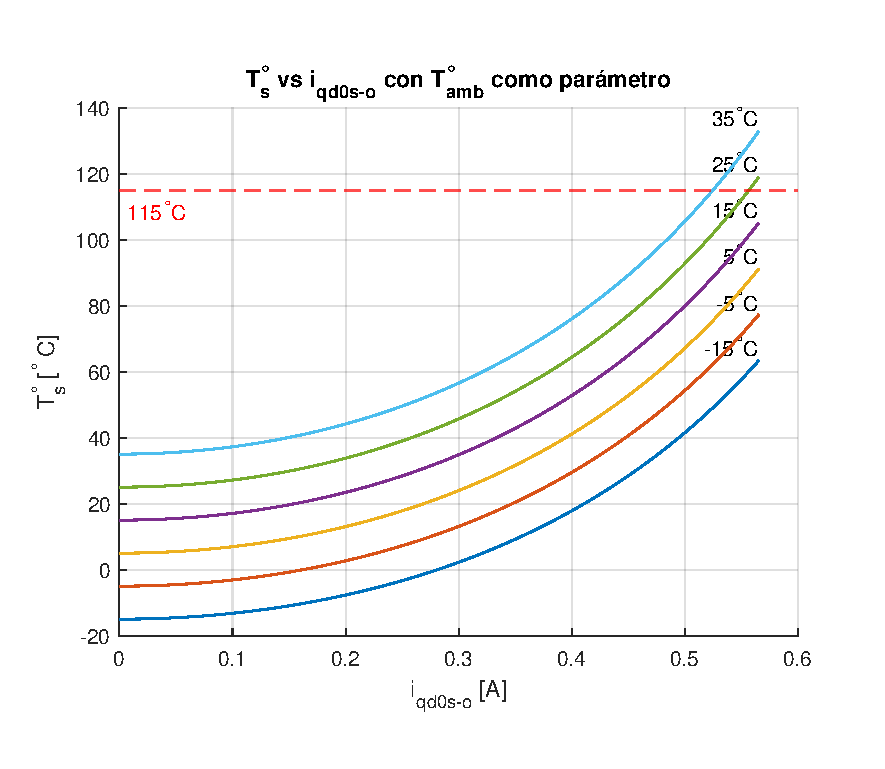
\includegraphics{15-Temperatura_vs_corriente.pdf}}
    \end{adjustbox}
    \caption{$T^{\circ}_{s-o}$ respecto de $i^r_{qd0s-o}$ con parámetro $T^{\circ}_{amb}$.}
    \label{grafica T_s respecto a la corriente}
\end{figure}

Por otro lado, el \textbf{Modelo dinámico LPV} se indica en la \cref{modelo de pequeñas desviaciones}:

\begin{equation}
    \begin{cases}
        \frac{d}{dt} \mathbf{\delta x}(t) &\approx A(t) \mathbf{\delta x}(t) + B(t) \mathbf{\delta u}(t); \mathbf{\delta x}(0) \equiv \mathbf{0}\\
        \mathbf{\delta y}(t) &= C\mathbf{\delta x}(t)
    \end{cases}
    \label{modelo de pequeñas desviaciones}
\end{equation}

En donde las matrices $A(t)$ y $B(t)$  vienen dadas por la siguiente:

\begin{equation}
    A(t) = \left[ \left. \frac{\mathbf{\partial f}}{\mathbf{\partial x}} \right|_{o}(t) \right] =
    \begin{bmatrix}
        \left.\frac{\partial}{\partial x}\left( \frac{d \theta_m(t)}{dt}\right)\right|_{o} \\ 
        \left.\frac{\partial}{\partial x}\left( \frac{d \omega_m(t)}{dt}\right)\right|_{o} \\
        \left.\frac{\partial}{\partial x}\left( \frac{d i^r_{qs}(t)}{dt}\right)\right|_{o} \\ 
        \left.\frac{\partial}{\partial x}\left( \frac{d i^r_{ds}(t)}{dt}\right)\right|_{o} \\ 
        \left.\frac{\partial}{\partial x}\left( \frac{d i^r_{0s}(t)}{dt}\right)\right|_{o} \\ 
        \left.\frac{\partial}{\partial x}\left( \frac{d T^\circ_s(t)}{dt}\right)\right|_{o} 
    \end{bmatrix}\quad
    B(t) = \left[ \left. \frac{\mathbf{\partial f}}{\mathbf{\partial u}} \right|_{o}(t) \right] =
    \begin{bmatrix}
        0 & 0 & 0 & 0 & 0\\
        0 & 0 & 0 & \frac{-1}{r J_{eq}} & 0\\
        \frac{1}{L_q} & 0 & 0 & 0 & 0\\
        0 & \frac{1}{L_d} & 0 & 0 & 0\\
        0 & 0 & \frac{1}{L_d} & 0 & 0\\
        0 & 0 & 0 & 0 & \frac{1}{C_{ts} R_{ts}}
    \end{bmatrix}
    \label{matriz_AB}
\end{equation}

Las derivadas parciales indicadas para $A(t)$ en la \cref{matriz_AB} son:

\begin{equation}
    \begin{aligned}
        \left.\frac{\partial}{\partial x}\left( \frac{d \theta_m(t)}{dt}\right) \right|_{o} &= \begin{bmatrix} 0 & 1 & 0 & 0 & 0 & 0 \end{bmatrix}\\
        \left.\frac{\partial}{\partial x}\left( \frac{d \omega_m(t)}{dt}\right) \right|_{o}&= \begin{bmatrix}
        \frac{-K_{l} \cos\left(\frac{\theta_{m-o}}{r}\right)}{J_{eq} r^2}& \frac{-b_{eq}}{J_{eq}} & \frac{3 P_p \left(\lambda'^r_m + i^r_{ds-o} \left(L_d-L_q\right)\right)}{2 J_{eq}} & \frac{3 P_p i^r_{qs-o} \left(L_d-L_q\right)}{2 J_{eq}} & 0 & 0 
        \end{bmatrix}\\
        \left.\frac{\partial}{\partial x}\left( \frac{d i^r_{qs}(t)}{dt}\right) \right|_{o}&= \begin{bmatrix} 
        0 & \frac{-P_p \left(i^r_{ds-o} L_d+\lambda'^r_m\right)}{L_q} & \frac{-R_{s-o}}{L_q} & \frac{-L_d P_p \omega_{m-o}}{L_q} & 0 & \frac{-R_{sREF} \alpha_{cu} i^r_{qs-o}}{L_q} 
        \end{bmatrix}\\
        \left.\frac{\partial}{\partial x}\left( \frac{d i^r_{ds}(t)}{dt}\right) \right|_{o}&= \begin{bmatrix} 
        0 & \frac{L_q P_p i^r_{qs-o}}{L_d} & \frac{L_q P_p \omega_{m-o}}{L_d} & \frac{-R_{s-o}}{L_d} & 0 & \frac{-R_{sREF} \alpha_{cu} i^r_{ds-o}}{L_d} 
        \end{bmatrix}\\
        \left.\frac{\partial}{\partial x}\left( \frac{d i_{0s}(t)}{dt}\right) \right|_{o}&= \begin{bmatrix} 
        0 & 0 & 0 & 0 & \frac{-R_{s-o}}{L_{ls}} & \frac{-R_{sREF} \alpha_{cu} i_{0s-o}}{L_{ls}} 
        \end{bmatrix}\\
        \left.\frac{\partial}{\partial x}\left( \frac{d T^\circ_{s}(t)}{dt}\right)\right|_{o} &= \begin{bmatrix} 
        0 & 0 & \frac{3 R_{s-o} i^r_{qs-o}}{C_{ts}} & \frac{3 R_{s-o} i^r_{ds-o}}{C_{ts}} & \frac{6 R_{s-o} i^r_{0s-o}}{C_{ts}} & \frac{3 R_{sREF} \alpha_{cu} \left({i^r_{ds-o}}^2+2 {i^r_{0s-o}}^2+{i^r_{qs-o}}^2\right)}{2 C_{ts}} - \frac{1}{C_{ts} R_{ts}} 
        \end{bmatrix}\\
    \end{aligned}
    \label{gradientesA}
\end{equation}

Nota: Por motivos de legibilidad del modelo matemático LPV completo, decidimos conservar la expresión en esta forma desagregada.

\paragraph{\textbf{Linealización Por Realimentación No Lineal}}
Dado que la dinámica del sub-sistema térmico es
más lenta, comparativamente, que la dinámica del resto del sistema físico, lo que da por resultado
una variación relativamente lenta de la $T^{\circ}_s(t)$ y por lo tanto de la $R_s(t)$,
en este análisis no se tendrá en cuenta el acoplamiento no lineal con el sub-sistema térmico (el que se da a través de la $R_s(t)$), 
pero sí se considerará su dinámica lineal. Además, teniendo en cuenta que el sistema de tensiones $v_{abcs}(t)$ es un sistema
simétrico balanceado, podemos asumir $v_{0s}(t) \equiv 0$, lo que da por resultado $i_{0s}(t) \equiv 0$ en estado permanente. Esto sumado a la especificación $i^{r}_{ds}(t)\equiv0$, 
la que imponemos directamente, hace que se pueda considerar para el análisis, un vector de estado reducido:

\begin{equation}
    \mathbf{x}(t) = \begin{bmatrix} \theta_m(t) \\ \omega_m(t) \\ i^r_{qs}(t)\end{bmatrix}
    \label{vector de estado reducido}
\end{equation}

Las ecuaciones de estado resultantes se indican en la \cref{ecuacion con ids=0}.
En la que se puede observar que se toma $R_s$ constante en lugar  de $R_s(t)$ al
no considerar el acoplamiento con el sub-sistema térmico. En concreto
se tomará para este ejercicio y mientras no se indique otra cosa, el valor de 
$R_s(t)$ a la temperatura de referencia de $40^\circ C$ de $1.02 \, \Omega$, \cite{c1}%vendría la cita a la parte de los parámetros en la guía.

\begin{equation}
	\begin{cases}
		\frac{d \theta_m(t)}{dt}  &= {\omega}_m(t)\\
		\frac{d \omega_m(t)}{dt}  &= \frac{3}{2} \frac{P_p i^r_{qs}(t)\lambda^{'r}_m}{J_{eq}} - \frac{b_{eq}\omega_m(t)}{J_{eq}} - \frac{T_l(t)}{r J_{eq}}\\
		\frac{d i^r_{qs}(t)}{dt}  &= -\frac{R_s i^r_{qs}(t)}{L_q} - \frac{P_p \omega_m(t) \lambda'^r_m}{L_q}+ \frac{v^r_{qs}(t)}{L_q}
    \end{cases}
	\label{ecuacion con ids=0}
\end{equation}

Expresándolo en forma de espacio de estados se obtienen las
\textbf{ecuaciones matriciales LTI de estado y de salida (con estado inicial genérico)}
como se indica:

\begin{equation}
	\begin{cases}
		\begin{bmatrix}
			\frac{d \theta_m(t)}{dt} \\ 
			\frac{d \omega_m(t)}{dt}\\
			\frac{d i^r_{qs}(t)}{dt}  
		\end{bmatrix}
		 &= 
		 \begin{bmatrix}
		 	0 & 1 & 0 \\ 
		 	0 & - \frac{b_{eq}}{J_{eq}} & \frac{3}{2} \frac{P_p \lambda^{'r}_m}{J_{eq}} \\
		 	0 &  - \frac{P_p  \lambda^{'r}_m}{L_q} & -\frac{R_s}{L_q}
		 \end{bmatrix}
		 \begin{bmatrix}
		 	{\theta}_m(t) \\ 
		 	{\omega}_m(t)\\
		 	{i}^r_{qs}(t)  
		 \end{bmatrix}
		 +
		 \begin{bmatrix}
		 	0 \\ 
		 	0\\
		 	\frac{1}{L_q}  
		 \end{bmatrix}
		 v^r_{qs}(t)+
		 \begin{bmatrix}
		 	0 \\ 
		 	- \frac{1}{r J_{eq}}\\
		 	0 
		 \end{bmatrix} T_l(t)\,\,; \mathbf{x}(0) = \mathbf{x_0}\\
		 y(t) &= \begin{bmatrix}
		 		1 & 0 & 0
		 	 \end{bmatrix}
		 	 \begin{bmatrix}
		 	 	{\theta}_m(t) \\ 
		 	 	{\omega}_m(t)\\
		 	 	{i}^r_{qs}(t)
		 	 \end{bmatrix}
	\end{cases}
	\label{ecuacion matricial con ids=0}
\end{equation}

La dinámica resultante del sub-sistema térmico,
indicada en la \cref{dinamica sub-sistema térmico},
se obtiene al reemplazar en la ecuación de estado de la $T^{\circ}_s$
(\cref{ecuacion vectorial de estado del sistema}) las consideraciones indicadas al inicio de este inciso al
respecto de las corrientes. En la misma, el término $\frac{3}{2}\frac{R_{s}}{C_{ts}} {i^r_{qs}(t)}^2$ representa
la $P_{sperd}(t)$, que al considerarse como entrada junto con la $T^{\circ}_{amb}(t)$, ponen de
manifiesto la dinámica lineal indicada.

\begin{equation}
    \frac{d T^\circ_{s}(t)}{dt} = \frac{3}{2}\frac{R_{s}}{C_{ts}} {i^r_{qs}(t)}^2 + \frac{1}{R_{ts}C_{ts}}\left[T^{\circ}_{amb}(t) - T_{s}^{\circ}(t)\right]
    \label{dinamica sub-sistema térmico}
\end{equation}

El \textbf{diagrama de bloques de estado del LTI equivalente en forma desagregada}, junto con la
dinámica de la $T^{\circ}_s(t)$, se puede observar en la \cref{diagrama de bloques LTI equivalente}. Mientras
que en la \cref{diagrama de bloques LTI equivalente i0s e ids} se muestra la dinámica de la
$i^r_{ds}(t)$ y la $i_{0s}(t)$ bajo las especificaciones indicadas.

\begin{figure}[H]
    \centering
    \begin{adjustbox}{max width=\columnwidth}
        \framebox{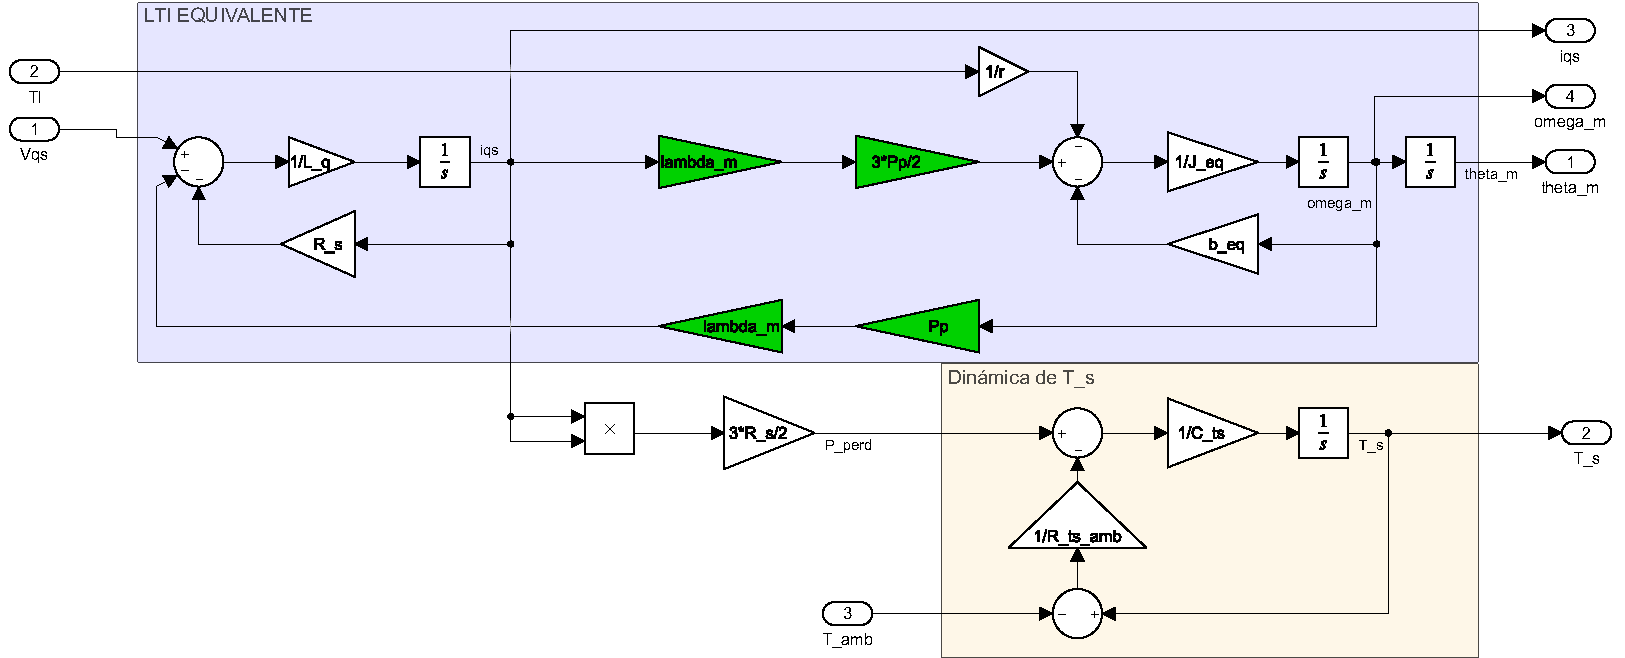
\includegraphics{16-Diagrama_de_bloques_LTI_equivalente_aumentado.pdf}}
    \end{adjustbox}
    \caption{Diagrama de bloques LTI equivalente.}
    \label{diagrama de bloques LTI equivalente}
\end{figure}

\begin{figure}[H]
    \centering
    \begin{adjustbox}{scale=0.8,max width=\columnwidth}
        \framebox{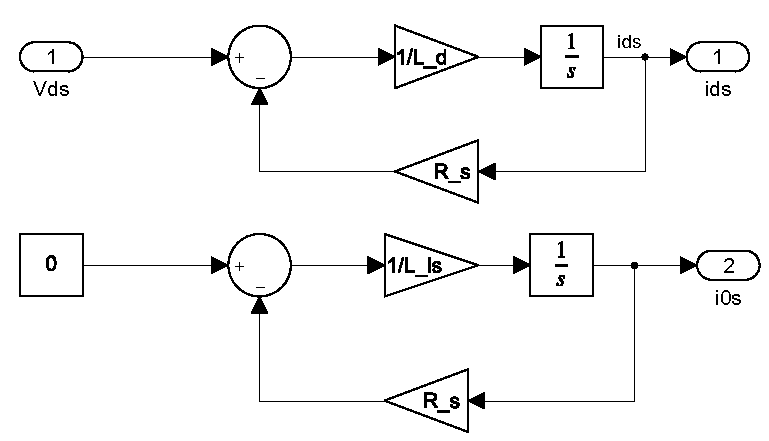
\includegraphics{17-Diagrama_de_bloques_LTI_equivalente_aumentado_i0s_ids.pdf}}
    \end{adjustbox}
    \caption{Dinámica de $i^r_{ds}(t)$ e $i_{0s}(t)$.}
    \label{diagrama de bloques LTI equivalente i0s e ids}
\end{figure}

Para lograr la especificación indicada para $i^r_{ds}(t)$ es necesario realizar una \textbf{Ley de control mínima} que se determina a partir de la ecuación de estado para $i^{r}_{ds}(t)$ (\cref{ecuacion de estado ids}), partiendo de la hipótesis de que $i^{r}_{ds}(0)=0$:

\begin{equation}
	0= \frac{L_q P_p \omega_m(t)i^r_{qs}(t)}{L_d}  + \frac{v^r_{ds}(t)}{L_d}\Rightarrow	v^{r}_{ds}= -L_{q}i^{r}_{qs}(t)P_{p}\omega_{m}(t)\\
	\label{ecuacion determinacion ley de control minima}
\end{equation}

De esta manera queda determinada la ley de control mínima, que debe aplicarse para lograr el desacoplamiento de los canales de flujo magnético y torque.

La \textbf{Implementación}, en el modelo global NL completo, de esta  ley de control mínima, mediante un controlador parcial incorporando el inversor (modulador de tensión trifásico equivalente), las Transformaciones de Park y los sensores de realimentación ideal de variables de estado,
se puede observar en la \cref{Implementación de ley de control mínima}

\begin{figure}[H]
	\centering
	\begin{adjustbox}{scale=0.7,max width=\columnwidth}
		\framebox{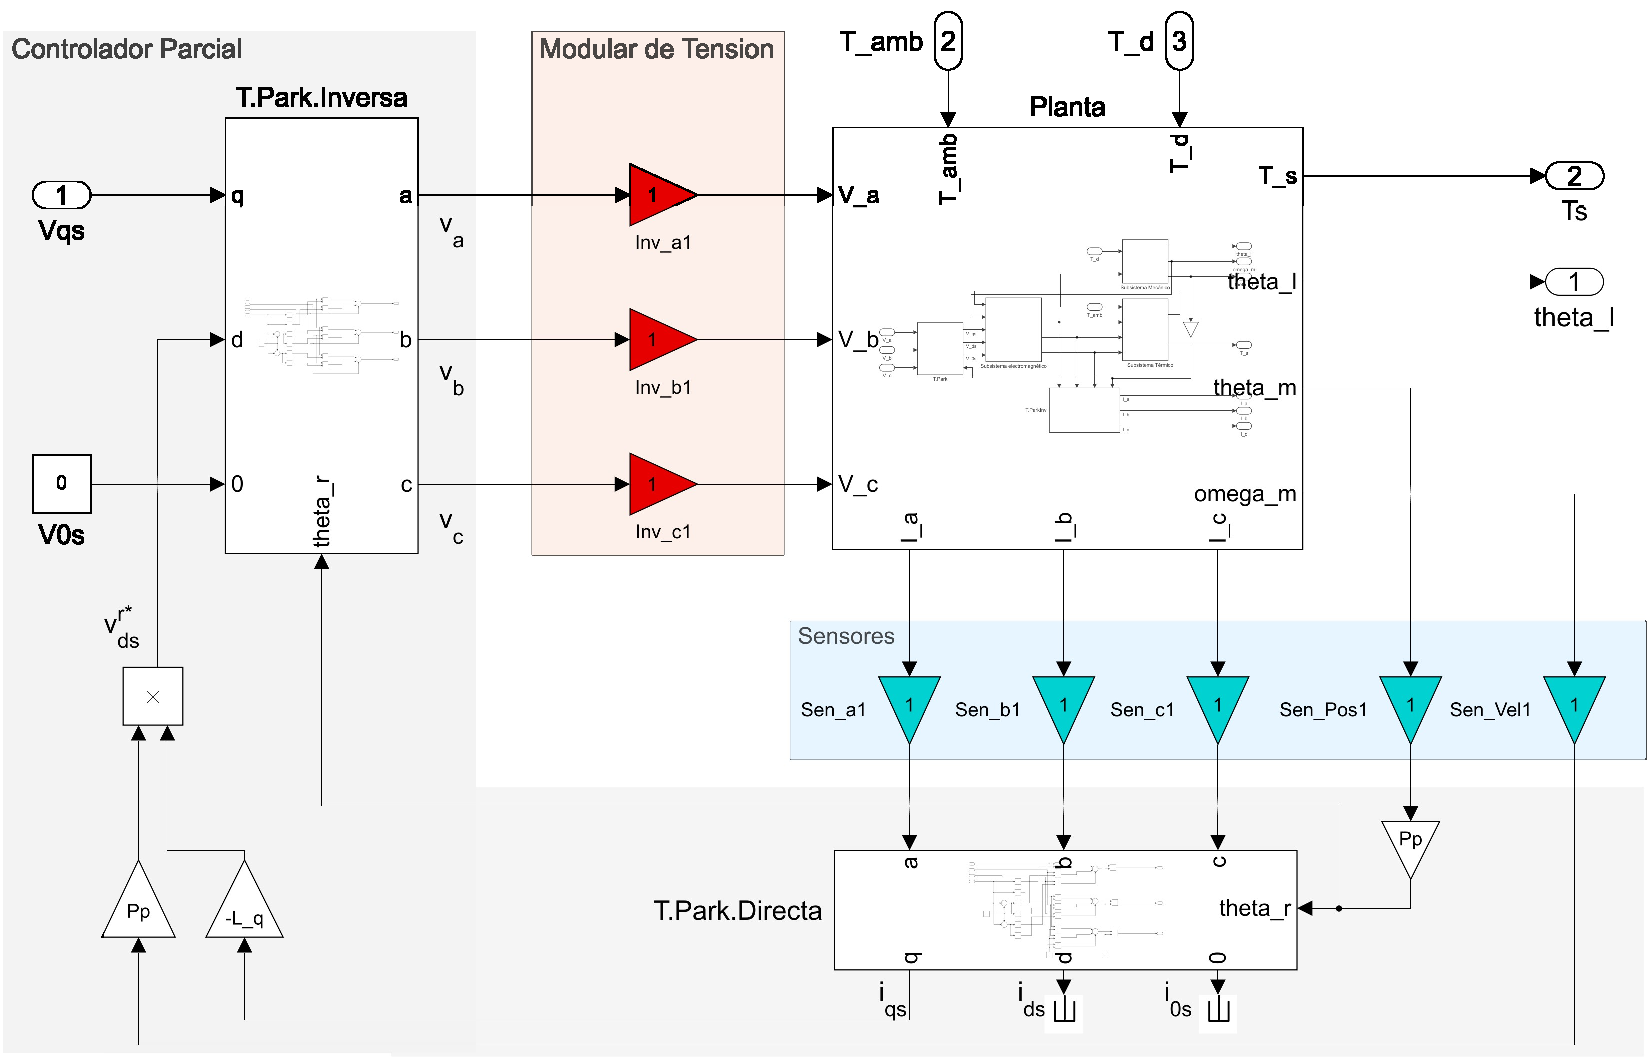
\includegraphics{18-Ley_de_control_minima.pdf}}
	\end{adjustbox}
	\caption{Implementación de ley de control mínima.}
	\label{Implementación de ley de control mínima}
\end{figure}

Para el caso general en donde no se cumple la hipótesis $i^{r}_{ds}(0)=0$, existe una \textbf{dinámica residual} en la corriente $i^{r}_{ds}(t)$. Esta dinámica queda representada con la ecuación diferencial que obtenemos al reemplazar la ley de control mínima (\cref{ecuacion determinacion ley de control minima}) en la \cref{ecuacion de estado ids}:

\begin{equation}
	\frac{d i^r_{ds}(t)}{dt} = -\frac{R_s i^r_{ds}(t)}{L_d} \Rightarrow L_d\frac{d i^r_{ds}(t)}{dt} + R_s i^r_{ds}(t) = 0
	\label{ecuacion dinamica residual ids}
\end{equation}

La cual tiene la siguiente solución:

\begin{equation}
	{i}^r_{ds}(t) = {i}^r_{ds}(0) e^{-\dfrac{R_s}{L_d}t} 
\end{equation}

Como se puede observar  si $i^{r}_{ds}(0)\neq0$, ésta decae exponencialmente hasta llegar a 0. Esto establece un acoplamiento con el eje $q$, produciendo un comportamiento no lineal, que se termina desvaneciendo con el tiempo a medida que $i^{r}_{ds}(t)$ decae. Por lo tanto este fenómeno puede ser despreciado para régimen forzado.

Para evitar esto, se puede implementar una \textbf{ley de control complementaria mínima} sobre el eje $q$, y poder eliminar completamente el acoplamiento residual NL, obteniendo así un modelo equivalente lineal del sistema, aún cuando $i^{r}_{ds}(0)\neq0$. Esto se logró implementando una ley de control que permita deshacerse del término que contiene a $i^{r}_{ds}(t)$ en la \cref{ecuacion de estado iqs}.

\begin{align}
	v^r_{qs}(t) &= L_q\frac{d i^r_{qs}(t)}{dt} + R_s i^r_{qs}(t) +P_p \omega_m(t) \lambda'^r_m +\underline{P_p \omega_m(t) L_d i^r_{ds}(t)} \label{ley de control complementaria 1 }\\
	v^r_{qs}(t) &= v^r_{qs}(t)^{*} + P_p \omega_m(t) L_d i^r_{ds}(t)  \label{ley de control complementaria 2}\\
 	v^r_{qs}(t)^{*} &= L_q\frac{d i^r_{qs}(t)}{dt} + R_s i^r_{qs}(t) +P_p \omega_m(t) \lambda'^r_m  \label{ley de control complementaria 3}
\end{align}

El modelo \textbf{LTI equivalente(incorporando la dinámica residual del eje $\mathbf{d}$)} queda como se indica en la \cref{equaciones modelo LTI eq} y en la \cref{diagrama de bloques modelo LTI eq}. En
las mismas también se incorpora la dinámica asociada a $i_{0s}(t)$ y se actualiza e incorpora la dinámica lineal del sub-sistema térmico, a los efectos de tener un modelo con todas las variables de estado 
para luego poder hacer comparaciones con el modelo LPV (\ref{par: LTI vs LPV}). Sin embargo, los puntos de análisis que se detallan a continuación, y que no implican
comparación con otros moedelos, se realizan con el estado reducido indicado en la \cref{vector de estado reducido}.

\begin{equation}
	\begin{cases}
		\frac{d \theta_m(t)}{dt} = {\omega}_m(t)\\
		\frac{d \omega_m(t)}{dt} = \frac{3}{2} \frac{P_p i^r_{qs}(t)\lambda^{'r}_m}{J_{eq}} - \frac{b_{eq}\omega_m(t)}{J_{eq}} - \frac{T_l(t)}{r J_{eq}}\\
		\frac{d i^r_{qs}(t)}{dt} = -\frac{R_s i^r_{qs}(t)}{L_q} - \frac{P_p \omega_m(t) \lambda^{'r}_m}{L_q}+ \frac{v^r_{qs}(t)}{L_q}\\
		\frac{d i^r_{ds}(t)}{dt} = -\frac{R_s i^r_{ds}(t)}{L_d}	+ v^{r*}_{ds}(t)\\
		\frac{d i_{0s}(t)}{dt} = -\frac{R_s i_{0s}(t)}{L_{ls}}	+ v_{0s}(t)\\
		\frac{d T^\circ_{s}(t)}{dt} = \frac{P_{sperd}(t)}{R_{ts}} + \frac{1}{R_{ts}C_{ts}}\left[T^{\circ}_{amb}(t) - T_{s}^{\circ}(t)\right]
	\end{cases}
	\label{equaciones modelo LTI eq}
\end{equation}

En la \cref{equaciones modelo LTI eq} la $P_{sperd}(t)$ viene dada según la \cref{potencia de perdidas}. También se incorpora la entrada $v^{r*}_{ds}(t)$, que se obtiene al restar a  $v^r_{ds}(t)$
la ley de control mínima. Para el caso que presentamos aquí será $v^{r*}_{ds}(t) \equiv 0$ y $v_{0s}(t) \equiv0 $.


El diagrama de bloques del \textbf{modelo NL desacoplado con ley de control NL} se observa en la \cref{Implementación de ley de control complementaria}

\begin{figure}[H]
	\centering
	\begin{adjustbox}{scale=0.7,max width=\columnwidth}
		\framebox{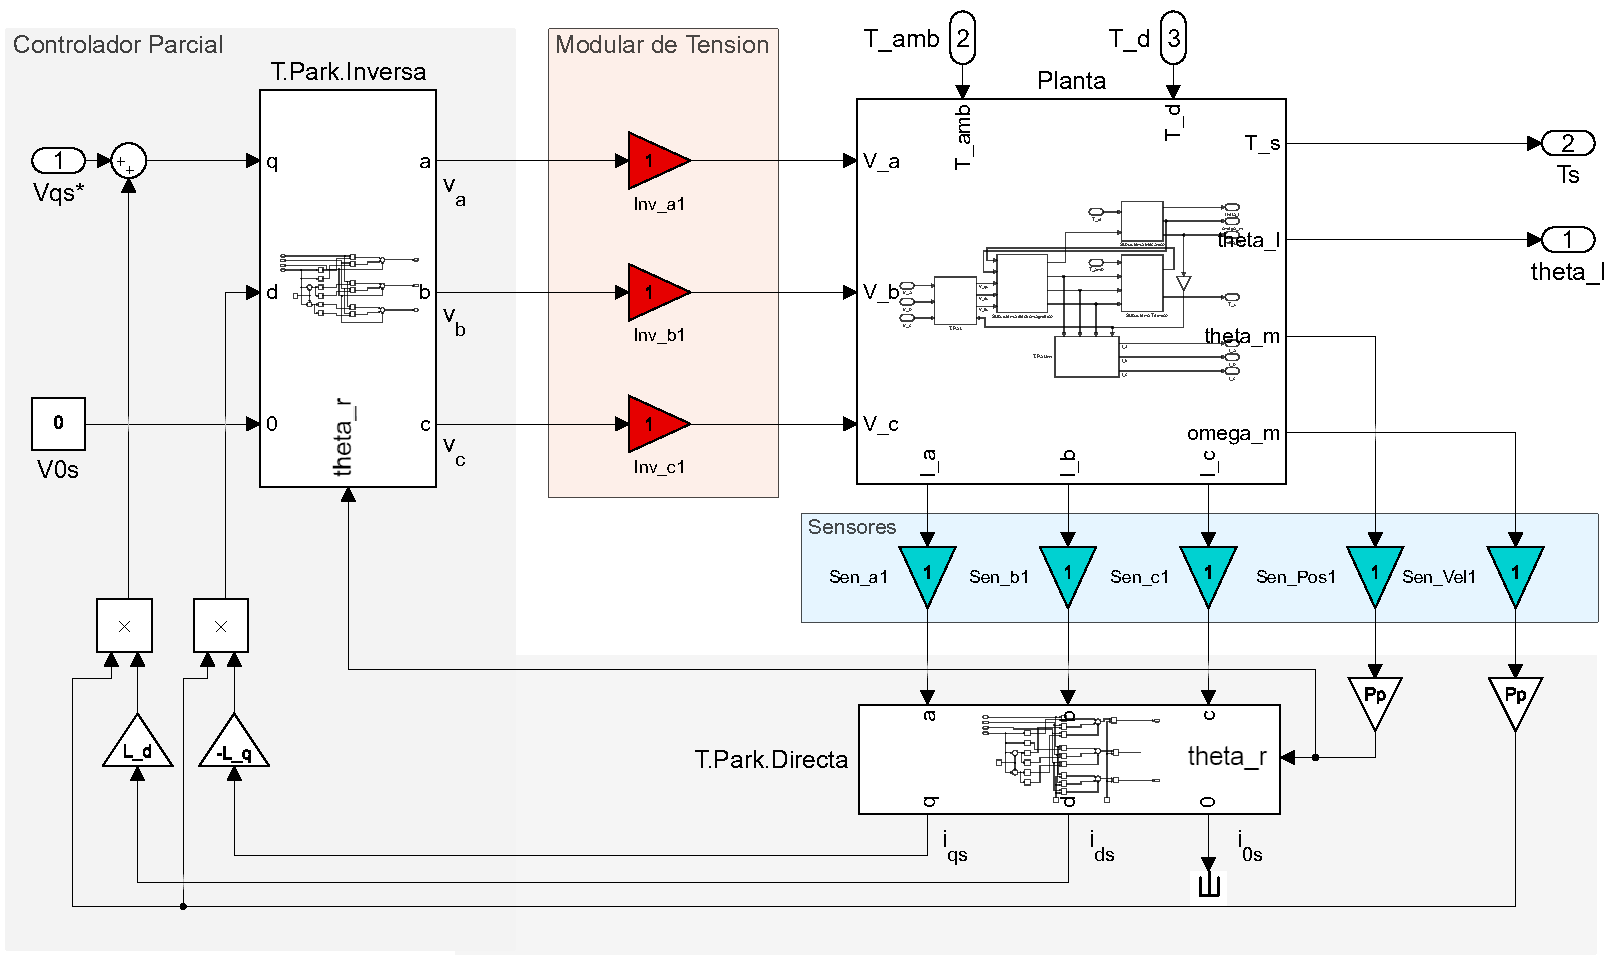
\includegraphics{19-Ley_de_control_complementaria.pdf}}
	\end{adjustbox}
	\caption{Implementación de ley de control complementaria.}
	\label{Implementación de ley de control complementaria}
\end{figure}

\begin{figure}[H]
	\centering
	\begin{adjustbox}{max width=\columnwidth}
		\framebox{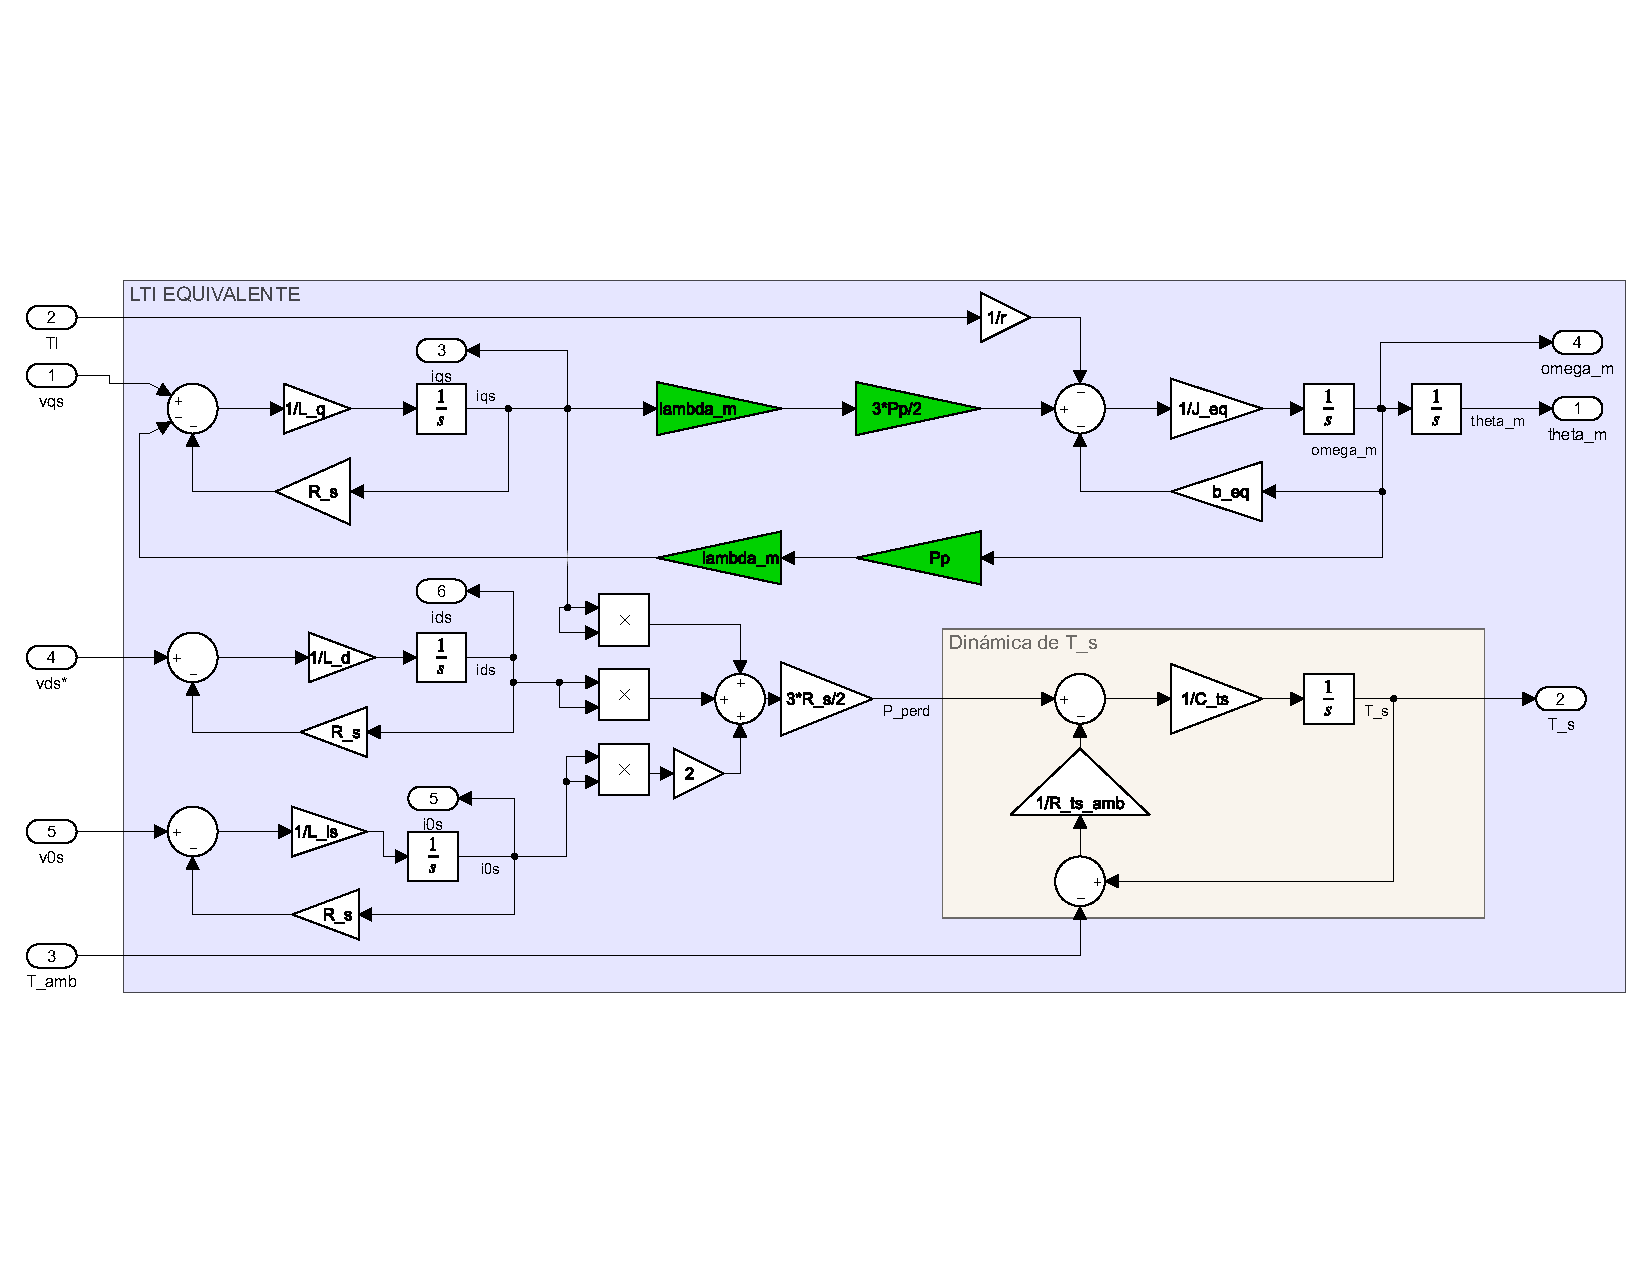
\includegraphics{20-Diagrama_de_bloques_LTI_equivalente_aumentado_dinamica_residual.pdf}}
	\end{adjustbox}
	\caption{Diagrama de bloques LTI equivalente aumentado con dinámica residual eje d.}
	\label{diagrama de bloques modelo LTI eq}
\end{figure}

\paragraph{\textbf{Comparación del modelo dinámico LTI equivalente aumentado vs. el modelo dinámico global LPV}}
En primer lugar, en la \cref{diagrama de bloques LPV} se muestra el diagrama de bloques de estado del sistema LPV, en el que las ganancias $A(i, j)$ y $B(i, j)$
son los correspondientes elementos en las matrices de la \cref{matriz_AB}.
Por otro lado, en la \cref{diagrama de bloques LPV vs LTI} se muestra cómo se realizó la comparación entre los modelos. Como se puede observar en esta última,
incorporamos al modelo LPV los valores de los estados y entradas en el punto de operación.
\label{par: LTI vs LPV}
\begin{figure}[H]
	\centering
	\begin{adjustbox}{max width=\columnwidth}
		\framebox{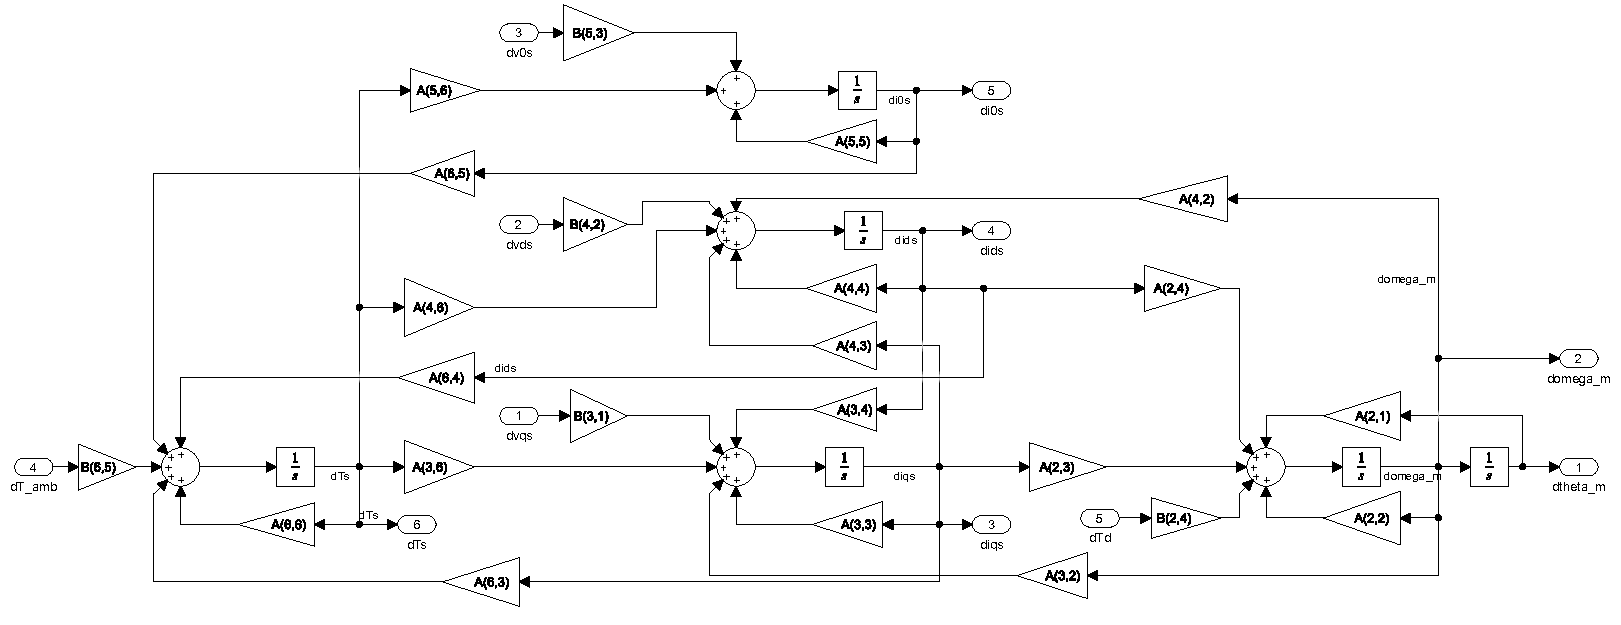
\includegraphics{21-LPV_diagrama_de_bloques.pdf}}
	\end{adjustbox}
	\caption{Diagrama de bloques del modelo LPV.}
	\label{diagrama de bloques LPV}
\end{figure}

\begin{figure}[H]
	\centering
	\begin{adjustbox}{max width=\columnwidth}
		\framebox{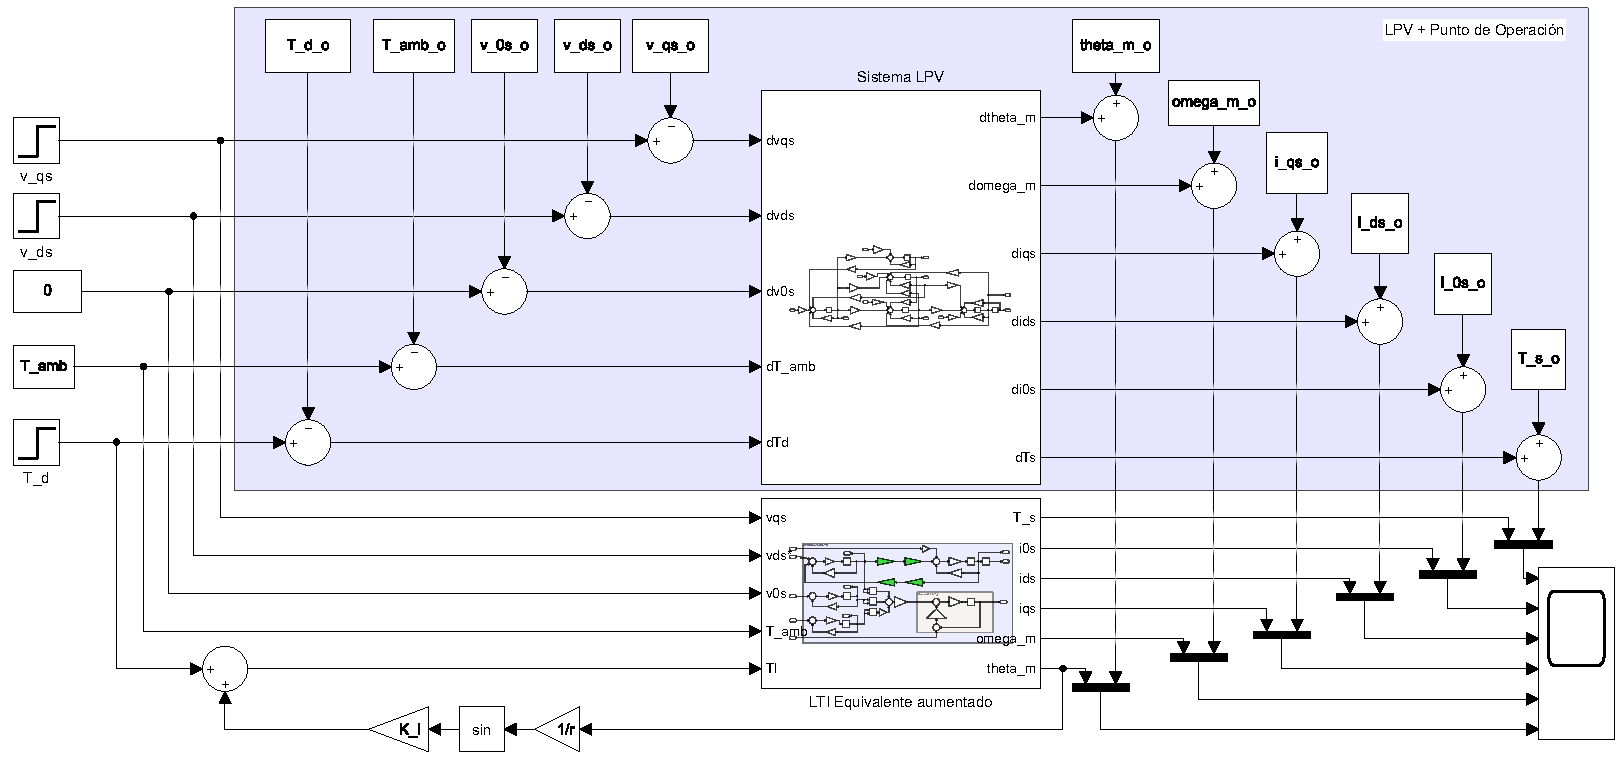
\includegraphics{22-LTI_vs_LPV_diagrama_de_bloques.pdf}}
	\end{adjustbox}
	\caption{Comparación de modelos LTI y LPV diagrama de bloques.}
	\label{diagrama de bloques LPV vs LTI}
\end{figure}

Para la comparación de los modelos primero se definen de forma parcial el vector de entradas y de estado del sistema en el punto de operación,
de modo que el resto de las variables en el punto de operación queden determinadas a partir de la \cref{modelo de operacion NL cuasi_estacionario desarrollado reducido}. Luego se aplican
las mismas entradas a ambos modelos y se comparan los estados en el tiempo.

En todos los casos, las condiciones iniciales son las dadas en la \cref{condiciones iniciales comparación} y se considera para 
el modelo LTI el valor de $R_s$ obtenido para $T^\circ_{s-o}$.

\begin{equation}
	\begin{cases}
		\mathbf{\delta x}(0) &\equiv \mathbf{0}\\
		\mathbf{x}(0) 
		&=
		\begin{bmatrix} 
			0 \\ 
			0 \\ 
			0 \\ 
			0 \\ 
			0 \\ 
			T^\circ_{amb} = 25^\circ C
		\end{bmatrix}
	\end{cases}
	\label{condiciones iniciales comparación}
\end{equation}

Se realizaron 5 simulaciones. Para todas las ellas se tiene 
$\omega_{m-o} \equiv 0\,\left[rad/s\right]$ (solo hay puntos de operación como tal bajo esta condición según
se indicó cuando se analizó el modelo global NL de puntos de operación cuasi-estacionario), $\theta_{m-o}\equiv \frac{r\pi}{12}\,\left[rad\right]$ (esto
es equivalente a desplazar 15° al brazo robótico desde su posición de equilibrio estable), $v_{0s-o} \equiv 0\,\left[V\right]$ (lo que implica $i_{0s-o}\equiv 0\, \left[A\right]$), $T_{d-o} \equiv 1\, \left[N\cdot m\right]$
y $T^\circ_{amb-o}\equiv 25^\circ\, C$.

Para las primeras tres simulaciones se considera además  $v^r_{ds-o}\equiv 0 \,\left[V\right]$ y las entradas son las del punto de operación.
Los resultados de la primera simulación se muestran en las \cref{simulación 1 estado} y \cref{simulación 1 entradas}.
Para la segunda simulación se considera que las entradas se encuentran desviadas respecto de sus valores para el punto de operación y los resultados se muestran
en las \cref{simulación 2 estado} y \cref{simulación 2 entradas}. En la tercera simulación se hizo lo mismo que para la segunda simulación, pero se consideraron desviaciones más
pequeñas, los resultados en las \cref{simulación 3 estado} y \cref{simulación 3 entradas}.



\begin{figure}[H]
	\centering
	\begin{adjustbox}{max width=\columnwidth}
		\framebox{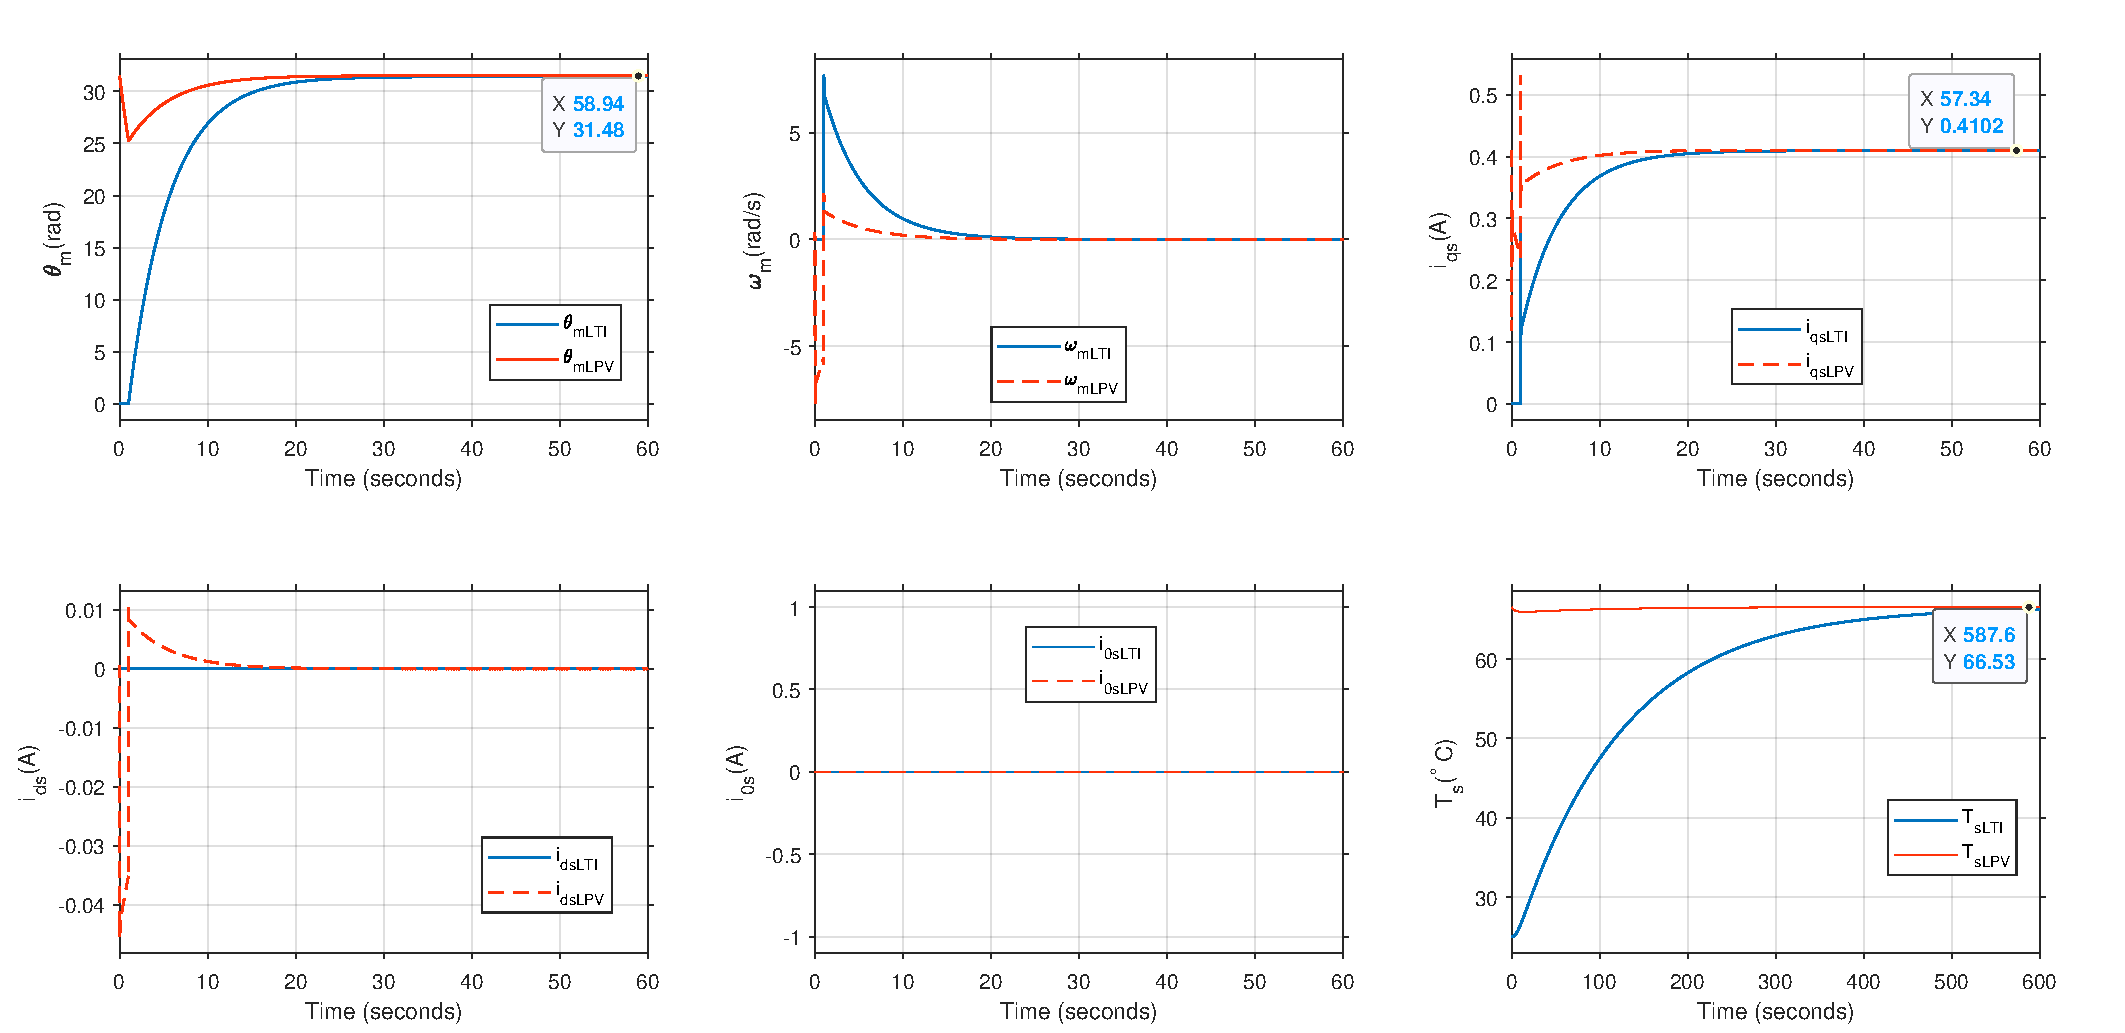
\includegraphics{23-LTI_vs_LPV_simulacion_2.pdf}}
	\end{adjustbox}
	\caption{LTI vs LPV: Simulación 1. Estado. Entradas en el punto de operación.}
	\label{simulación 1 estado}
\end{figure}

\begin{figure}[H]
	\centering
	\begin{adjustbox}{scale=0.6,max width=\columnwidth}
		\framebox{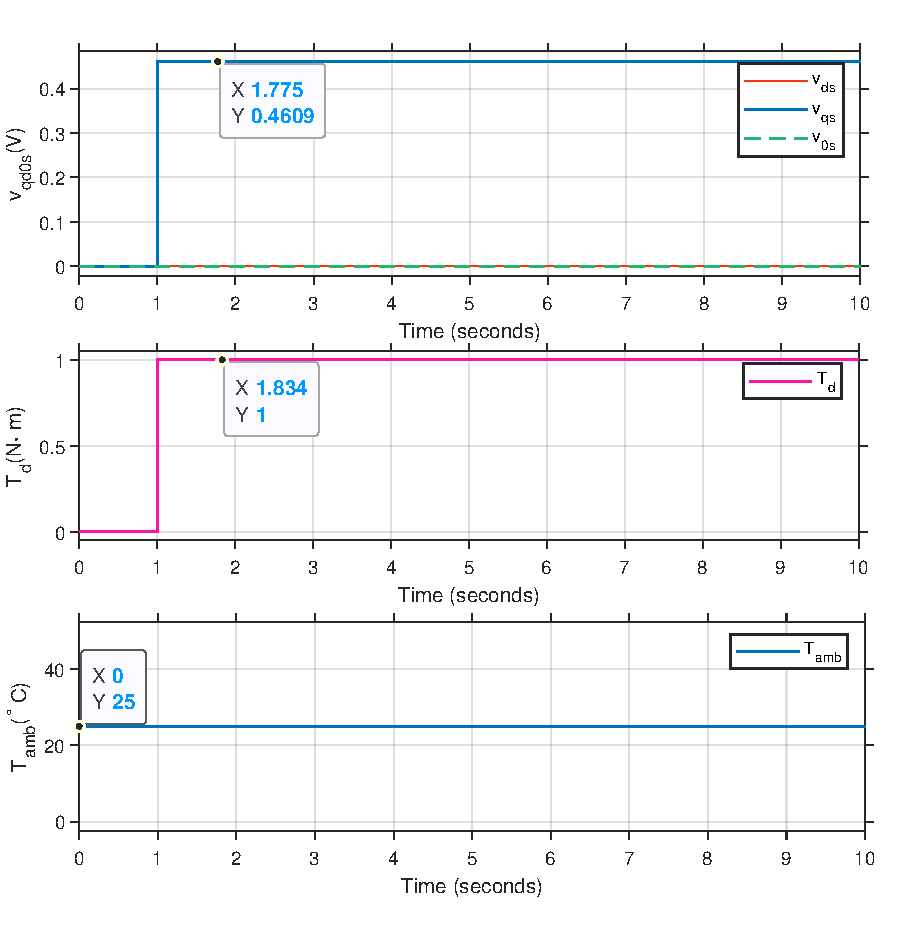
\includegraphics{24-LTI_vs_LPV_simulacion_2_entradas.pdf}}
	\end{adjustbox}
	\caption{LTI vs LPV: Simulación 1. Entradas. Entradas en el punto de operación.}
	\label{simulación 1 entradas}
\end{figure}

\begin{figure}[H]
	\centering
	\begin{adjustbox}{max width=\columnwidth}
		\framebox{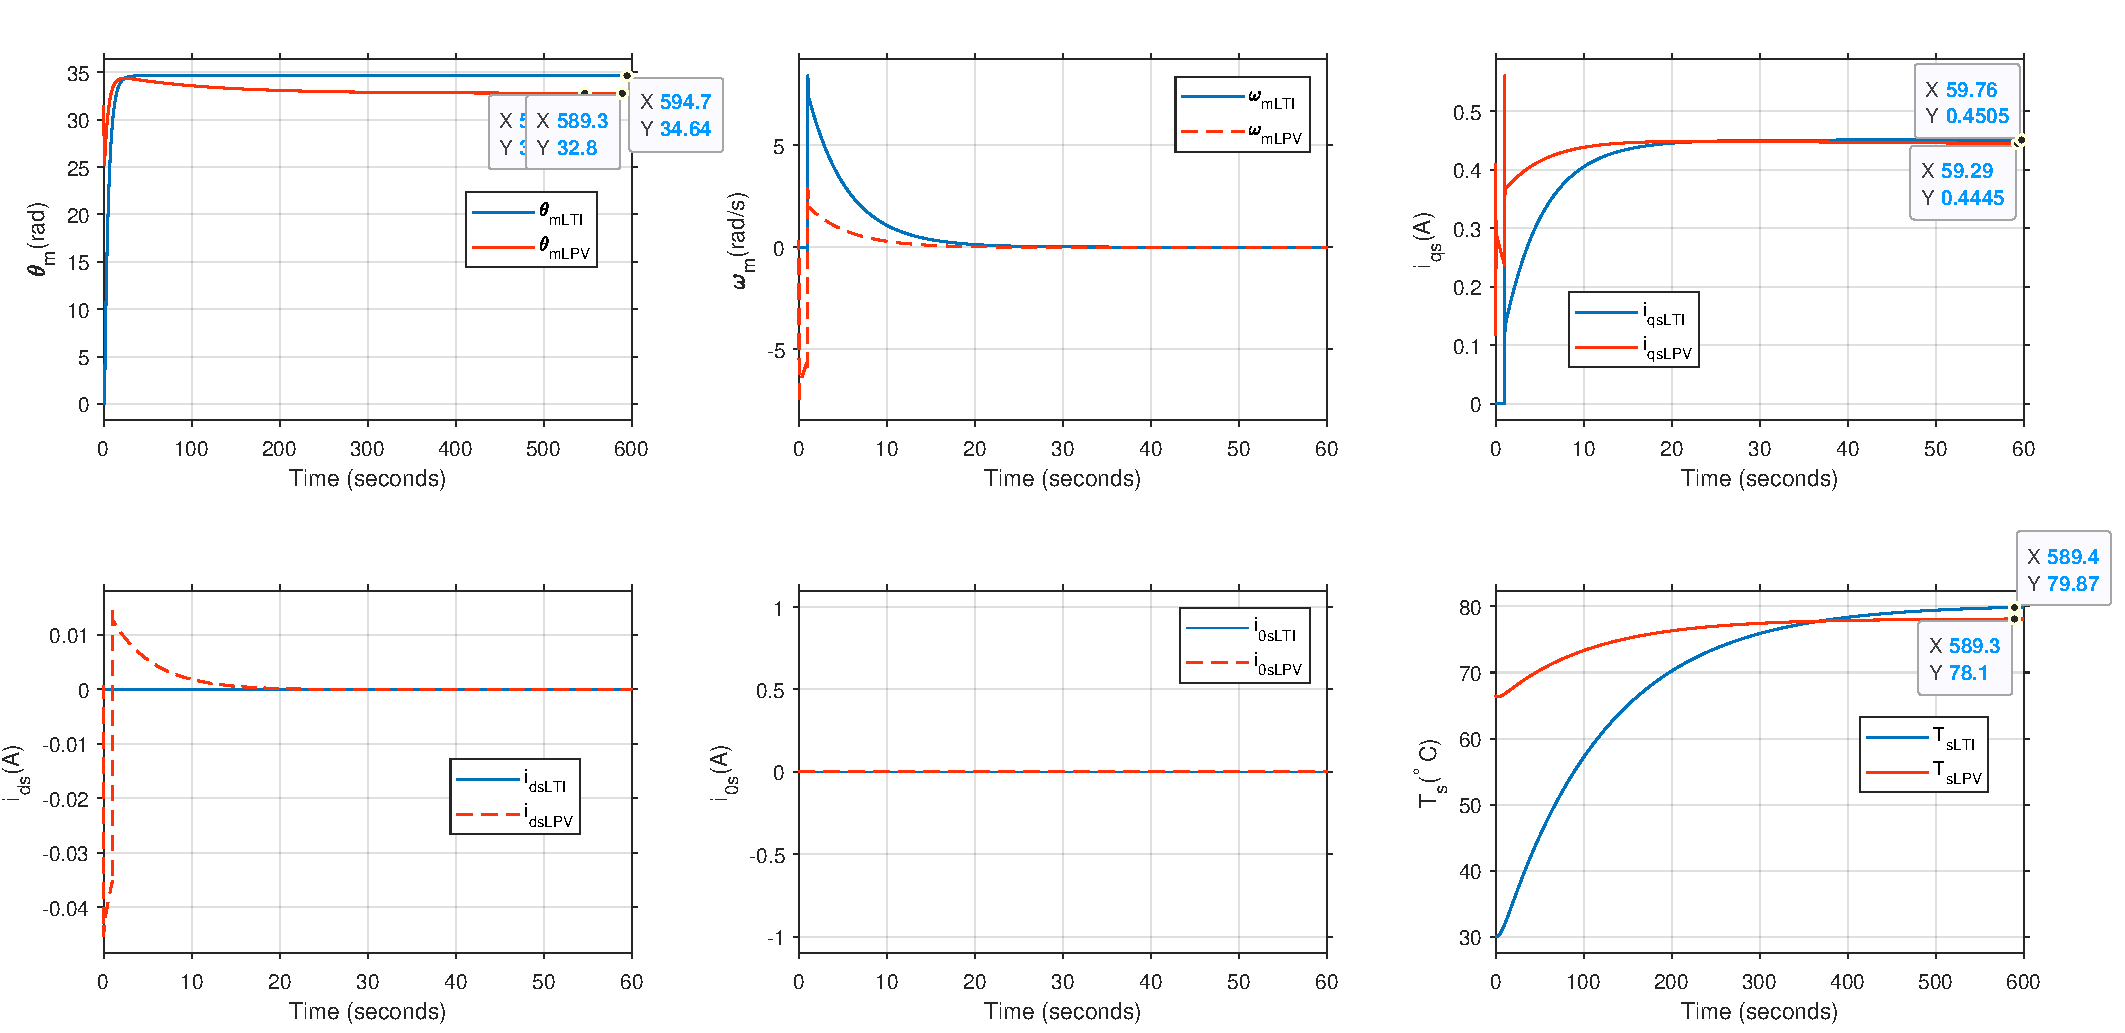
\includegraphics{25-LTI_vs_LPV_simulacion_3.pdf}}
	\end{adjustbox}
	\caption{LTI vs LPV: Simulación 2. Estado. Entradas desviadas del punto de operación.}
	\label{simulación 2 estado}
\end{figure}

\begin{figure}[H]
	\centering
	\begin{adjustbox}{scale=0.7,max width=\columnwidth}
		\framebox{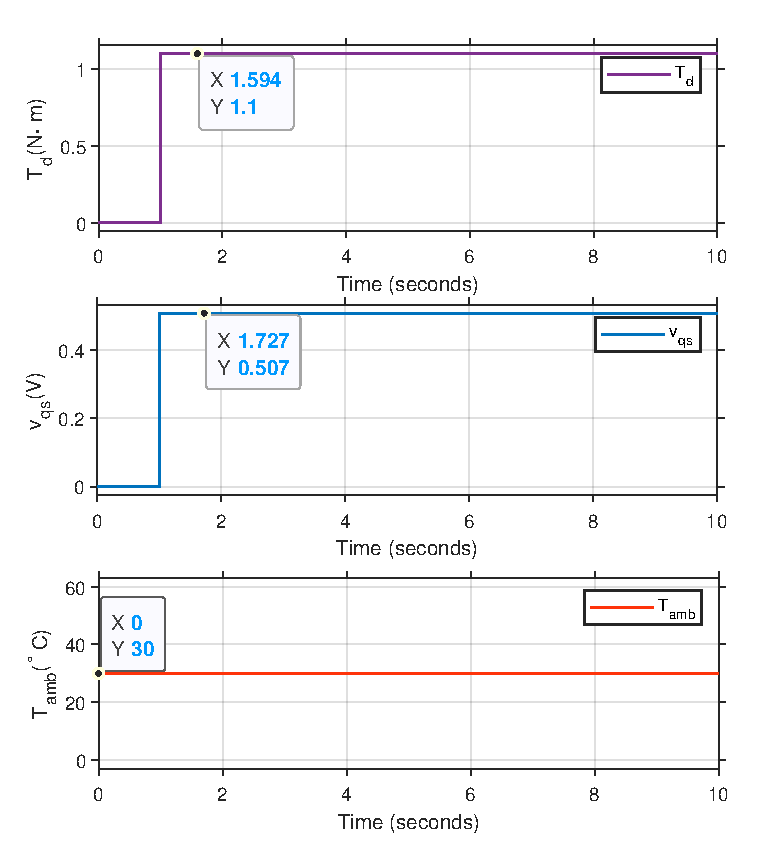
\includegraphics{26-LTI_vs_LPV_simulacion_3_entradas.pdf}}
	\end{adjustbox}
	\caption{LTI vs LPV: Simulación 2. Entradas. Entradas desviadas del punto de operación.}
	\label{simulación 2 entradas}
\end{figure}


\begin{figure}[H]
	\centering
	\begin{adjustbox}{max width=\columnwidth}
		\framebox{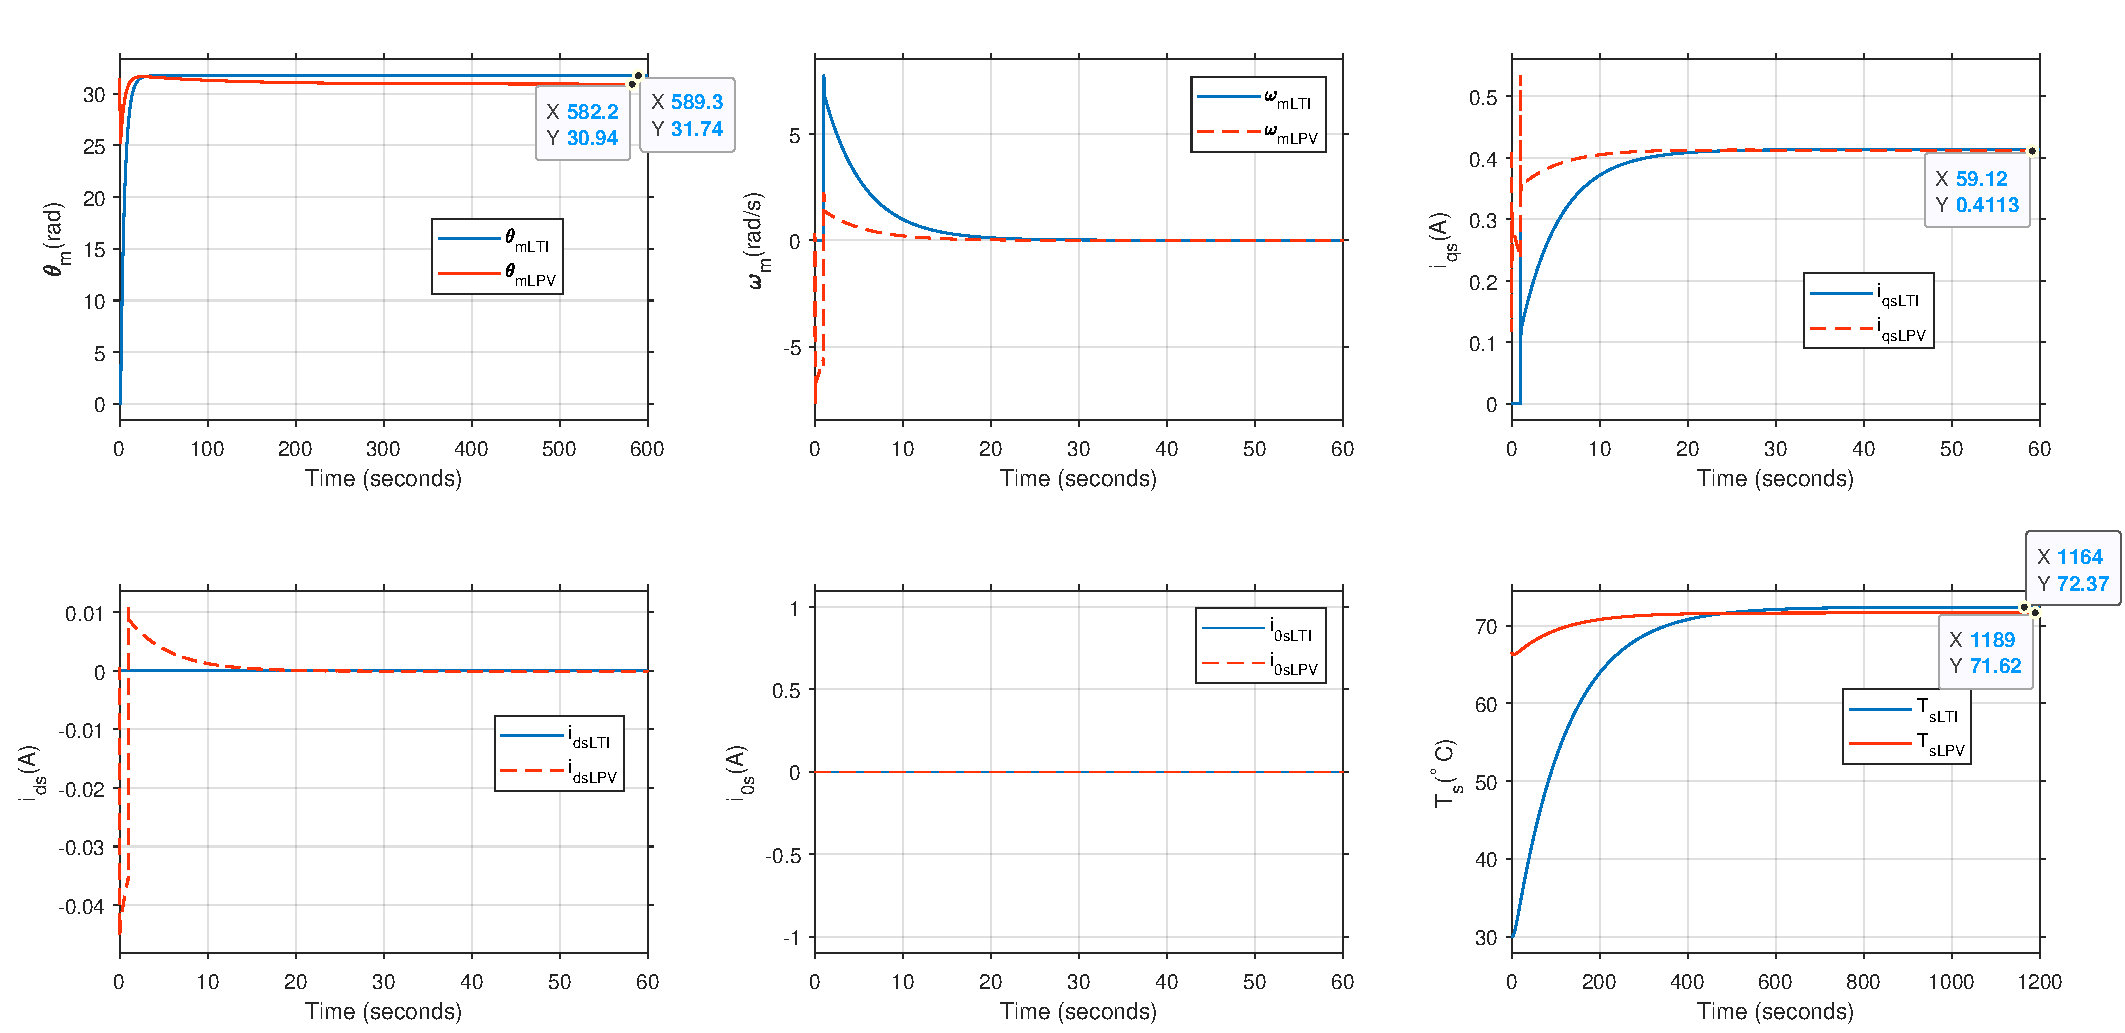
\includegraphics{27-LTI_vs_LPV_simulacion_3_1.pdf}}
	\end{adjustbox}
	\caption{LTI vs LPV: Simulación 3. Estado. Entradas desviadas del punto de operación, menor desviación.}
	\label{simulación 3 estado}
\end{figure}

\begin{figure}[H]
	\centering
	\begin{adjustbox}{scale=0.7,max width=\columnwidth}
		\framebox{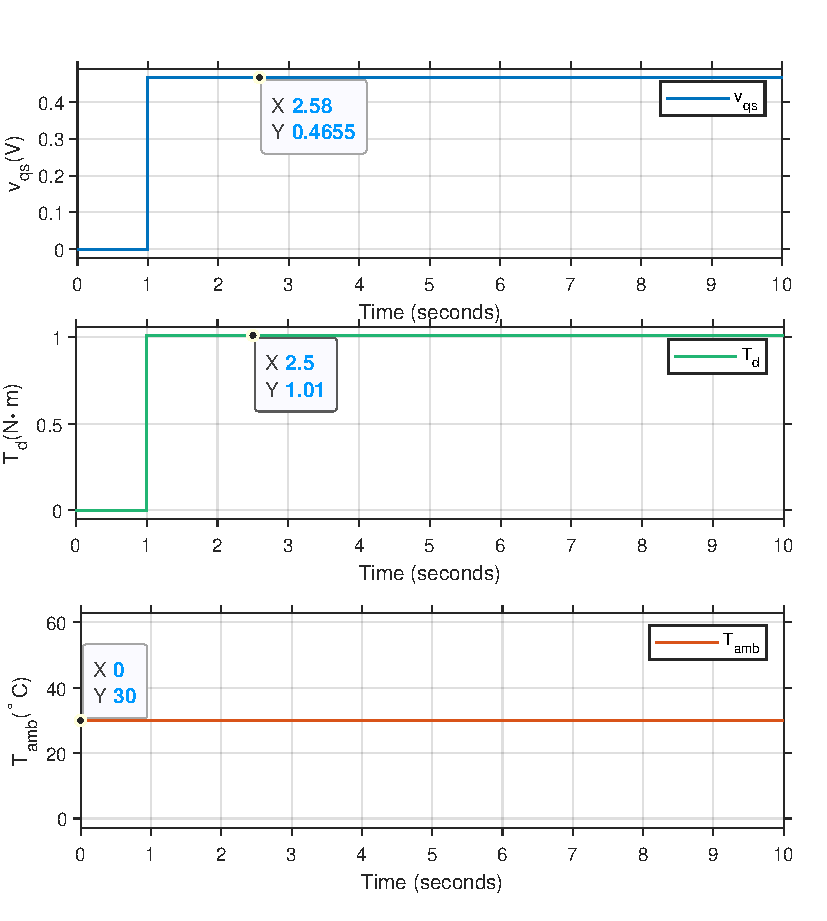
\includegraphics{28-LTI_vs_LPV_simulacion_3_1_entradas.pdf}}
	\end{adjustbox}
	\caption{LTI vs LPV: Simulación 3. Entradas. Entradas desviadas del punto de operación, menor desviación.}
	\label{simulación 3 entradas}
\end{figure}

Para las simulaciones 4 y 5 se evalúa el efecto del reforzamiento/debilitamiento de campo y por eso no se impone $v^r_{ds-o} \equiv 0\, \left[V\right]$.
En cambio, se establece que en el punto de operación, la corriente total en el plano $qd$ (suma vectorial de $i^r_{qs-o}$ e $i^r_{ds-o}$ ) formará un ángulo $\beta = 80^\circ$ con el eje d y habrá reforzamiento de campo,
mientras que para la simulación 5 se considera  $\beta = 100^\circ$ y se consigue debilitamiento de campo. Los resultados
de la simulación 4 se muestran en las \cref{simulación 4 estado}  y \cref{simulación 4 entradas}, y los de las simulación 5 en las \cref{simulación 5 estado} y \cref{simulación 5 entradas}.  En ambos casos las entradas son las del punto de operación.

\begin{figure}[H]
	\centering
	\begin{adjustbox}{max width=\columnwidth}
		\framebox{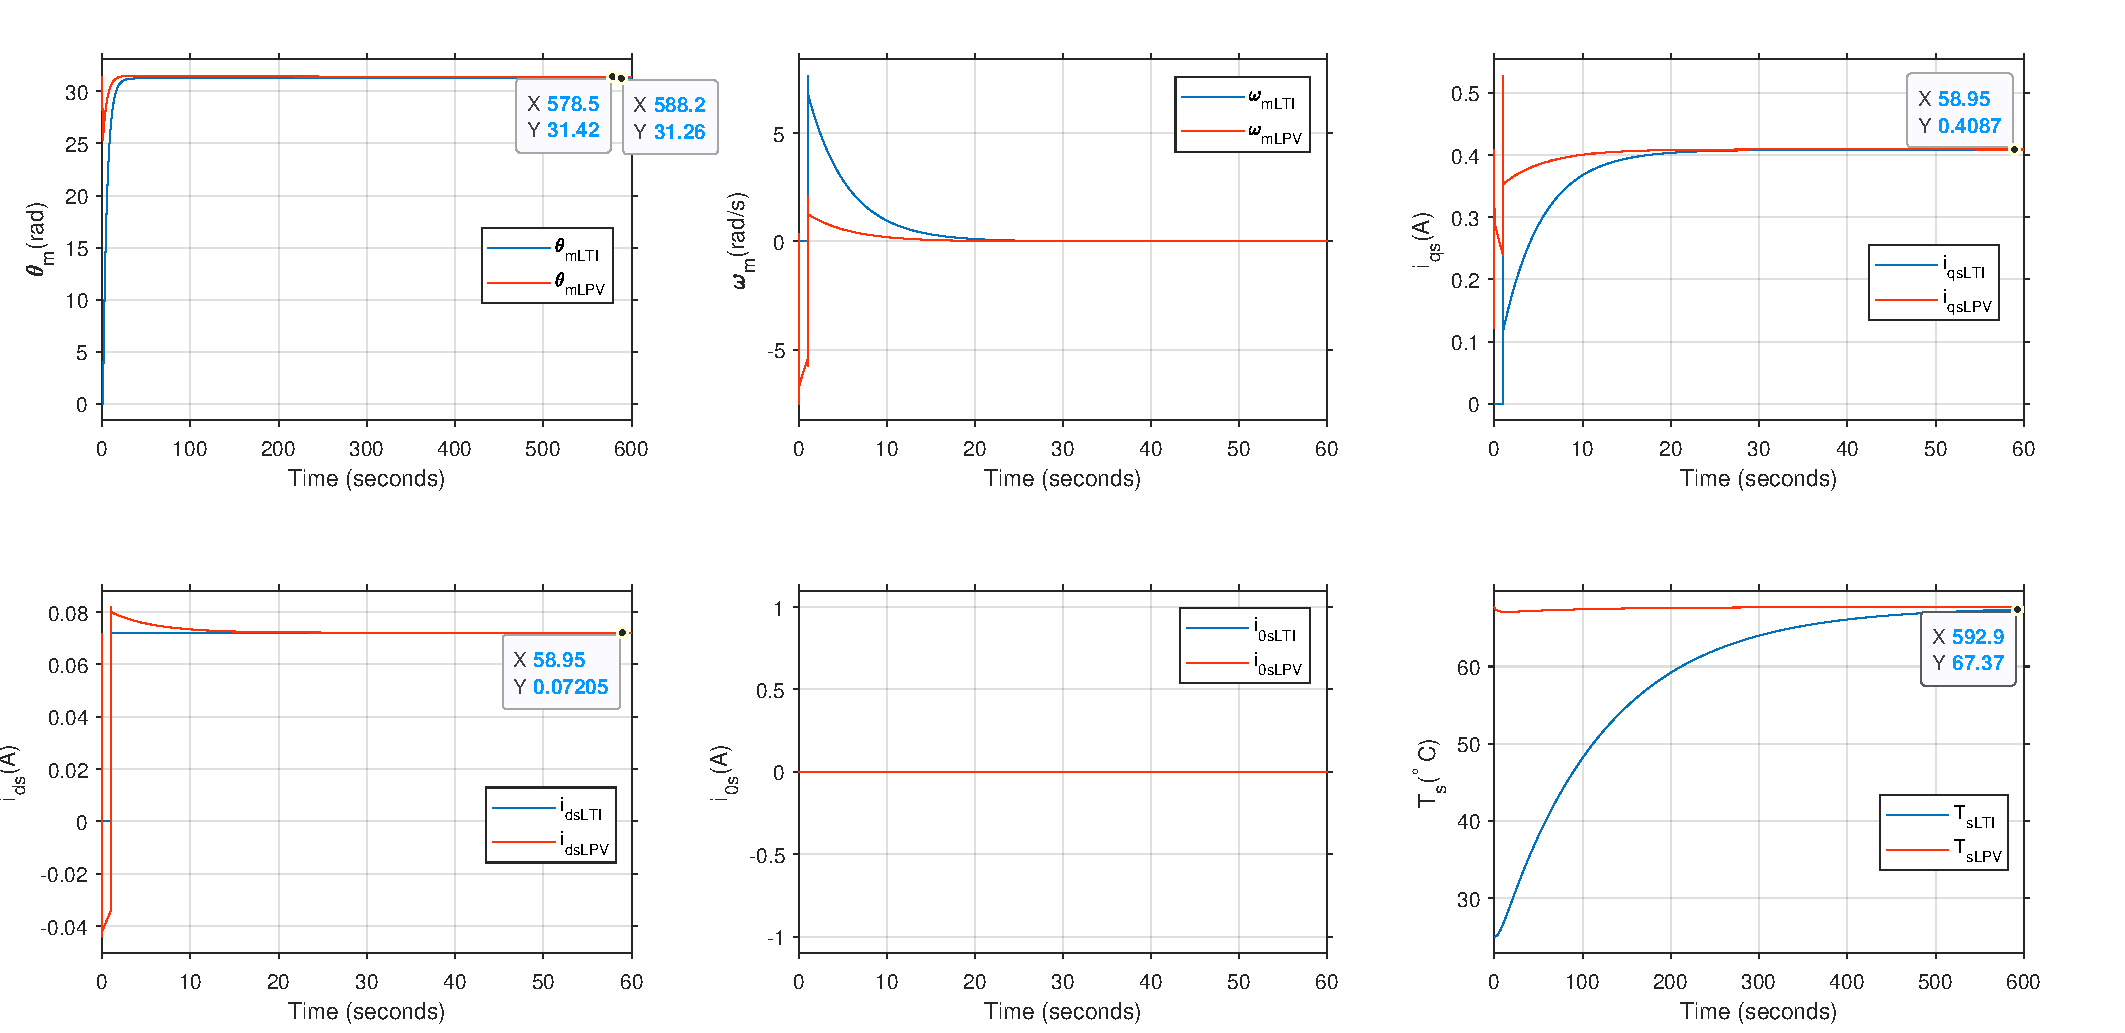
\includegraphics{29-LTI_vs_LPV_simulacion_4_1.pdf}}
	\end{adjustbox}
	\caption{LTI vs LPV: Simulación 4. Estado. Entradas en el punto de operación. Reforzamiento de campo.}
	\label{simulación 4 estado}
\end{figure}

\begin{figure}[H]
	\centering
	\begin{adjustbox}{scale=0.7,max width=\columnwidth}
		\framebox{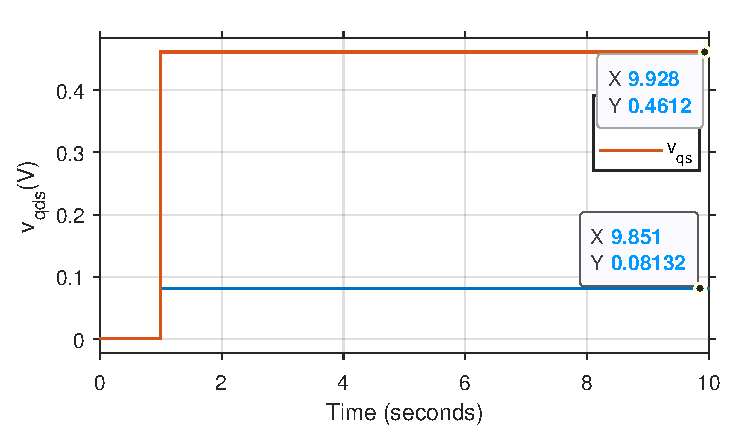
\includegraphics{30-LTI_vs_LPV_simulacion_4_1_entradas.pdf}}
	\end{adjustbox}
	\caption{LTI vs LPV: Simulación 4. Entradas. Entradas en el punto de operación. Reforzamiento de capo}
	\label{simulación 4 entradas}
\end{figure}

\begin{figure}[H]
	\centering
	\begin{adjustbox}{max width=\columnwidth}
		\framebox{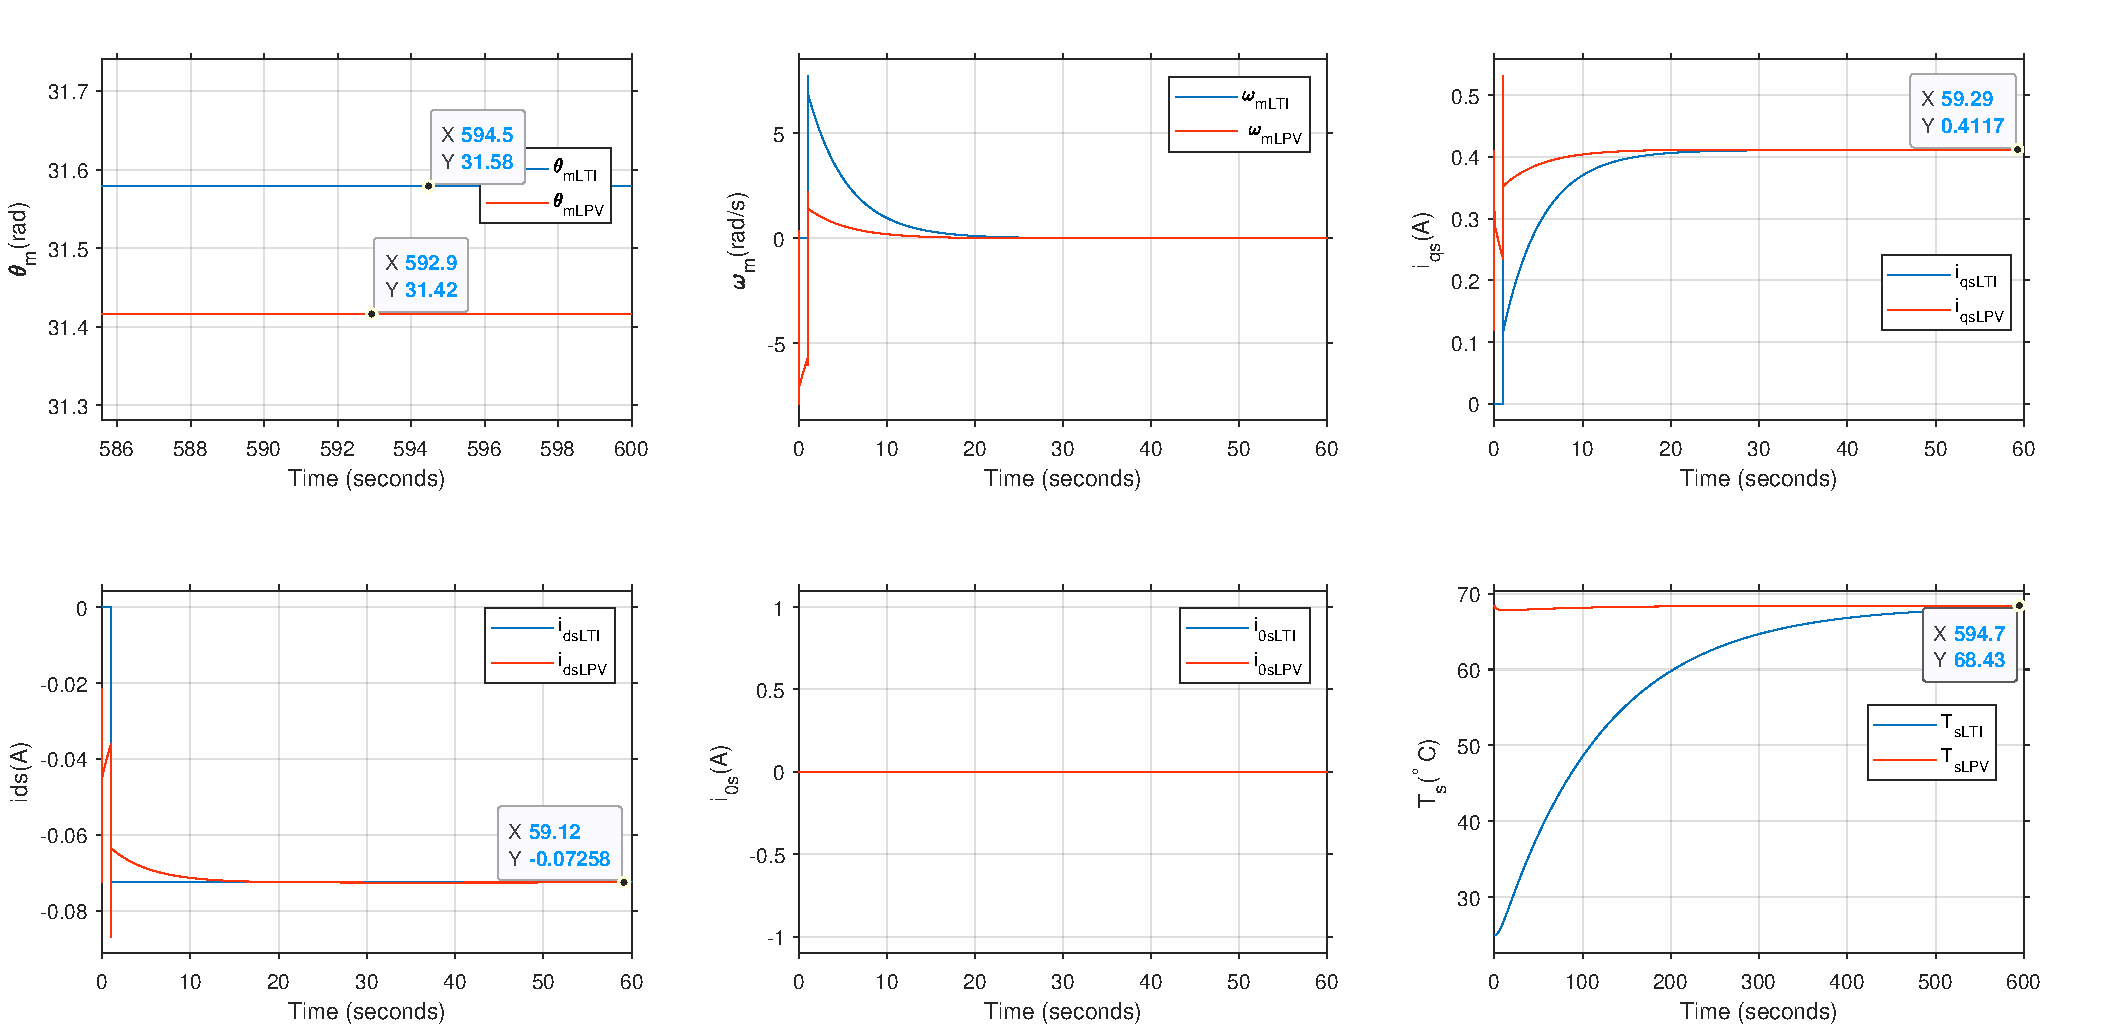
\includegraphics{31-LTI_vs_LPV_simulacion_4_2.pdf}}
	\end{adjustbox}
	\caption{LTI vs LPV: Simulación 5. Estado. Entradas en el punto de operación. Debilitamiento de campo.}
	\label{simulación 5 estado}
\end{figure}

\begin{figure}[H]
	\centering
	\begin{adjustbox}{scale=0.7,max width=\columnwidth}
		\framebox{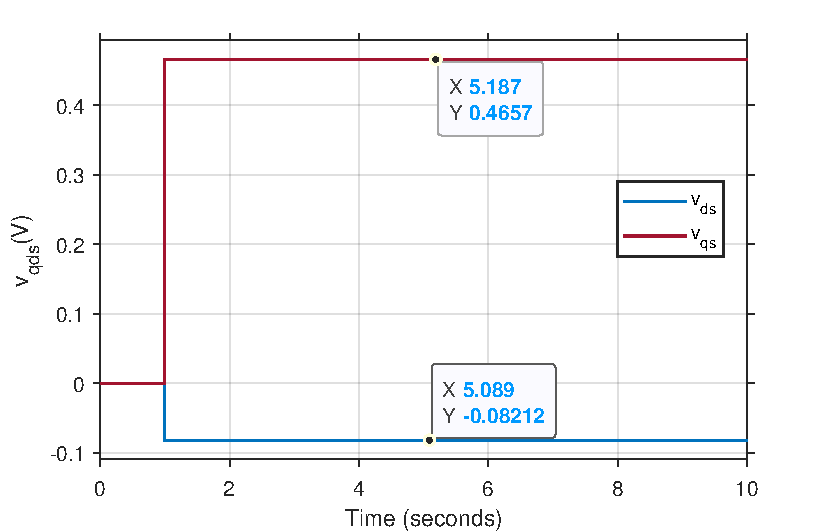
\includegraphics{32-LTI_vs_LPV_simulacion_4_2_entradas.pdf}}
	\end{adjustbox}
	\caption{LTI vs LPV: Simulación 5. Entradas. Entradas en el punto de operación. Debilitamiento de campo.}
	\label{simulación 5 entradas}
\end{figure}

Se puede observar que los modelos tienen un comportamiento
similar en estado permanente aún cuando existe debilitamiento o reforzamiento de campo, el que no es tenido en cuenta
en el modelo LTI al haberse suprimido la contribución de la $i^r_{ds}(t)$ en el torque electromagnético.
En cambio, sí se presentan diferencias más notables en estado permanente cuando las entradas difieren de las correspondientes al 
punto de operación para el cuál se ha obtenido el modelo LPV.


\paragraph{\textbf{Funciones de Transferencia}}
para el modelo LTI equivalente aumentado, desde ambas entradas $V^r_{qs}(s)$ y $T_l(s)$ hacia la salida ${\Theta}_m(s)$.

Primero se aplicó la Transformada de Laplace a la ecuaciones del sistema LTI equivalente aumentado, considerando condiciones iniciales nulas:

\begin{equation}
	\begin{cases}
		s{\Theta}_m(s) = {\Omega}_m(s)\\
		s{\Omega}_m(s) = \frac{3}{2} \frac{P_p I^r_{qs}(s)\lambda^{'r}_m}{J_{eq}} - \frac{b_{eq}\Omega_m(s)}{J_{eq}} - \frac{T_l(s)}{r J_{eq}}\\
		s{I}^r_{qs}(s) = -\frac{R_s I^r_{qs}(s)}{L_q} - \frac{P_p \Omega_m(s) \lambda^{'r}_m}{L_q}+ \frac{V^r_{qs}(s)}{L_q}	
	\end{cases}
	\label{equaciones modelo LTI eq en s}
\end{equation}

Luego se despejó la salida en función de las entradas, para obtener finalmente las funciones de transferencia:

\begin{align}
	{\Theta}_m(s) &= -\frac{R_{s} \frac{T_l(s)}{r} + L_{q} \frac{T_l(s)}{r} s - \dfrac{3}{2} P_{p} V^r_{qs}(s) \lambda^{'r}_m}{J_{eq} L_{q} s^3 +\left( J_{eq} R_{s} + L_{q} b_{eq} \right)s^2 + \left( R_{s} b_{eq} + \dfrac{3}{2} {P_{p}}^2 { \lambda^{'r}_m}^2\right) s}\label{posicion en funcion de demas variables en laplace}\\
	G_{V^r_{qs}}(s) &= \frac{{\Theta}_m(s)}{V^r_{qs}(s)} = \frac{\dfrac{3}{2} P_{p} \lambda^{'r}_m}{J_{eq} L_{q} s^3 +\left( J_{eq} R_{s} + L_{q} b_{eq} \right)s^2 + \left( R_{s} b_{eq} + \dfrac{3}{2} {P_{p}}^2 { \lambda^{'r}_m}^2\right) s}\label{funcion de transferencia desde Vqs}\\
	G_{T_l}(s) &= \frac{{\Theta}_m(s)}{T_l(s)} = -\frac{\frac{1}{r}\left( R_{s} + L_{q} s\right) }{J_{eq} L_{q} s^3 +\left( J_{eq} R_{s} + L_{q} b_{eq} \right)s^2 + \left( R_{s} b_{eq} + \dfrac{3}{2} {P_{p}}^2 { \lambda^{'r}_m}^2\right) s}
	\label{funcion de transferencia desde T_l}
\end{align}

\subsubsection{\textbf{Análisis de estabilidad a lazo abierto para el modelo LTI equivalente aumentado}}
\paragraph{\textbf{Determinación de polos y ceros del sistema}}
Para determinar los polos, se resolvió el polinomio característico del sistema:

\begin{equation}
	J_{eq} L_{q} s^3 +\left( J_{eq} R_{s} + L_{q} b_{eq} \right)s^2 + \left( R_{s} b_{eq} + \dfrac{3}{2} {P_{p}}^2 { \lambda^{'r}_m}^2\right) s = 0
    \label{polinomio caracteristico del sistema LTI}
\end{equation}

Cuyas soluciones fueron indicadas en la \cref{polos del sistema LTI} junto con sus valores
para los parámetros nominales de la carga.
En donde el polo en el origen está asociado al integrador puro a la salida
del sistema, correspondiente con
el pseudo-estado $\theta_m(t)$. Sin considerar este polo, se tiene un sistema de
segundo orden, como lo ponen de manifiesto los dos integradores asociados a $i^r_{qs}(t)$ en el
sub-sistema electromagnético y el asociado a $\omega_m(t)$ en el sub-sistema mecánico.

\begin{equation}
	\begin{cases}
		s_1 = 0\\
		s_2 = \frac{-\left( L_{q} b_{eq} + J_{eq} R_{s}\right)  + \sqrt{{J_{eq}}^2 {R_{s}}^2 - 6 J_{eq} L_{q} {P_{p}}^2 {\lambda^{'r}_m}^2 - 2 J_{eq} L_{q} R_{s} b_{eq}+{L_{q}}^2 {b_{eq}}^2} }{2 J_{eq} L_{q}} = \left(-77.8+\mathrm{i} \, 143.5 = 163.2 \, e^{\mathrm{i} \, 2.07}\right)\left[\frac{rad}{s}\right]\\
		s_3 = \frac{-\left( L_{q} b_{eq} + J_{eq} R_{s}\right)  - \sqrt{{J_{eq}}^2 {R_{s}}^2 - 6 J_{eq} L_{q} {P_{p}}^2 {\lambda^{'r}_m}^2 - 2 J_{eq} L_{q} R_{s} b_{eq}+{L_{q}}^2 {b_{eq}}^2} }{2 J_{eq} L_{q}} = \left(-77.8-\mathrm{i} \, 143.5 = 163.2 \, e^{-\mathrm{i} \, 2.07}\right)\left[\frac{rad}{s}\right]
	\end{cases}\label{polos del sistema LTI}
\end{equation}

Además, se obtuvieron las expresiones de la frecuencia natural (\cref{ecuacion de las frecuencias naturales del LTI}) y relación de amortiguamiento crítico (\cref{ecuacion de las relaciones de amortiguamiento del LTI}), junto con sus valores
para los parámetros nominales al comparar la ecuación característica asociada a los dos polos complejos conjugados (\cref{polinomio caracteristico del sistema LTI polos complejos conjugados}), con  la ecuación estándar de un sistema de segundo orden sub-amortiguado (\cref{ecuación estandar de un sistema de segundo orden}).

\begin{align}
	s^2 +\dfrac{ J_{eq} R_{s} + L_{q} b_{eq}}{J_{eq} L_{q}} &s +\dfrac{ R_{s} b_{eq} + \dfrac{3}{2} {P_{p}}^2 { \lambda^{'r}_m}^2}{J_{eq} L_{q}}  = 0 \label{polinomio caracteristico del sistema LTI polos complejos conjugados}\\
	s^2 + 2 \zeta \omega_{n} &s + \omega_{n}^{2} = 0 \label{ecuación estandar de un sistema de segundo orden}
\end{align}

\begin{align}
	\omega_{n} &= \sqrt{\dfrac{ R_{s} b_{eq} + \dfrac{3}{2} {P_{p}}^2 { \lambda^{'r}_m}^2}{J_{eq} L_{q}}} = 163.2 \left[\frac{rad}{s}\right] \label{ecuacion de las frecuencias naturales del LTI}\\
	\zeta &= \dfrac{ J_{eq} R_{s} + L_{q} b_{eq}}{2 \sqrt{ J_{eq} L_{q}\left( R_{s} b_{eq} + \dfrac{3}{2} {P_{p}}^2 { \lambda^{'r}_m}^2\right) }} = 0.4868 \label{ecuacion de las relaciones de amortiguamiento del LTI}
\end{align}

Se pudo ver que solo la perturbación introduce un cero:

\begin{align}
	R_{s} + L_{q} s = 0 \Rightarrow s = -\frac{R_{s}}{L_{q}} = -154.54 \left[\frac{rad}{s}\right]
	\label{cero del sistema LTI}
\end{align}


Luego se quiere evaluar la variación de  polos, frecuencia natural y  cero ante la 
\textbf{migración de propiedades} del sistema debida a la variación de los parámetros de la carga
$J_l$ y $b_l$ \cite{c1}. Resulta de interés, también conocer la migración
de propiedades ante el cambio de $R_s$ al considerar temperaturas de equilibrio en los extremos del rango de operación.
%aca vendría a la cita en la guía donde dice lo de la variación de parametros.

Al trazar el mapa de polos y ceros del sistema se puede observar que
los polos complejos conjugados presentan poca variación relativa ante el cambio de $b_l$ en comparación con la variación ante el cambio de $J_l$ y de $R_s$.
Por este motivo, en la \cref{mapa de polos b_l nominal} se presenta, por un lado, el mapa de polos y ceros completo cuando
$b_l = b_{lnom} = 0.1 \left[\frac{N \cdot m}{rad \cdot s}\right]$ y $J_l$ varía en todo su rango con $R_s$ a $-15^\circ C$, a $40^\circ C$ y a $115^\circ C$. Mientras que en la
\cref{mapa de polos complejos} se muestra solo el mapa de los polos complejos cuando
$b_l$ toma cinco valores equi-espaciados en su rango, y para cada uno, $J_l$ varía en todo su rango ($R_s$ solo a $40^\circ C$).
En estas figuras se indica con $max J_{l}$ y $min J_{l} = J_{lnom}$ a los polos correspondientes al máximo y mínimo valor
de $J_{l}$ respectivamente. Luego, en cada curva, $J_l$ varía desde un mínimo a un máximo
desde la parte superior izquierda de la gráfica hacia la parte inferior derecha de la misma. Es decir, como se espera, 
el aumento de $J_{l}$  produce un correspondiente incremento en $J_{eq}$,
lo que a su vez produce una disminución de la frecuencia natural $\omega_n$ asociada a los polos complejos sin un apreciable
cambio en el amortiguamiento del sistema.

\begin{figure}[H]
	\centering
	\begin{adjustbox}{scale=0.7,max width=\columnwidth}
		\framebox{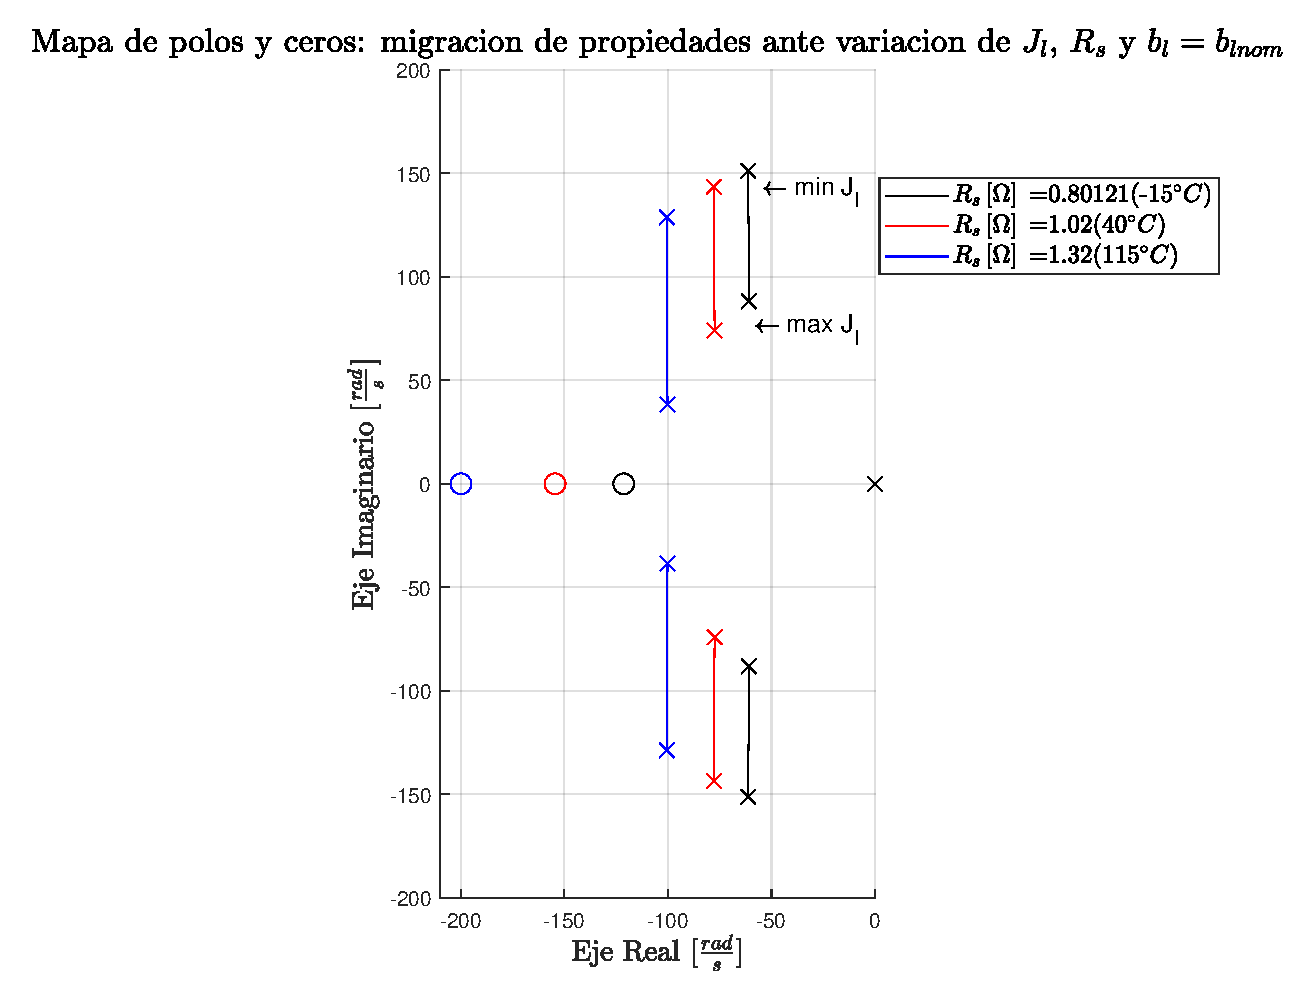
\includegraphics{33-Mapa_de_polos.pdf}}
	\end{adjustbox}
	\caption{Mapa de polos completo del sistema ante variación de $J_l$ y $R_s$ con $b_l = b_{lnom}$.}
	\label{mapa de polos b_l nominal}
\end{figure}

\begin{figure}[H]
	\centering
	\begin{adjustbox}{scale=0.5,max width=\columnwidth}
		\framebox{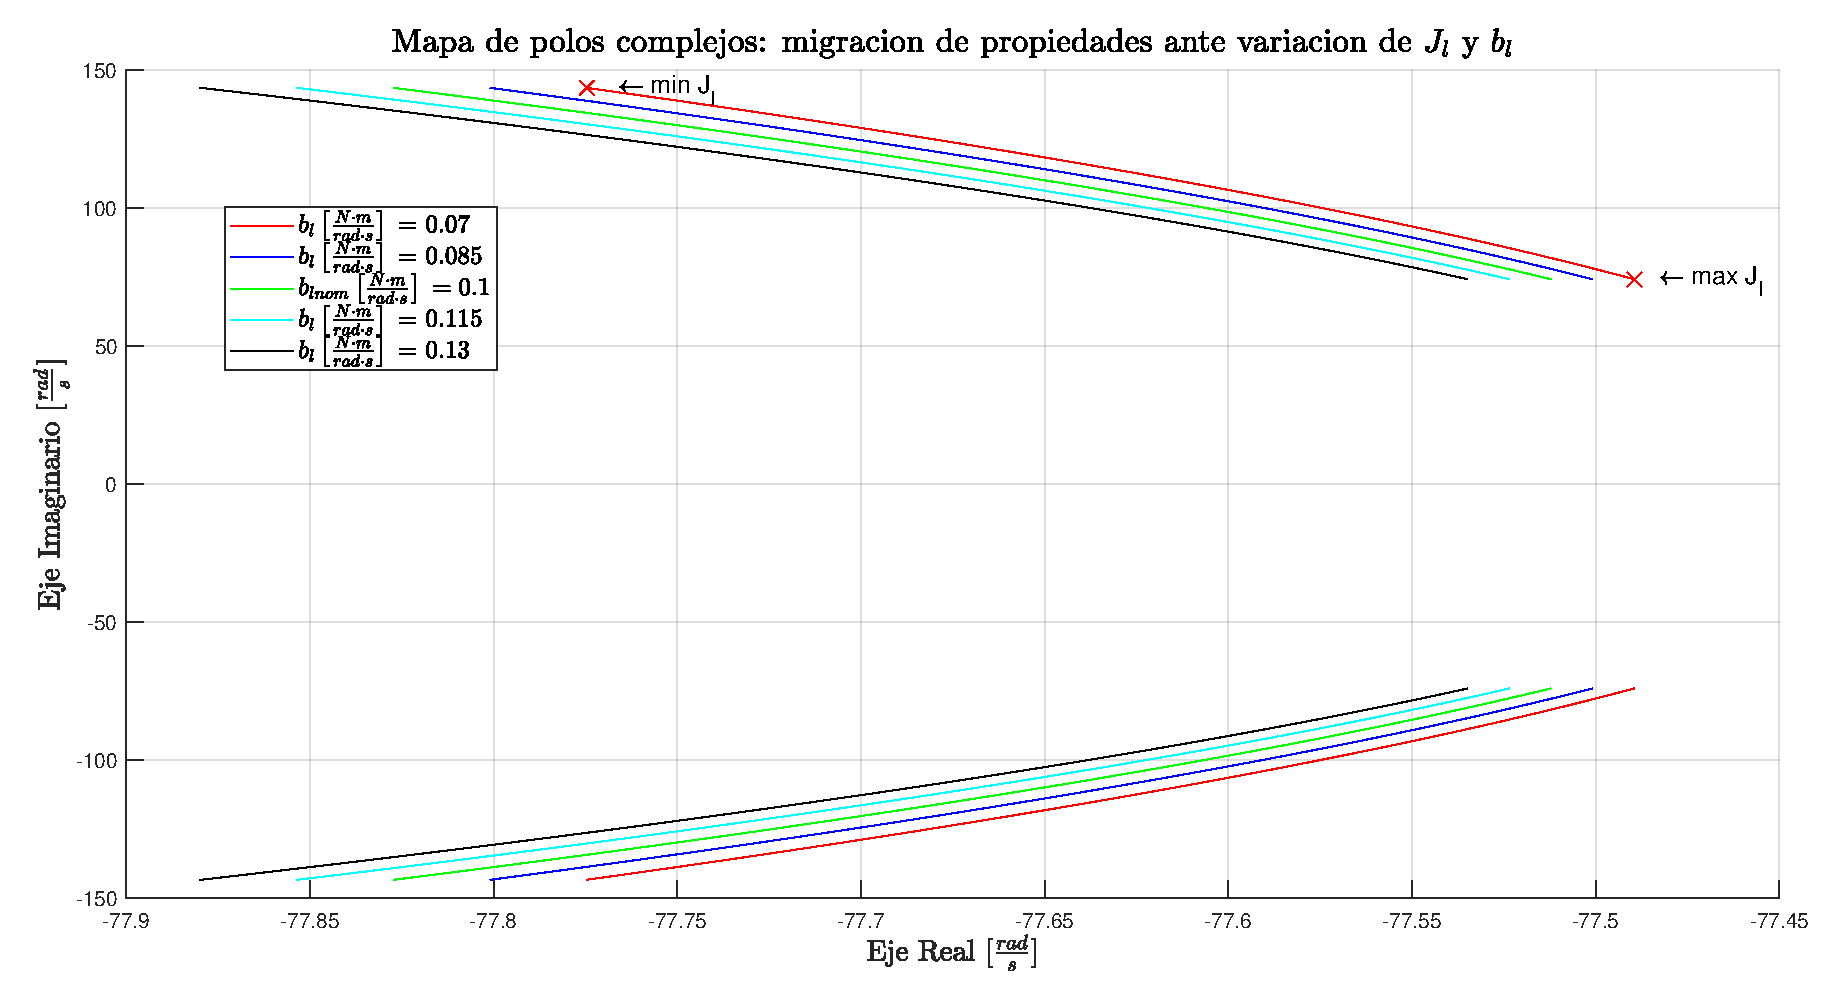
\includegraphics{34-Mapa_de_polos_complejos_migracion.pdf}}
	\end{adjustbox}
	\caption{Mapa de polos complejos del sistema ante variación de parametros de la carga ($R_s$ a $40^\circ C$).}
	\label{mapa de polos complejos}
\end{figure}

A continuación se trazaron las curvas que presentan la variación
de $\omega_n$ (\cref{variacion de omega_n}) y de $\zeta$ (\cref{variacion de zita}). Cómo se anticipó,
la variación de $b_l$ no tiene efecto apreciable en el cambio de $\omega_n$ y se presentan prácticamente superpuestas
las curvas de $\omega_n$ respecto a $J_l$ para cada $b_l$ y de manera similar ocurre para la variación de $\zeta$.
Es por eso que, en lugar de presentar las curvas para todo el rango de variación de $b_l$, lo que no aportaría claridad
a la explicación al presentarse las gráficas superpuestas, lo que se hace es tomar $b_l = b_{lnom}$ y graficar la variación
solo respecto a $R_s$ y $J_l$. Se puede observar que aunque $R_s$ tampoco produce demasiado efecto en $\omega_n$ si lo hace en $\zeta$.

\begin{figure}[H]
	\centering
	\begin{adjustbox}{scale=0.5,max width=\columnwidth}
		\framebox{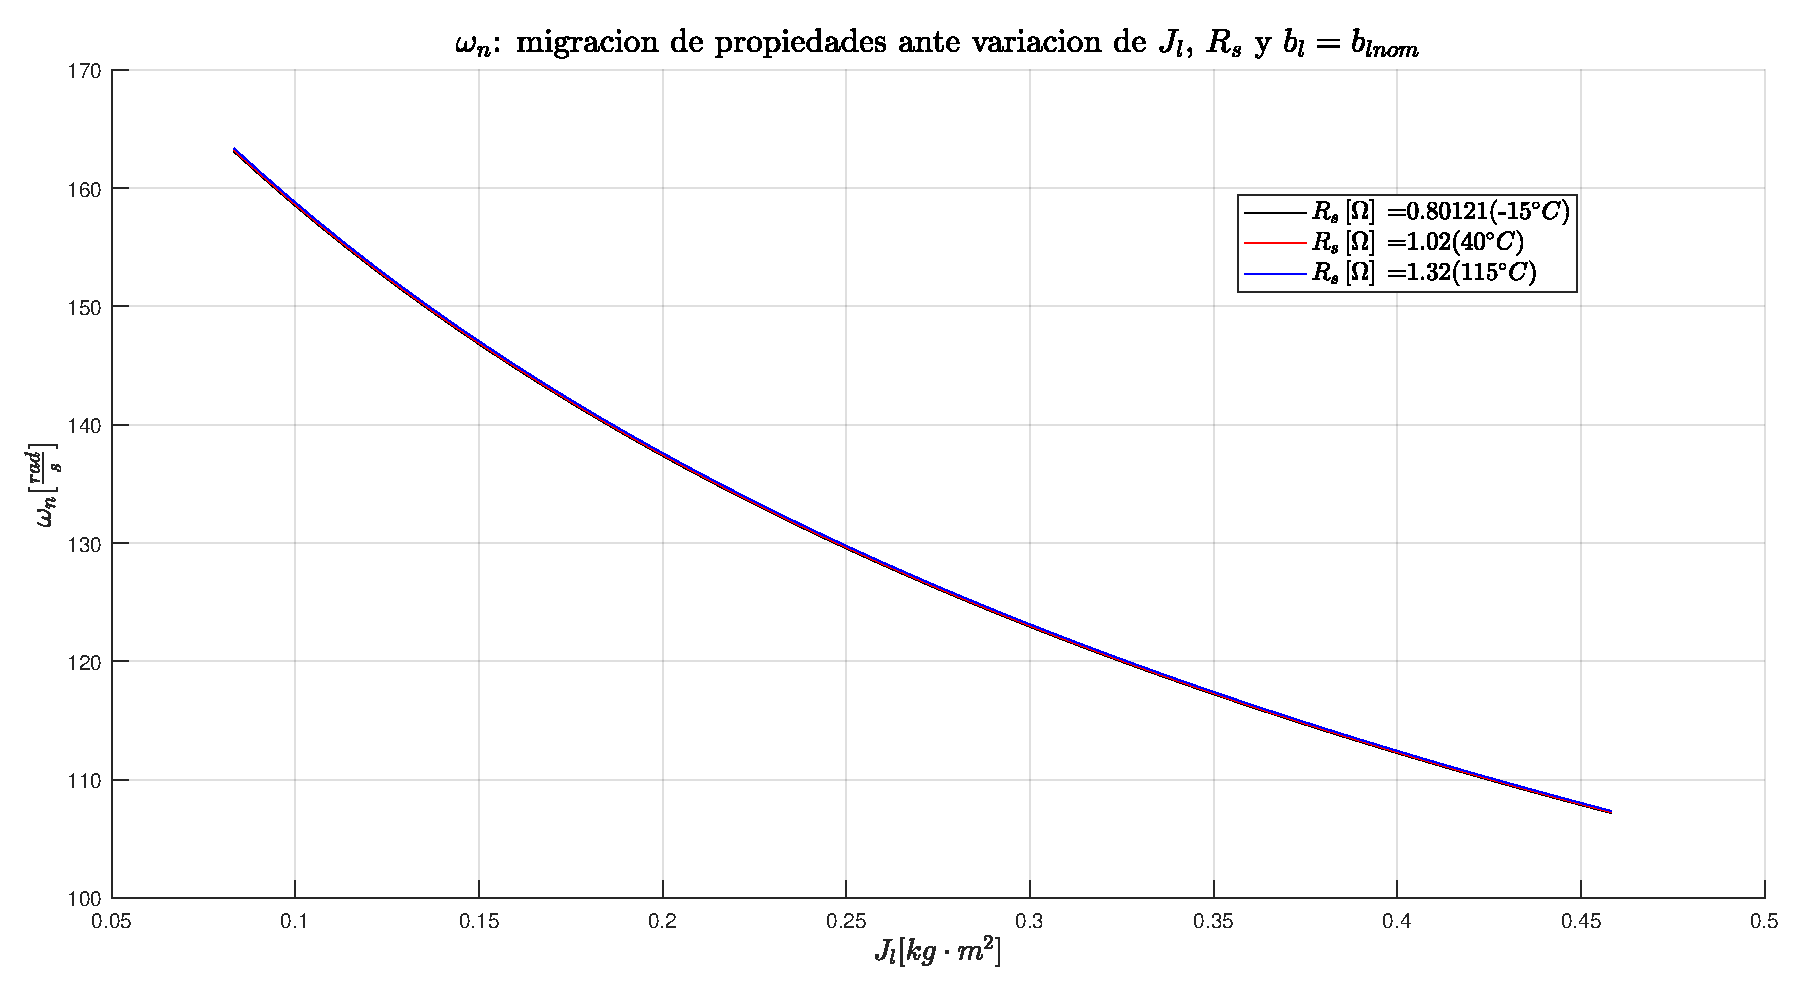
\includegraphics{35-Frecuencia_natural_migracion.pdf}}
	\end{adjustbox}
	\caption{Variación de la frecuencia natural (ancho de banda del sistema) $\omega_n$ ante variación de los parámetros de la carga y de $R_s$.}
	\label{variacion de omega_n}
\end{figure}

\begin{figure}[H]
	\centering
	\begin{adjustbox}{scale=0.5,max width=\columnwidth}
		\framebox{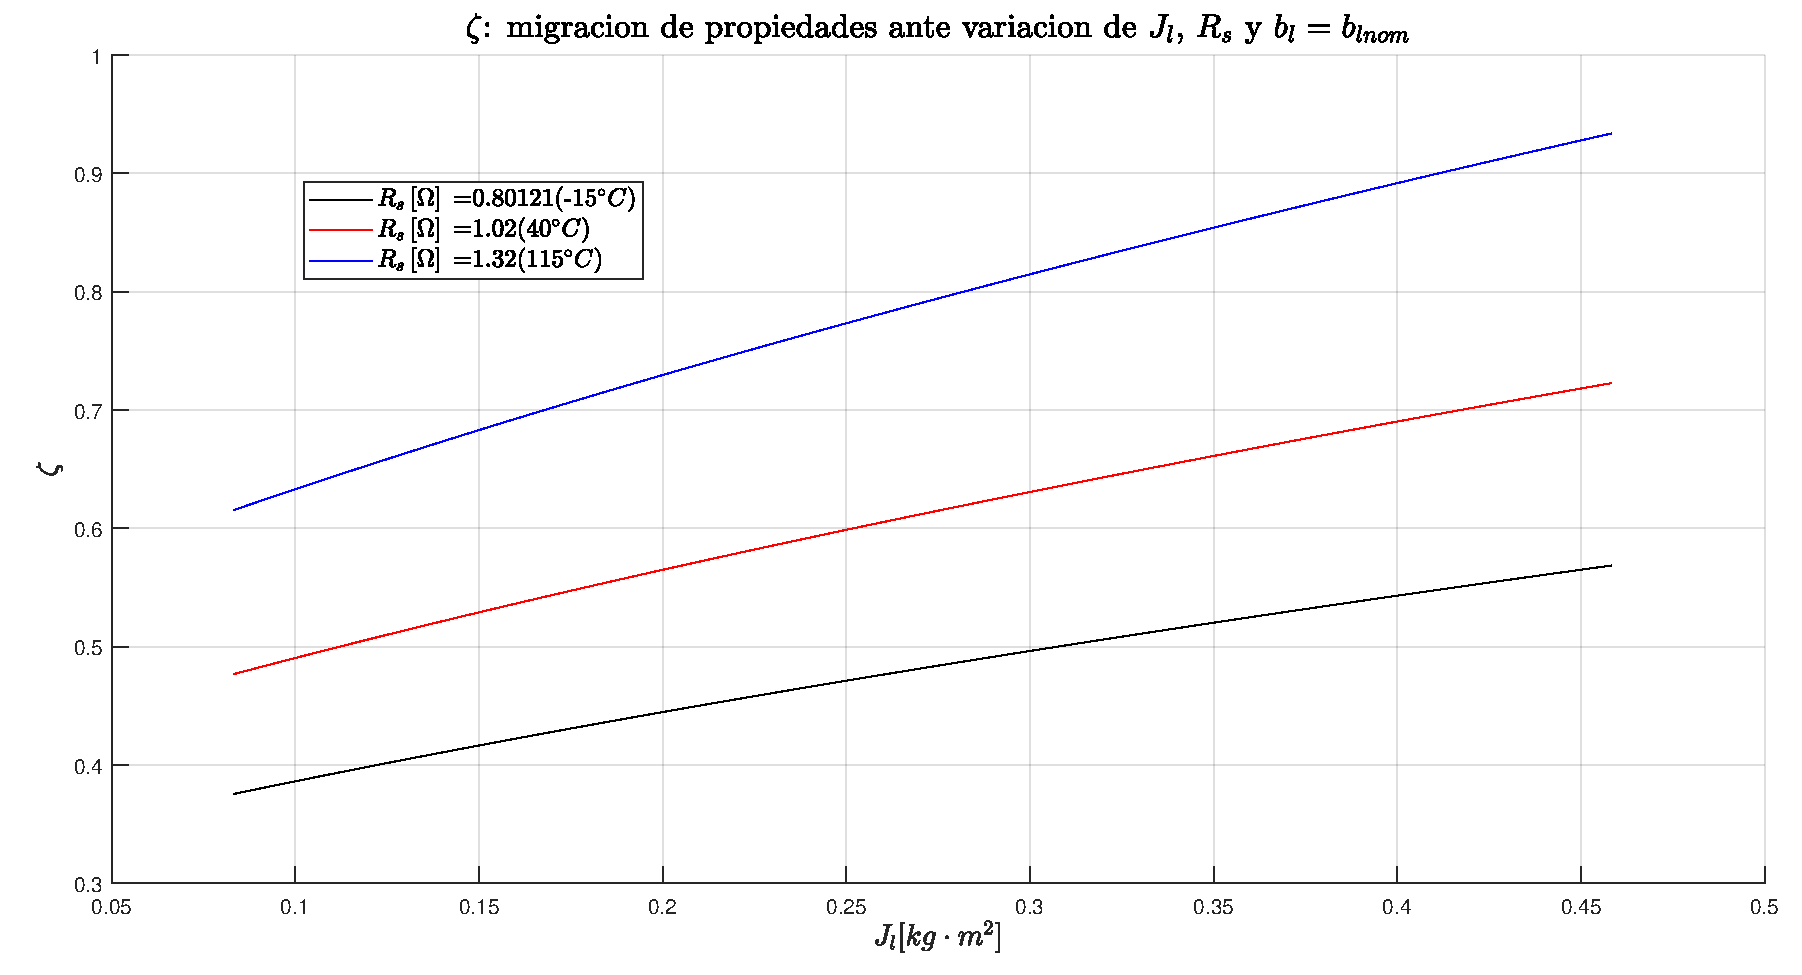
\includegraphics{36-Zita_migracion.pdf}}
	\end{adjustbox}
	\caption{Variación de la relación de amortiguamiento crítico $\zeta$ ante variación de los parámetros de la carga y de $R_s$.}
	\label{variacion de zita}
\end{figure}

\paragraph{\textbf{Estabilidad parcial y completa, y dinámica de los ceros}}
Cómo se pudo observar en el mapa de polos y ceros (\cref{mapa de polos b_l nominal}),  ante la variación de los parámetros de la carga
y de la temperatura de equilibrio térmico, los polos siempre se encuentran
en el semiplano izquierdo del plano complejo (a excepción del polo en el origen) y esta es condición suficiente para
garantizar que el \textbf{sistema es estable}. Por otro lado, el polo en el origen no introduce una inestabilidad real, 
en cambio, está asociado a un crecimiento sin cota del pseudo-estado $\theta_m(t)$ al no considerarse ahora, explícitamente,
la rectificación de la variable angular de la articulación al rango  $[0;2\pi] rad$; o a una posición angular final constante no nula
luego de los transitorios en régimen no forzado.

Para el análisis de la dinámica de los ceros, primero %aca deberíamos hacer un \cite{canal del tipo de control}
expresamos la \cref{funcion de transferencia desde T_l}
como:

\begin{equation}
    \begin{cases}
        z &= -R_s/L_q\\
        G_1(s) &= -\frac{-\frac{L_q}{r}z}{J_{eq} L_{q} s^3 +\left( J_{eq} R_{s} + L_{q} b_{eq} \right)s^2 + \left( R_{s} b_{eq} + \dfrac{3}{2} {P_{p}}^2 { \lambda^{'r}_m}^2\right) s}\\
	    G_{T_l}(s) &= G_1(s)\left( 1 - \frac{s}{z}\right)
    \end{cases}
	\label{funcion de transferencia desde T_l simplificada}
\end{equation}

En la \cref{funcion de transferencia desde T_l simplificada}, $G_1(s)$ da la respuesta a una entrada $T_l(s)$
y la respuesta total a través de $G_{T_l}(s)$ se obtiene sumando a la obtenida de $G_1(s)$ su derivada
ponderada por un factor $\rho = -1/z$. En tanto mayor sea el valor de $\rho$ (tanto más cercano al eje imaginario se encuentra $z$)
mayor será la ponderación de la derivada. Ante una entrada tipo escalón,
este cero amplifica el sobrepico en el transitorio en el punto de inflexión de la respuesta a la salida de 
$G_1(s)$. Para representar este fenómeno, se simuló el sistema bajo las condiciones indicadas en la \cref{condiciones simulacion dinamica de ceros},
primero con los parámetros nominales del sistema y luego exagerando
el efecto del cero llevándolo hacia el eje imaginario. Los resultados se muestran en la \cref{dinámica de cero nominal} y en la \cref{dinámica de cero exagerada} respectivamente.
Cómo se puede observar en las mismas, presentamos la evolución en el tiempo de $\omega_m(t)$ en lugar de $\theta_m(t)$.
Hacemos esto, dado que, al ser el último un pseudo-estado, en estado permanente crece sin cota a diferencia de $\omega_m(t)$ que sí adopta un valor permanente constante ante la perturbación de tipo escalón, y de la misma
manera permite reflejar el efecto del cero en la dinámica a lazo abierto.


\begin{equation}
    \begin{cases}
        \mathbf{x}(0) &= \mathbf{0}\\
        v^r_{qs}(t) &\equiv 0\\
        T_l(t) &= 0 \rightarrow  \left(T_{lmax} = 6.28 \, N \cdot m\,; t = 1\,s\right)\\
        \left(1\right)\rightarrow z &= z_{nom} = -154.54\left[\frac{rad}{s}\right]\left(\cref{cero del sistema LTI}\right)\\
	    \left(2\right)\rightarrow z &= -60\,\frac{rad}{s}
    \end{cases}
	\label{condiciones simulacion dinamica de ceros}
\end{equation}
 
\begin{figure}[H]
	\centering
	\begin{adjustbox}{max width=\columnwidth}
		\framebox{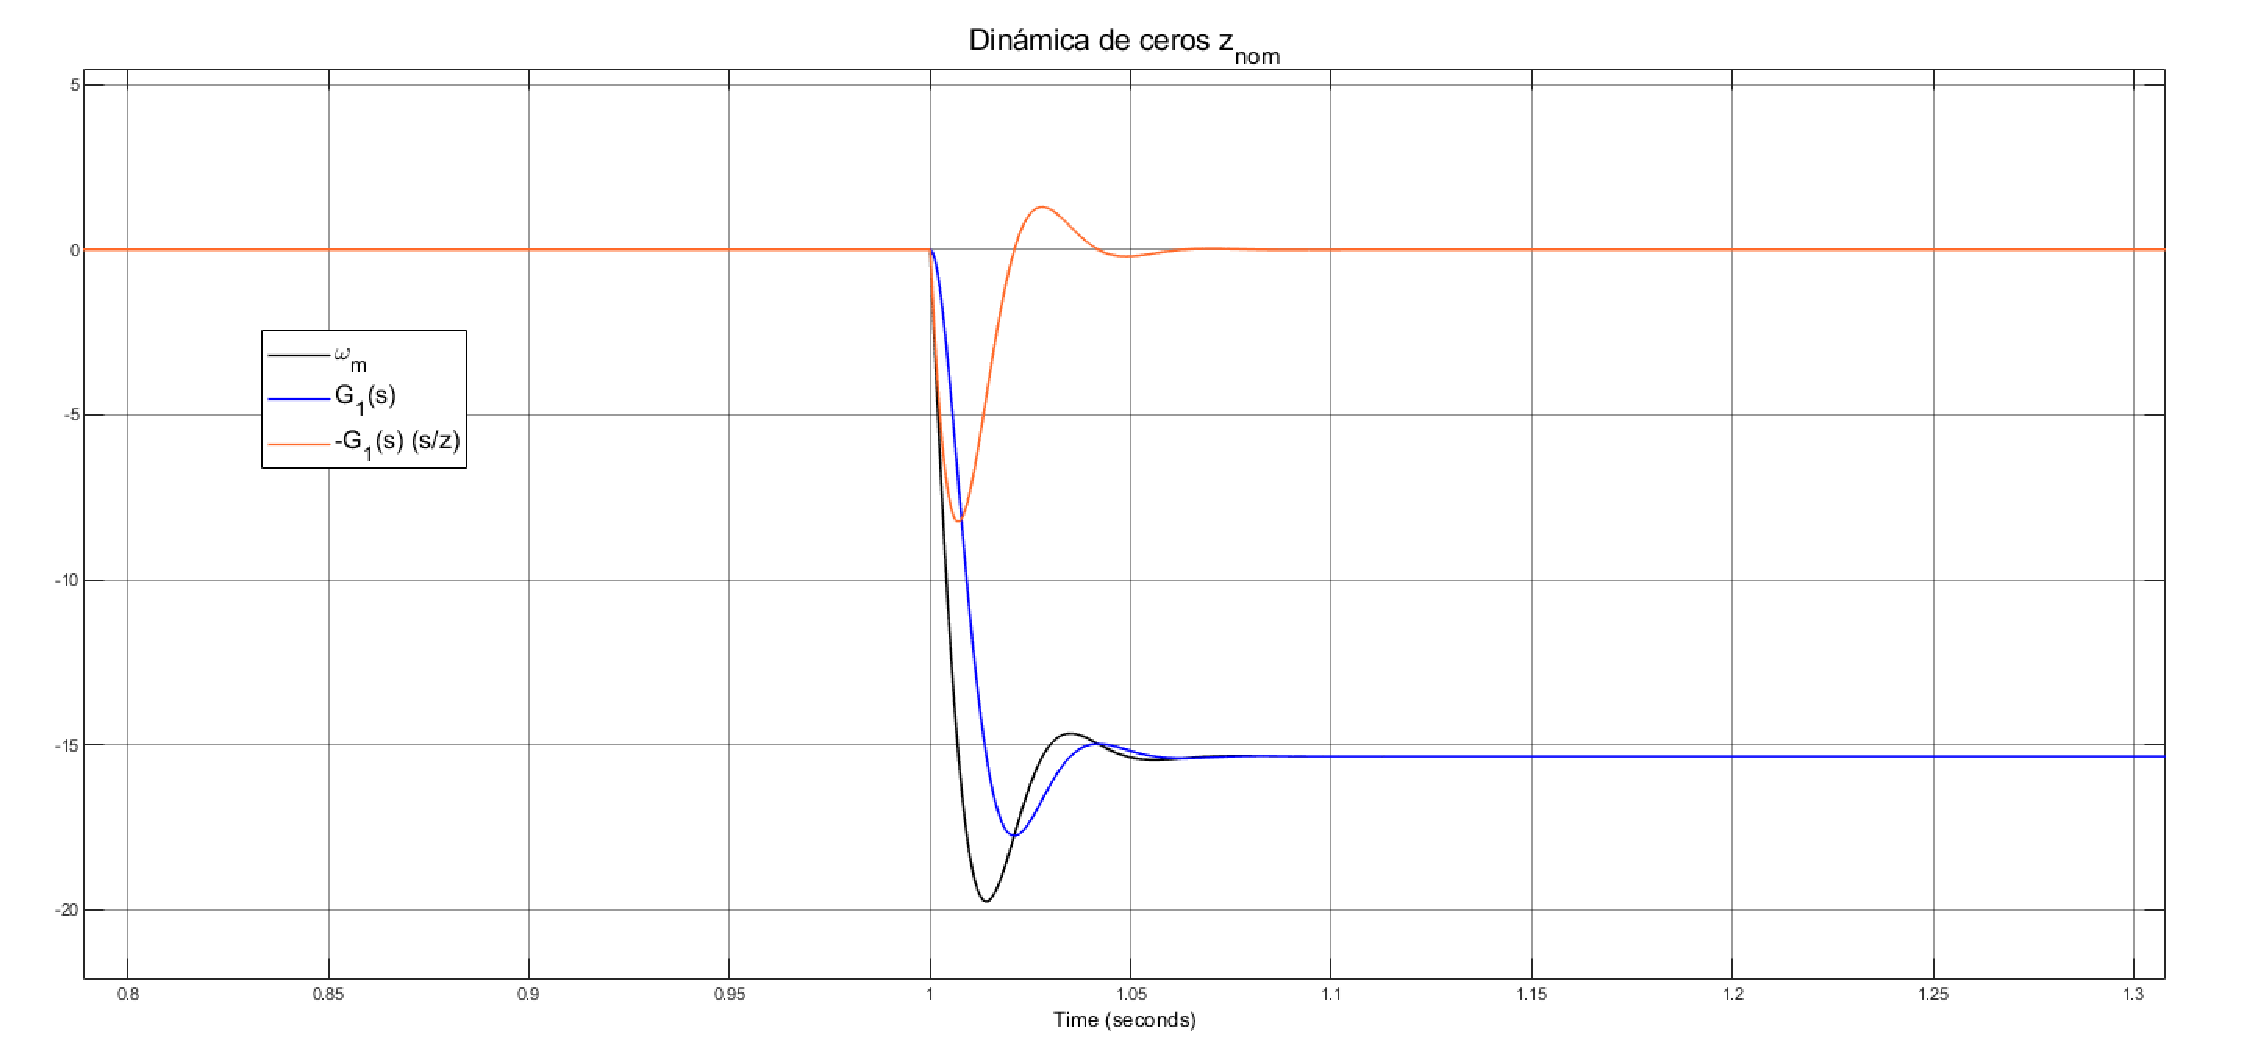
\includegraphics{37-Dinamica_de_los_ceros_1.pdf}}
	\end{adjustbox}
	\caption{Dinámica del cero de $G_{T_l}(s)$ para $z_{nom}$.}
	\label{dinámica de cero nominal}
\end{figure}

\begin{figure}[H]
	\centering
	\begin{adjustbox}{max width=\columnwidth}
		\framebox{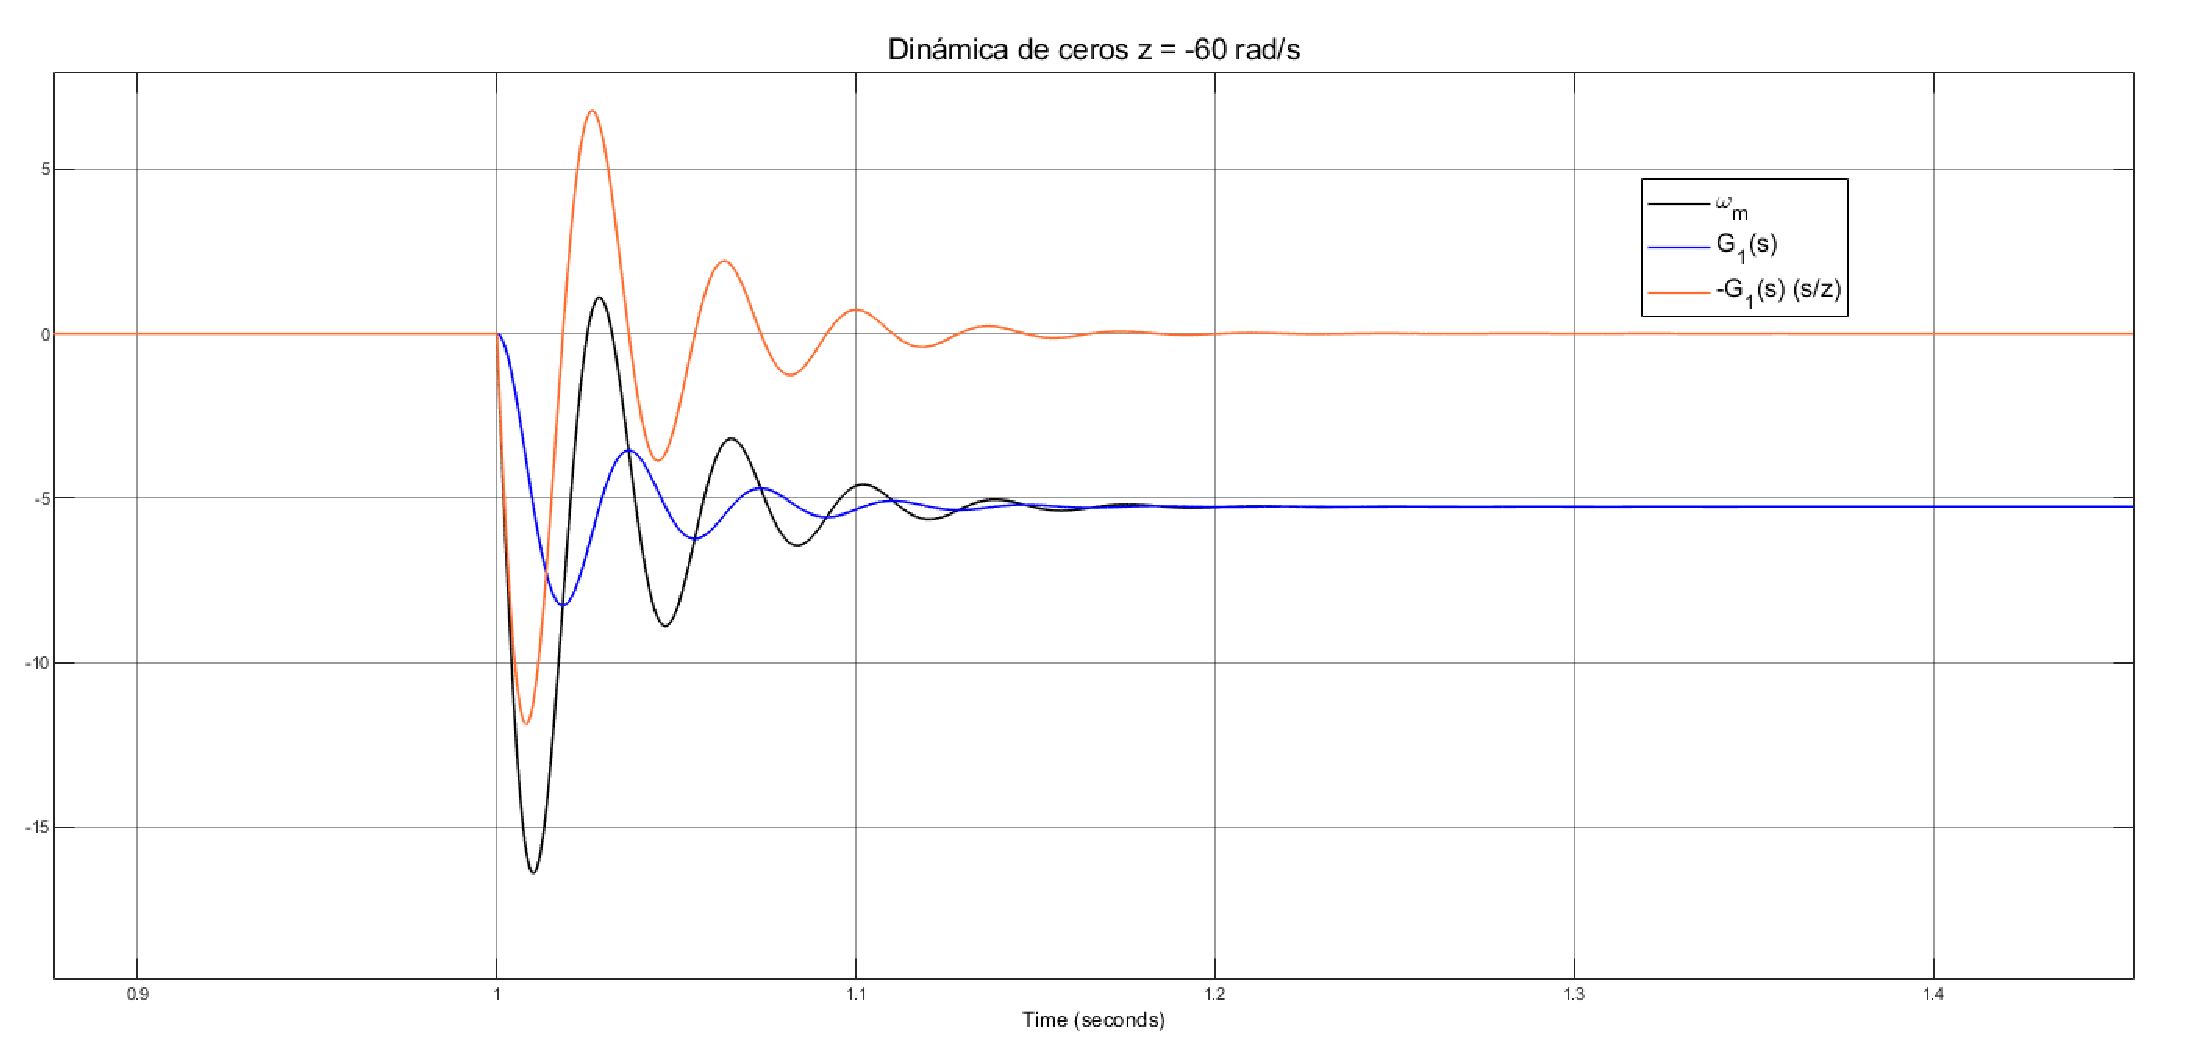
\includegraphics{38-Dinamica_de_los_ceros_2.pdf}}
	\end{adjustbox}
	\caption{Dinámica del cero de $G_{T_l}(s)$ para $z$ trasladado hacia el eje imaginario.}
	\label{dinámica de cero exagerada}
\end{figure}

\subsubsection{\textbf{Análisis de observabilidad completa de estado para el modelo LTI equivalente aumentado desde salida medida $\mathbf{\theta_m(t)}$}}

Para evaluar la observabilidad desde la salida medida, se determinó la matriz de observabilidad, para luego calcular su rango y compararlo con el orden del sistema.

\begin{equation}
	O=
	\begin{bmatrix}
		C \\ 
		CA\\
		...\\
		CA^{n-1}  
	\end{bmatrix}
	\label{Matriz de observabilida generica}
\end{equation}

Para nuestro caso, recordando las matrices A y C en la \cref{ecuacion matricial con ids=0}, la matriz de observabilidad quedó de la siguiente manera:
\begin{equation}
	O=
	\begin{bmatrix}
		1 & 0 & 0 \\ 
		0 & 1 & 0\\
		 0 & -\frac{b_{eq}}{J_{eq}} & \frac{3 P_p \lambda^{'r}_m}{2 J_{eq}}  
	\end{bmatrix}
	\label{Matriz de observabilida del LTI}
\end{equation}

Al calcular el determinante de esta matriz(\cref{determinante de Matriz de observabilida del LTI}), se pudo ver que es distinto de cero, por lo que el rango de O es 3, que es igual al orden del sistema. Entonces, se concluye que el sistema LTI aumentado simplificado es completamente observable desde la posición.

\begin{equation}
	det(O)= \frac{3 P_p \lambda^{'r}_m}{2 J_{eq}}
	\label{determinante de Matriz de observabilida del LTI}
\end{equation}

Sin embargo, se debe aclarar que el sistema LTI aumentado con sistemas autónomos desacoplados, es parcialmente observable, ya que los estados ${i}^r_{ds}(t) $ y ${T}^\circ_s(t)$ no pueden ser observados desde la posición.

Se propuso tomar como salida a la velocidad ${\omega}_m(t)$ y analizar la observabilidad desde ella. En este caso la matriz de salida es:
\begin{equation}
	C=
	\begin{bmatrix}
		0 & 1 & 0  
	\end{bmatrix}
	\label{Matriz C con velocidad como salida}
\end{equation}

La matriz de observabilidad se muestra en la \cref{Matriz de observabilidad desde velocidad del LTI}.
Al calcular el determinante de esta matriz, el resultado fue 0, por lo tanto el rango es menor a 3 y el sistema no es completamente observable desde la velocidad.

Esto ocurre ya que, al conocer la velocidad, no podemos determinar la posición instantánea sin conocer su valor inicial.

\begin{equation}
	O=
	\begin{bmatrix}
		0 & 1 & 0 \\ 
		0 & -\frac{b_{eq}}{J_{eq}} &\frac{3 P_p \lambda^{'r}_m}{2 J_{eq}}\\
		0 & \frac{2 L_q {b_{eq}}^2 - 3 J_{eq} {P_p}^2 {\lambda^{'r}_m}^2} {2 {J_{eq}}^2 L_q} & -\frac{3 P_p \lambda^{'r}_m \left(L_q b_{eq} + J_{eq} R_s \right)}{2 {J_{eq}}^2 L_q}  
	\end{bmatrix}
	\label{Matriz de observabilidad desde velocidad del LTI}
\end{equation}

\subsubsection{\textbf{Análisis de controlabilidad completa de estado para el modelo LTI equivalente aumentado desde entrada manipulada $\mathbf{v^r_{qs}(t)}$, sin considerar la perturbación de la carga mecánica}}
Para evaluar la controlabilidad desde la entrada manipulada, se determinó la matriz de controlabilidad, para luego calcular su rango y compararlo con el orden del sistema.

\begin{equation}
	S=
	\begin{bmatrix}
		B & AB & ... & A^{n-1}B  
	\end{bmatrix}
	\label{Matriz de controlabilidad generica}
\end{equation}

Para nuestro caso, recordando las matrices A y B en la \cref{ecuacion matricial con ids=0}, la matriz de controlabilidad quedó de la siguiente manera:
\begin{equation}
	S=
	\begin{bmatrix}
		0 & 0 & \frac{3 P_p \lambda^{'r}_m}{2 J_{eq} L_q}\\ 
		0 & \frac{3 P_p \lambda^{'r}_m}{2 J_{eq} L_q} & -\frac{3 P_p \lambda^{'r}_m \left(L_q b_{eq} + J_{eq} R_s \right)}{2 {J_{eq}}^2 L_q^2}\\
		\frac{1}{L_q} & -\frac{R_s}{{L_q}^2} & \frac{2 J_{eq} {R_s}^2 - 3 L_{q} {P_p}^2 {\lambda^{'r}_m}^2} {2 J_{eq} {L_q}^3}  
	\end{bmatrix}
	\label{Matriz de controlabilidad del LTI}
\end{equation}

El determinante de esta matriz (\cref{determinante de Matriz de controlabilidad del LTI}), 
como ocurrió con la de observabilidad, se pudo ver que es distinto de cero, por lo que el rango de S es 3, igual al orden del sistema. Así, el sistema LTI aumentado simplificado es completamente controlable desde $v^r_{qs}(t)$.

\begin{equation}
	det(S)= -\frac{9 {P_p}^2 {\lambda^{'r}_m}^2}{4 {J_{eq}}^2 {{L_q}}^3}
	\label{determinante de Matriz de controlabilidad del LTI}
\end{equation}

Similar a lo que ocurrió con la observabilidad, el sistema LTI aumentado con sistemas autónomos desacoplados, es parcialmente controlable, ya que el estado ${i}^r_{ds}(t) $  no puede ser controlado desde $v^r_{qs}(t)$. Para lograrlo, deben considerarse otras entradas de control adicionales como  $v^r_{ds}(t)$, haciendo
$v^{*r}_{ds}(t) \neq 0$ en la \cref{equaciones modelo LTI eq}.


\subsubsection{\textbf{Simulación dinámica en dominio temporal}} 
Se realizó una comparación entre el modelo no lineal completo desacoplado utilizando una ley de control no lineal y el modelo linealizado equivalente aumentado. En esta comparación, se analizaron dos escenarios: uno con $i^r_{ds}(0) = \pm 0.5 \, A $  y otro con $i^r_{ds}(0) = 0 \, A $ 
\paragraph{\textbf{Respuesta del estado interno a pulso de consigna de tensión de estator en eje q}}
Primero se analizó la respuesta del estado interno $\left\lbrace \theta_m(t), \omega_{m}(t), i^r_{qd0s}(t), T^\circ_s(t)\right\rbrace $ y $v^r_{ds}(t)$ forzada a un pulso de consigna de tensión en eje q, \cref{pulso de tensión}, superpuesto con doble pulso de torque de carga, \cref{doble pulso de torque}.

\begin{equation}
	{v^r_{qs}(t)}^* = 0 \rightarrow \left({v^r_{qs}}^* = +19.596 \: V_{cc} \  en \ t_{step1}=0.1s \right) \rightarrow \left(0 \: V \  en \ t_{step4}=0.7s \right)
	\label{pulso de tensión}
\end{equation}

\begin{equation}
	T_{l}(t) = 0 \rightarrow \left(T_{lmax} = +6.28 \: Nm \ ; \ t_{step2}=0.3s \right) \rightarrow \left(-T_{lmax} = -6.28 \: Nm \ ; \ t_{step3}=0.5s \right)
	 \rightarrow \left(0 \: Nm \ ; \ t_{step5}=0.9s \right) 
	 \label{doble pulso de torque}
\end{equation}
Se adopta una temperatura ambiente de 40 °C debido a que esta fue la que se consideró al calcular la resistencias de los devanados. Las graficas de las entradas quedan entonces de la siguiente manera.


\begin{figure}[H]
	\centering
	\begin{adjustbox}{max width=\columnwidth}
		\framebox{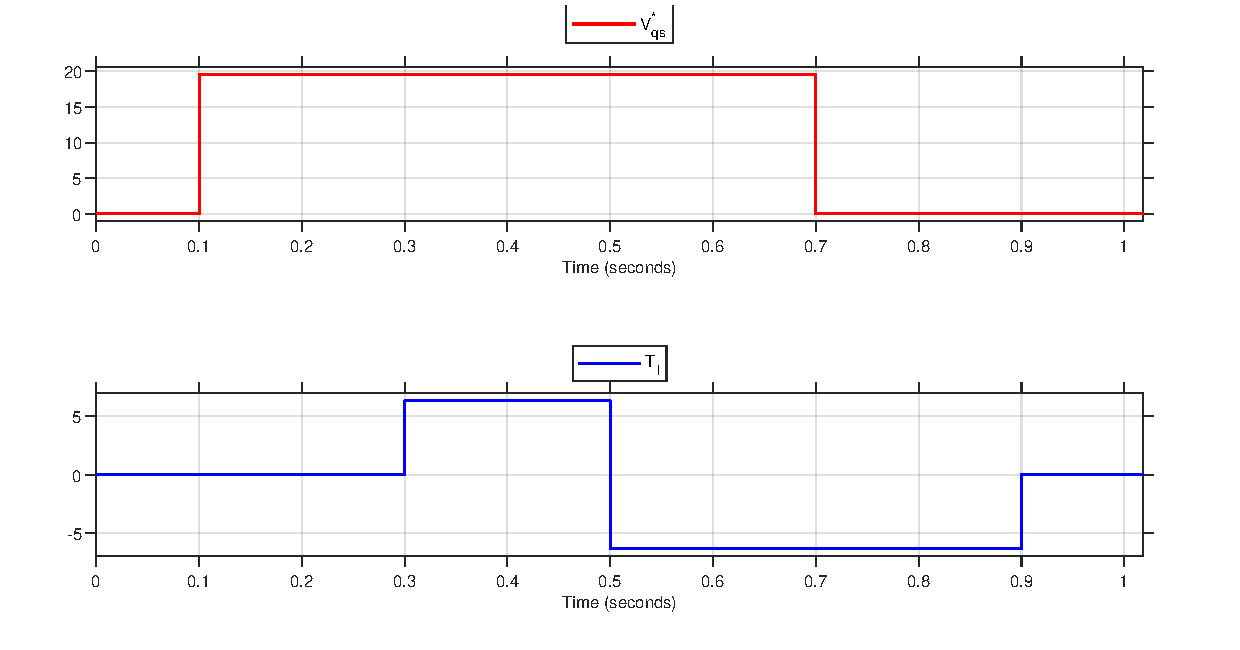
\includegraphics{39-Consignas_simulacion_5_1_6.pdf}}
	\end{adjustbox}
	\caption{Consigna de tensión y torque de perturbación}
	\label{Consigna de tensión y torque de perturbación.}
\end{figure}
Al simular el sistema con estas entradas, se obtuvieron las siguientes respuestas para la temperatura de los devanados, posición y velocidad del motor de ambos sistemas.

\begin{figure}[H]
	\centering
	\begin{adjustbox}{max width=\columnwidth}
		\framebox{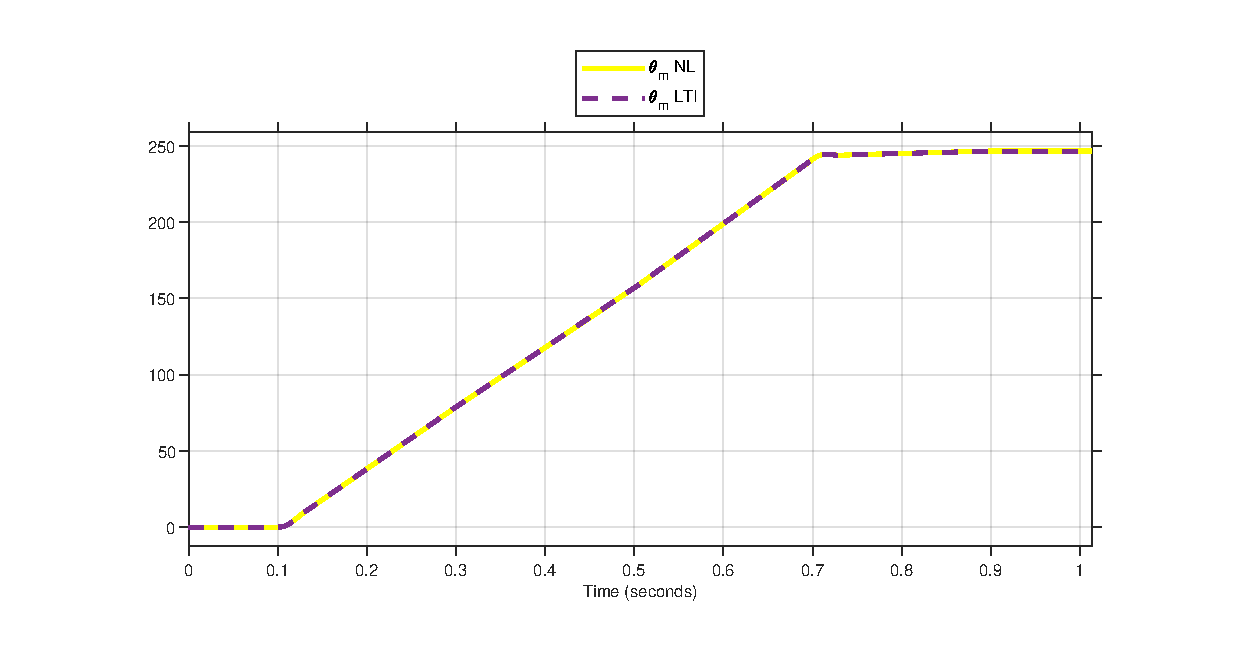
\includegraphics{40-Posiciones_simulacion_5_1_6.pdf}}
	\end{adjustbox}
	\caption{Posición motor del sistema NL realimentado y del LTI aumentado.}
	\label{Posición motor del sistema NL realimentado y del LTI aumentado}
\end{figure}
\begin{figure}[H]
	\centering
	\begin{adjustbox}{max width=\columnwidth}
		\framebox{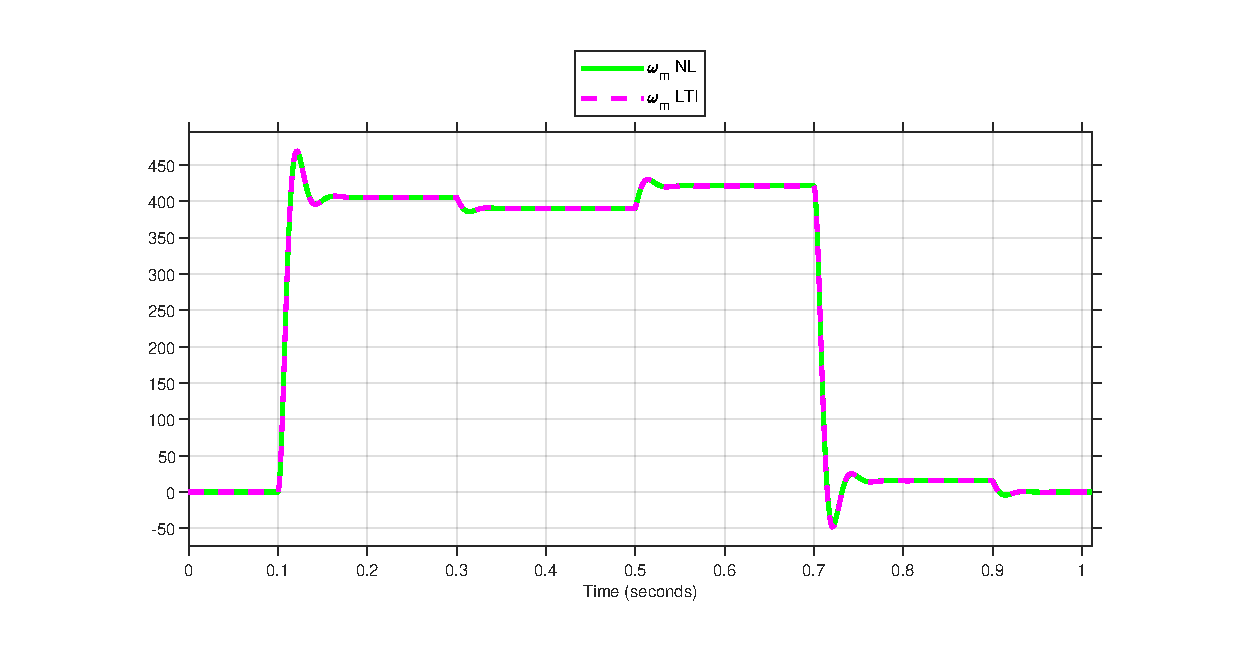
\includegraphics{41-Velocidades_simulacion_5_1_6.pdf}}
	\end{adjustbox}
	\caption{Velocidad motor del sistema NL realimentado y del LTI aumentado.}
	\label{Velocidad motor del sistema NL realimentado y del LTI aumentado}
\end{figure}
\begin{figure}[H]
	\centering
	\begin{adjustbox}{max width=\columnwidth}
		\framebox{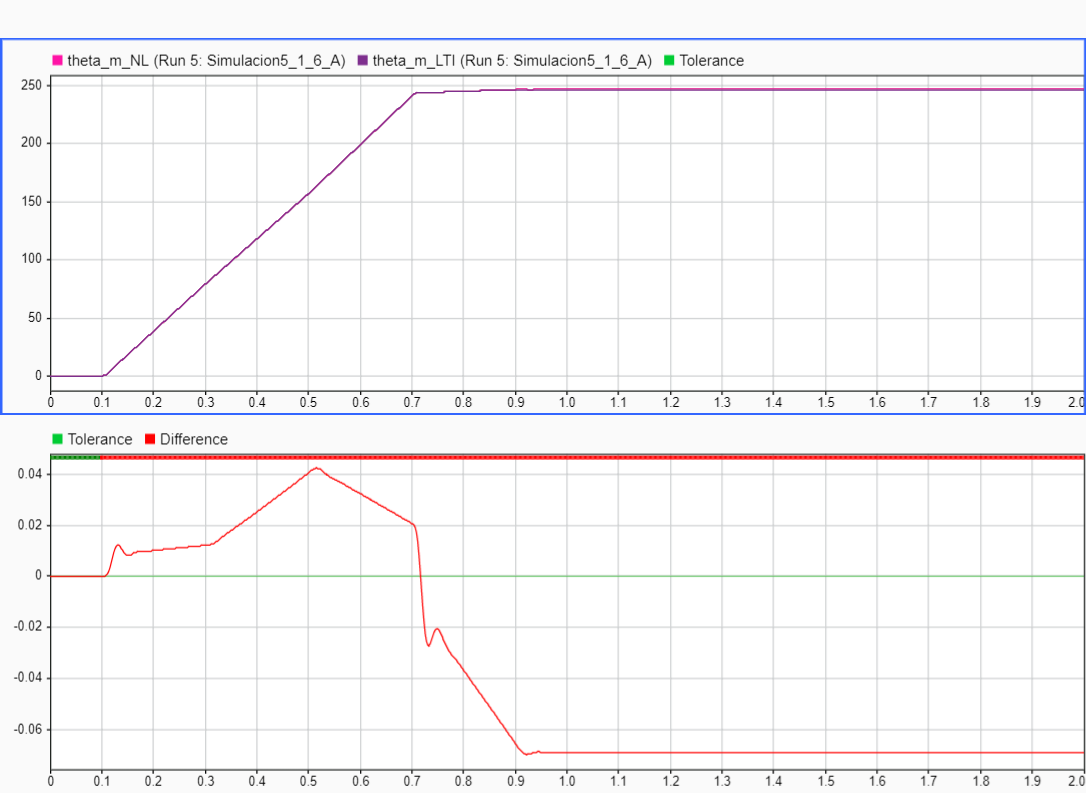
\includegraphics{42-5-Error_posicion_LTI_vs_NL}}
	\end{adjustbox}
	\caption{Diferencia entre la posición del sistema NL con la del LTI equivalente aumentado.}
	\label{Diferencia entre la posición del sistema NL con la del LTI equivalente aumentado}
\end{figure}
\begin{figure}[H]
	\centering
	\begin{adjustbox}{max width=\columnwidth}
		\framebox{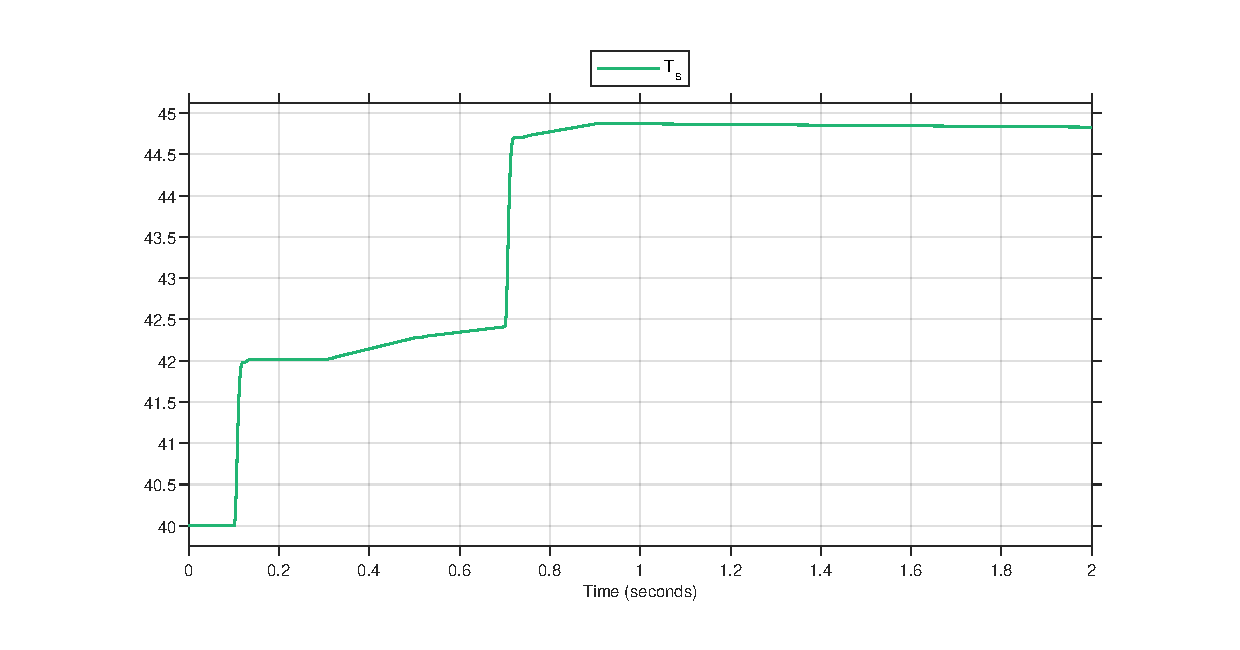
\includegraphics{42-Temperatura_simulacion_5_1_6.pdf}}
	\end{adjustbox}
	\caption{Temperatura.}
	\label{Temperatura}
\end{figure}
Se observa que los dos modelos se comportan prácticamente de la misma manera ya que la temperatura aumenta poco. Esto evidencia la eficacia de las compensaciones realizadas en el modelo NL realimentado.
Luego se graficaron las tensiones y corrientes obtenidas en coordenadas abc y qd0.
\begin{figure}[H]
	\centering
	\begin{adjustbox}{max width=\columnwidth}
		\framebox{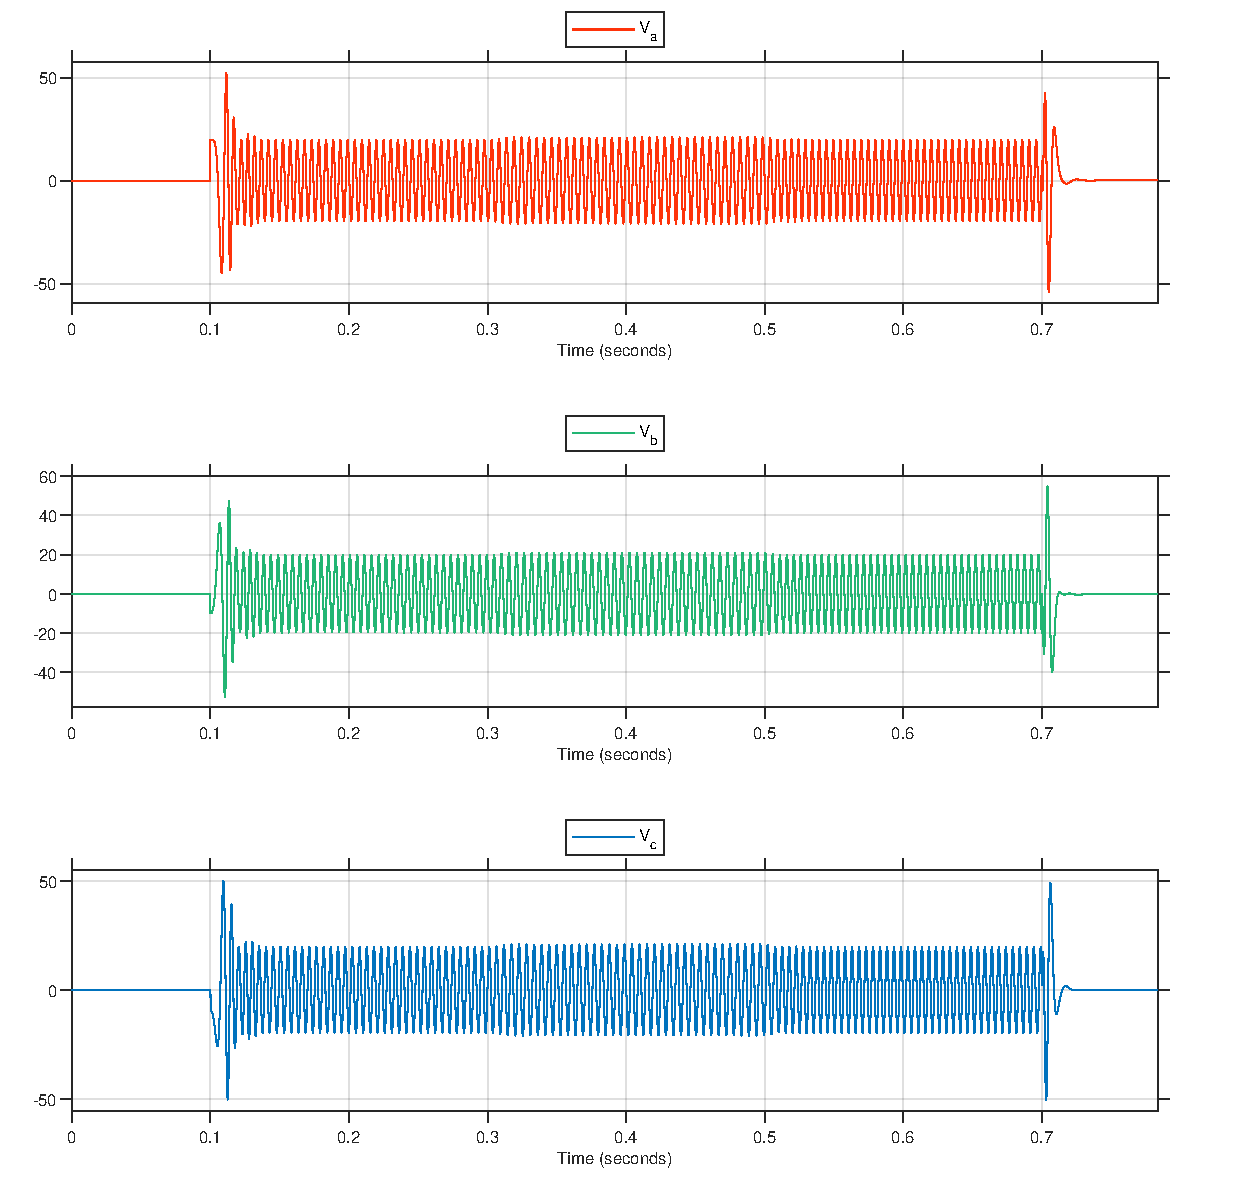
\includegraphics{43-Tensiones_abc_simulacion_5_1_6.pdf}}
	\end{adjustbox}
	\caption{Tensiones abc.}
	\label{Tensiones abc}
\end{figure}

\begin{figure}[H]
	\centering
	\begin{adjustbox}{max width=\columnwidth}
		\framebox{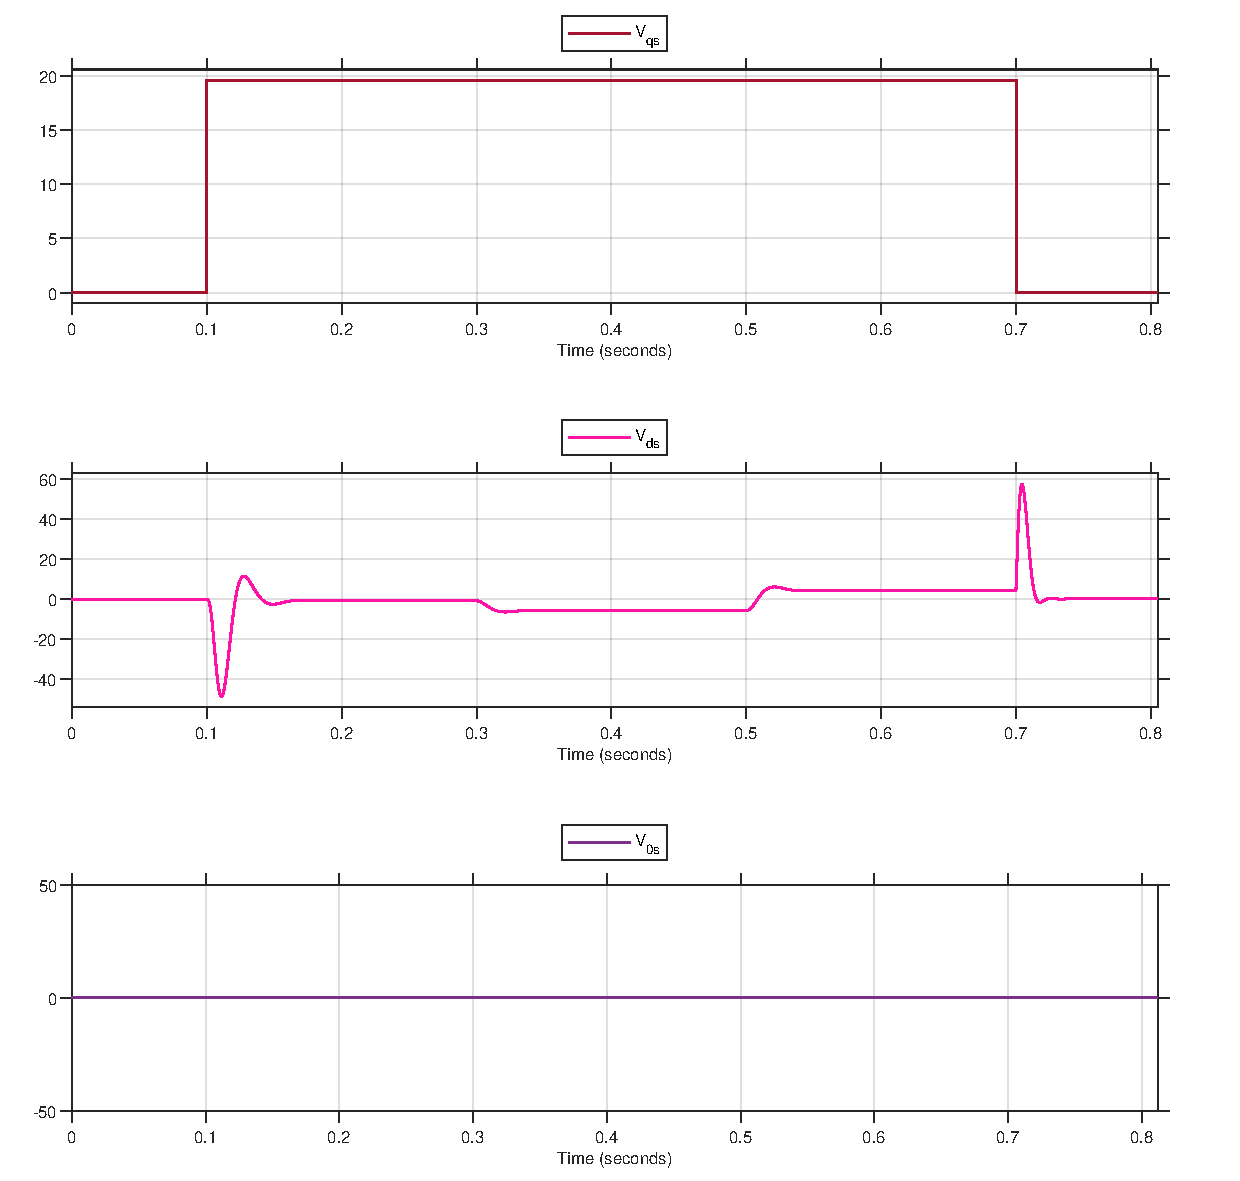
\includegraphics{44-Tensiones_qd0_simulacion_5_1_6.pdf}}
	\end{adjustbox}
	\caption{Tensiones qd0.}
	\label{Tensiones qd0}
\end{figure}

\begin{figure}[H]
	\centering
	\begin{adjustbox}{max width=\columnwidth}
		\framebox{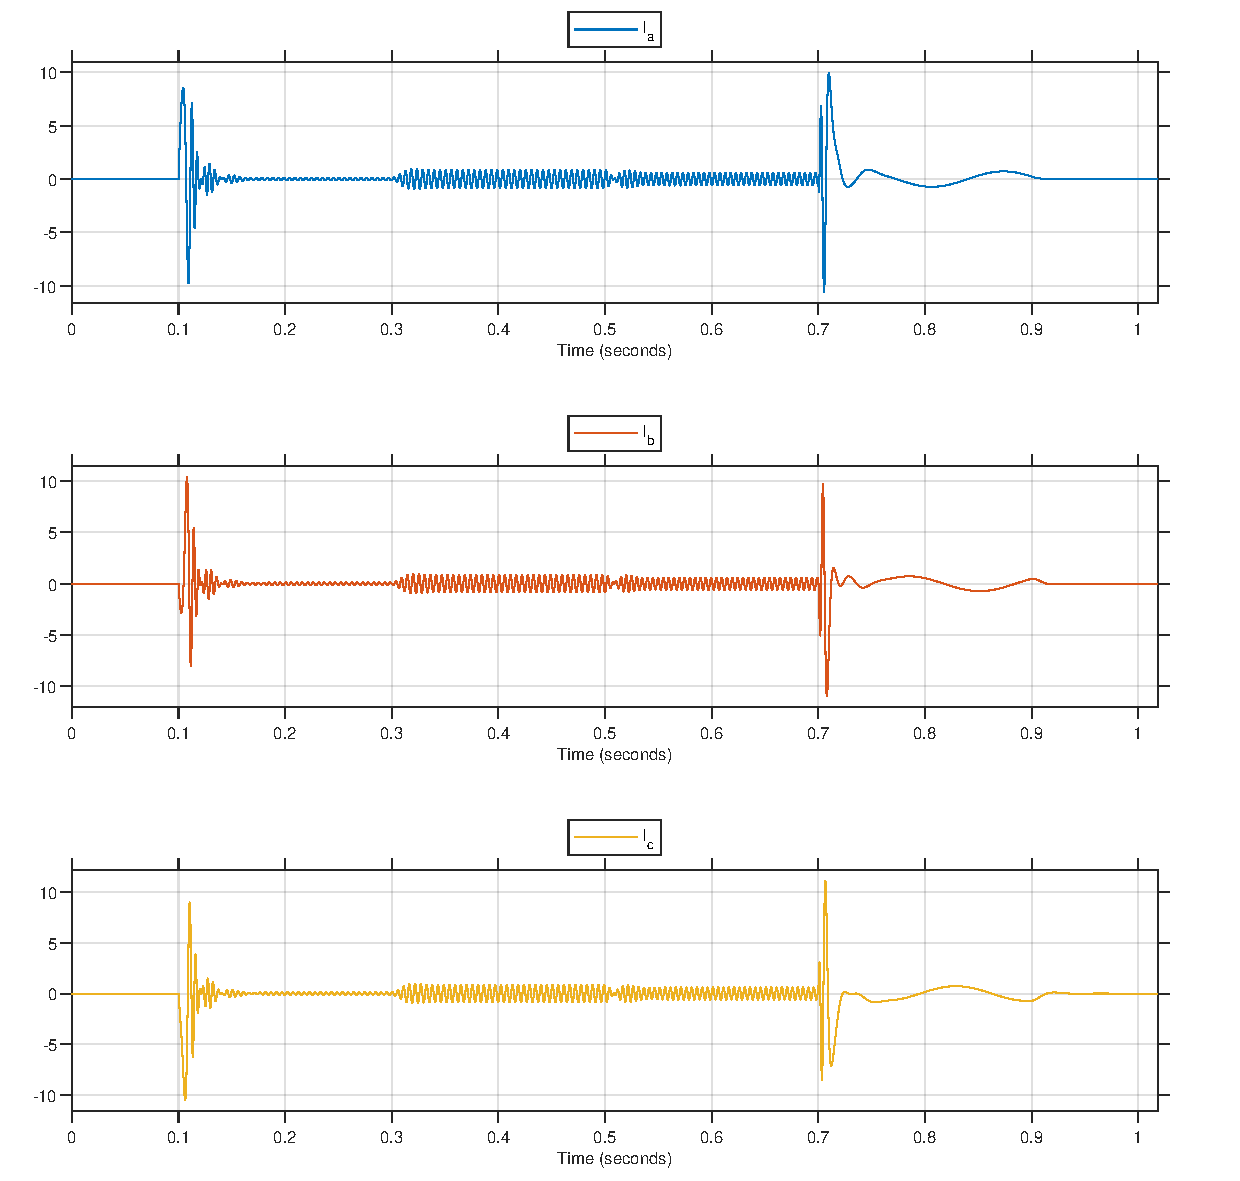
\includegraphics{45-Corrientes_abc_simulacion_5_1_6.pdf}}
	\end{adjustbox}
	\caption{Corrientes abc.}
	\label{Corrientes abc}
\end{figure}

\begin{figure}[H]
	\centering
	\begin{adjustbox}{max width=\columnwidth}
		\framebox{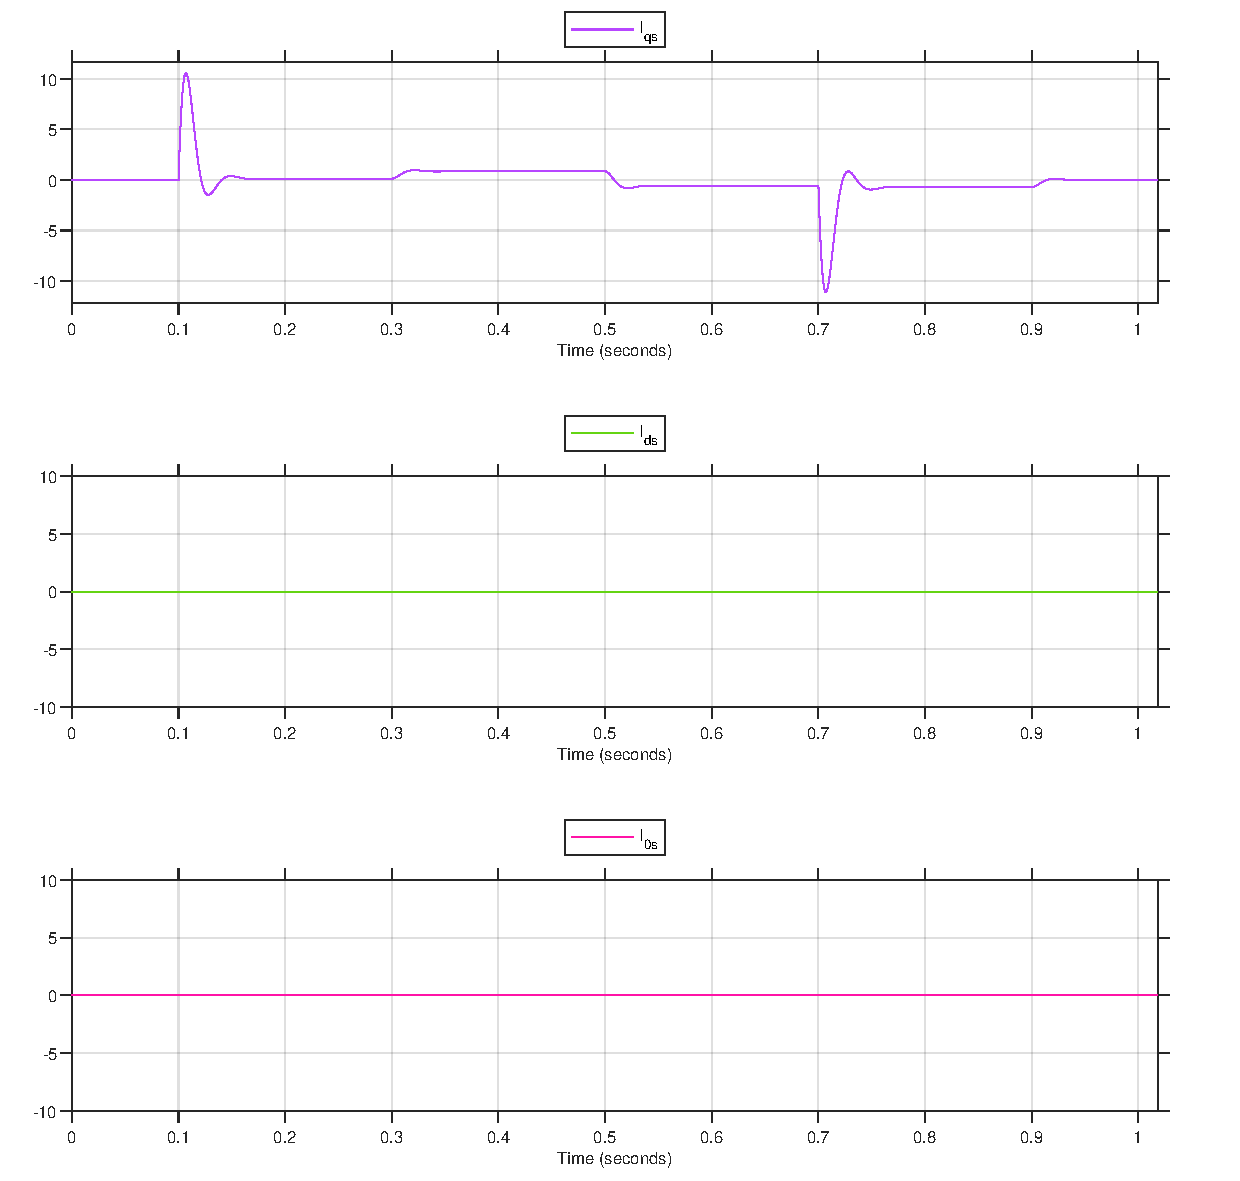
\includegraphics{46-Corrientes_qd0_simulacion_5_1_6.pdf}}
	\end{adjustbox}
	\caption{Corrientes qd0.}
	\label{Corrientes qd0}
\end{figure}
Se observa que los valores de estas tensiones y corrientes superan los límites que soportaría el motor. Más adelante se verá como mejorar estas respuestas.

Para analizar mejor el funcionamiento de la máquina eléctrica se graficó el torque electromagnético vs la velocidad del motor. 

\begin{figure}[H]
	\centering
	\begin{adjustbox}{max width=\columnwidth}
		\framebox{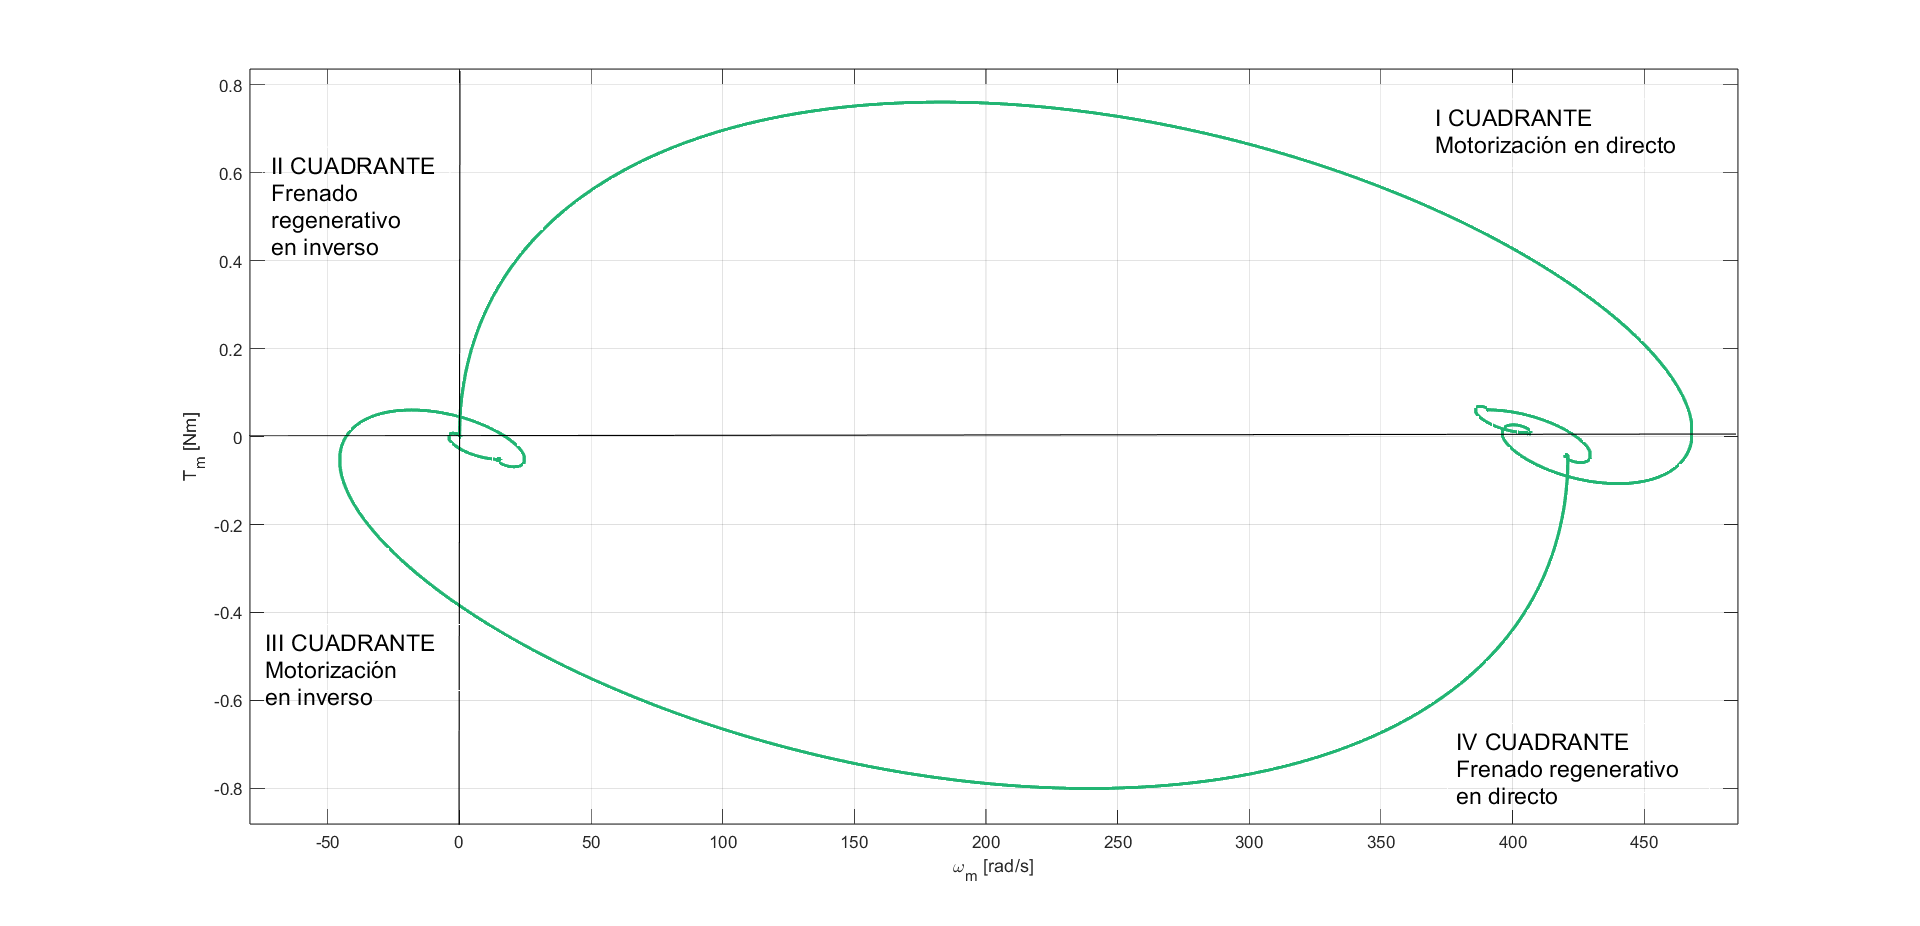
\includegraphics{47-tm_vs_vel}}
	\end{adjustbox}
	\caption{Torque electromagnético vs Velocidad del motor.}
	\label{Torque electromagnético vs Velocidad del motor}
\end{figure}
\begin{figure}[H]
	\centering
	\begin{adjustbox}{max width=\columnwidth}
		\framebox{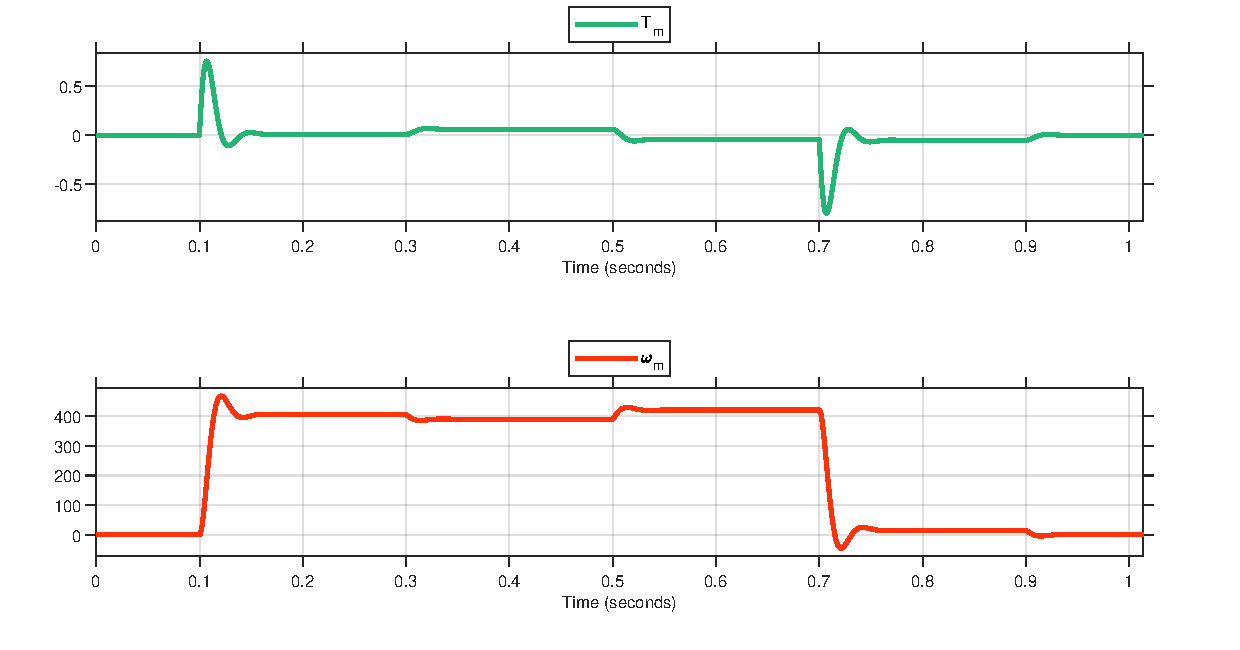
\includegraphics{48-Tm_vs_vel_m_simulacion_5_1_6}}
	\end{adjustbox}
	\caption{Torque electromagnético y Velocidad del motor.}
	\label{Torque electromagnético y Velocidad del motor}
\end{figure}
En estas graficas se observa que la máquina se comporta como motor en unos instantes y en otros como generador haciendo uso del frenado regenerativo.

\paragraph{\textbf{Determinación de las características de la respuesta}}
Para evaluar el comportamiento del sistema, se determinaron las características de respuesta de la velocidad del motor y la corriente ante escalones de consigna y torque, específicamente: tiempo de crecimiento, tiempo de establecimiento, sobrepico y valor final de establecimiento. Estos datos se obtuvieron utilizando la función ``stepinfo'' de MATLAB\textsuperscript{\textregistered}, aplicada a los resultados de las simulaciones.
\begin{table}[H]
	\centering
	\begin{tabular}{|c|ccccc|}
		\hline
		& \multicolumn{5}{c|}{Corriente}                                                                                              \\ \hline
		Tiempo de inicio del transitorio {[}s{]} & \multicolumn{1}{c|}{0.1}   & \multicolumn{1}{c|}{0.3}   & \multicolumn{1}{c|}{0.5}    & \multicolumn{1}{c|}{0.7}    & 0.9   \\ \hline
		Valor final de establecimiento {[}mA{]}  & \multicolumn{1}{c|}{125.1} & \multicolumn{1}{c|}{845.7} & \multicolumn{1}{c|}{-598.5} & \multicolumn{1}{c|}{-722.1} & 0     \\ \hline
		Tiempo de crecimiento {[}ms{]}           & \multicolumn{1}{c|}{0.029} & \multicolumn{1}{c|}{9.542} & \multicolumn{1}{c|}{9.548}  & \multicolumn{1}{c|}{0.029}  & 9.607 \\ \hline
		Tiempo de establecimiento {[}ms{]}       & \multicolumn{1}{c|}{152.5} & \multicolumn{1}{c|}{345.6} & \multicolumn{1}{c|}{545.5}  & \multicolumn{1}{c|}{752.0}  & 945.0 \\ \hline
		Sobrepico {[}\%{]}                       & \multicolumn{1}{c|}{8447}  & \multicolumn{1}{c|}{15.36} & \multicolumn{1}{c|}{15.32}  & \multicolumn{1}{c|}{8411}   & 14.93 \\ \hline
	\end{tabular}
\end{table}

\begin{table}[H]
	\centering
	\begin{tabular}{|c|ccccc|}
		\hline
		& \multicolumn{5}{c|}{Velocidad}                                                                                            \\ \hline
		Tiempo de inicio del transitorio {[}s{]}   & \multicolumn{1}{c|}{0.1}   & \multicolumn{1}{c|}{0.3}   & \multicolumn{1}{c|}{0.5}   & \multicolumn{1}{c|}{0.7}   & 0.9   \\ \hline
		Valor final de establecimiento {[}rad/s{]} & \multicolumn{1}{c|}{405.6} & \multicolumn{1}{c|}{390.1} & \multicolumn{1}{c|}{421.1} & \multicolumn{1}{c|}{15.64} & 0     \\ \hline
		Tiempo de crecimiento {[}ms{]}             & \multicolumn{1}{c|}{9.513} & \multicolumn{1}{c|}{5.560} & \multicolumn{1}{c|}{5.560} & \multicolumn{1}{c|}{9.567} & 5.635 \\ \hline
		Tiempo de establecimiento {[}ms{]}         & \multicolumn{1}{c|}{145.6} & \multicolumn{1}{c|}{343.1} & \multicolumn{1}{c|}{542.9} & \multicolumn{1}{c|}{745.1} & 942.8 \\ \hline
		Sobrepico {[}\%{]}                         & \multicolumn{1}{c|}{15.46} & \multicolumn{1}{c|}{27.79} & \multicolumn{1}{c|}{27.82} & \multicolumn{1}{c|}{15.08} & 27.01 \\ \hline
	\end{tabular}
\end{table}


Sabiendo que en los instantes 0.1 s y 0.7 s se aplican variaciones en la consigna de tensión ${v^r_{qs}}^*(t)$, y que en los instantes 0.3 s, 0.5 s y 0.9 s se modifica el torque de perturbación $T_l(t)$, se puede observar que los cambios en ${v^r_{qs}}^*(t)$ influyen más en la velocidad (con tiempos de crecimiento mayores) que en la corriente. En contraste, los cambios en $T_l(t)$ tienen una mayor influencia en la corriente que en la velocidad. Además, se puede observar que al variar ${v^r_{qs}}^*(t)$ se producen sobrepicos mayores en la corriente, mientras que los cambios en $T_l(t)$ generan mayores sobrepicos en la velocidad.

\paragraph{\textbf{Comportamiento de $\mathbf{i^r_{ds}(t)}$ para $\mathbf{i^r_{ds}(0) = \pm 5A}$ vs $\mathbf{i^r_{ds}(0) = 0A}$}} 
Se obtuvieron las siguientes gráficas para comparar la evolución de la corriente $i^r_{ds}(t)$ en ambos modelos.

\begin{figure}[H]
	\centering
	\begin{adjustbox}{max width=\columnwidth}
		\framebox{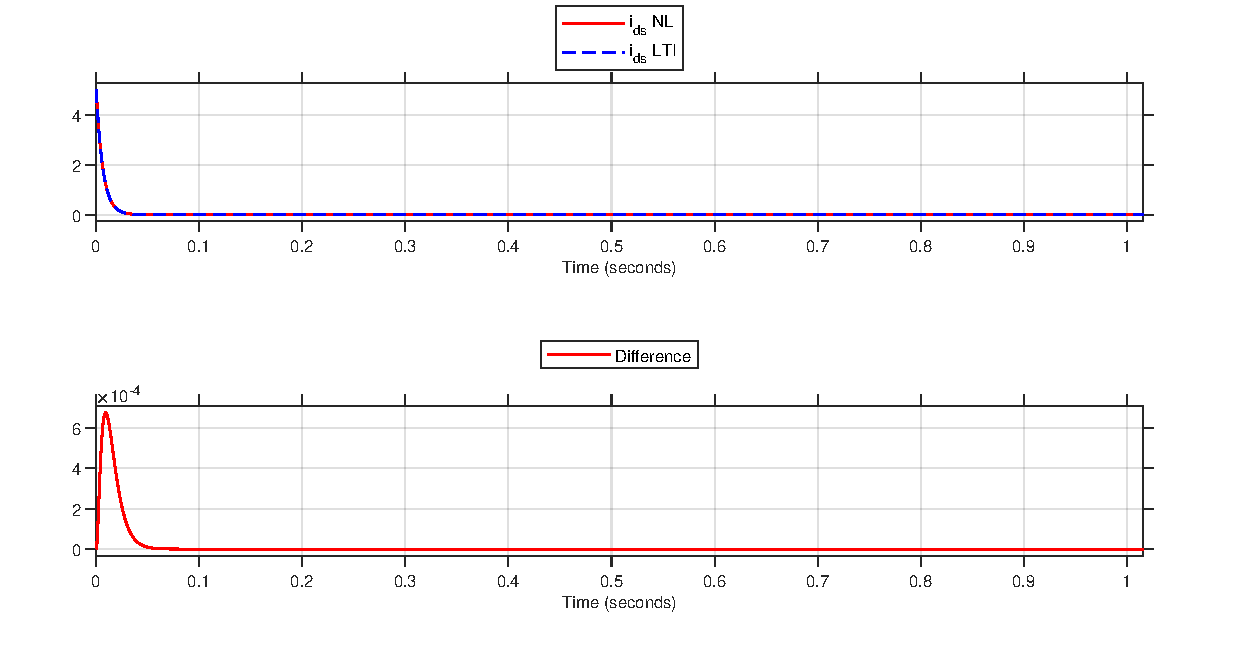
\includegraphics{49-Corriente_ids_5_simulacion_5_1_6.pdf}}
	\end{adjustbox}
	\caption{Diferencia entre la corriente del sistema NL y la del LTI aumentado para $i^r_{ds}(0) = 5A $.}
	\label{Diferencia entre la corriente del sistema NL y la del LTI aumentado para $i^r_{ds}(0) = 5A $}
\end{figure}

\begin{figure}[H]
	\centering
	\begin{adjustbox}{max width=\columnwidth}
		\framebox{\includegraphics{50-Corriente_ids_-5_simulacion_5_1_6.pdf}}
	\end{adjustbox}
	\caption{Diferencia entre la corriente del sistema NL y la del LTI aumentado para $i^r_{ds}(0) = -5A $.}
	\label{Diferencia entre la corriente del sistema NL y la del LTI aumentado para $i^r_{ds}(0) = -5A $}
\end{figure}
Se puede observar que cuando la corriente inicial del eje d es no nula, no hay diferencias notables entre el modelo NL realimentado y el LTI aumentado. Este se debe al desacoplamiento que se hizo entre los ejes q y d.

\paragraph{\textbf{Agregado de consigna de tensión en eje d}}
Se agregó la consigna de tensión ${v^r_{ds}}^* = \pm 1.9596 \, V $ en $t = 0.5 s$ para realizar debilitamiento o reforzamiento de campo. Los resultados obtenidos fueron los siguientes:

\begin{figure}[H]
	\centering
	\begin{adjustbox}{max width=\columnwidth}
		\framebox{\includegraphics{51-Velocidad_deb_ref_campo_simulacion_5_1_6.pdf}}
	\end{adjustbox}
	\caption{Velocidad del motor con ${v^r_{ds}}^* > 0$, ${v^r_{ds}}^* = 0$ y ${v^r_{ds}}^* < 0$.}
	\label{Velocidad del motor con ${v^r_{ds}}^* > 0$, ${v^r_{ds}}^* = 0$ y ${V^r_{ds}}^* < 0$}
\end{figure}

\begin{figure}[H]
	\centering
	\begin{adjustbox}{max width=\columnwidth}
		\framebox{\includegraphics{52-Torque_deb_ref_campo_simulacion_5_1_6.pdf}}
	\end{adjustbox}
	\caption{Torque electromagnético con ${v^r_{ds}}^* > 0$, ${v^r_{ds}}^* = 0$ y ${v^r_{ds}}^* < 0$.}
	\label{Torque electromagnético con ${V^r_{ds}}^* > 0$, ${V^r_{ds}}^* = 0$ y ${V^r_{ds}}^* < 0$}
\end{figure}
En estas gráficas se puede observar el efecto del debilitamiento y reforzamiento del campo. En el primer caso, el debilitamiento del campo provoca un aumento en la velocidad del motor y una disminución del torque. En el segundo caso, el reforzamiento del campo produce el efecto contrario, disminuyendo la velocidad del motor y aumentando el torque. Por otro lado, este tipo de consigna no tiene efecto sobre el sistema LTI equivalente aumentado, ya que en este se desacoplaron los ejes q y d entre sí.

\subsection{\textbf{Modelado, Análisis y Simulación con controlador de movimiento en cascada con modulador de torque equivalente(control vectorial)}}
\label{subsec: Diseño del controlador}

\subsubsection{\textbf{Modulador de torque equivalente(Controlador interno vectorial de corriente/torque)}}
\paragraph{\textbf{Compensación de todas las realimentaciones físicas naturales de estado hacia la entrada}}
Para lograrlo primero se analizaron las ecuaciones del modelo NL del sub-sistema electromagnético:

\begin{align}
	\begin{cases}
		\frac{d i^r_{qs}(t)}{dt} &= -\frac{R_s(t) i^r_{qs}(t)}{L_q} - \frac{P_p \omega_m(t) \left[\lambda'^r_m + L_d i^r_{ds}(t)\right]}{L_q} + \frac{v^r_{qs}(t)}{L_q}\\
		\frac{d i^r_{ds}(t)}{dt} &= -\frac{R_s(t) i^r_{ds}(t)}{L_d} + \frac{L_q P_p \omega_m(t)i^r_{qs}(t)}{L_d}  + \frac{v^r_{ds}(t)}{L_d} \\ 
		\frac{d i_{0s}(t)}{dt}   &= -\frac{R_s(t) i_{0s}(t)}{L_{ls}} + \frac{v_{0s}(t)}{L_{ls}}
	\end{cases}	\label{Ecuaciones NL del subsistema electromagnetico}
\end{align}

Se puede ver que del lado derecho de las ecuaciones tenemos todas las realimentaciones físicas además de las tensiones de entrada. Por lo tanto, para compensar estas realimentaciones, se propusieron las siguientes tensiones como consigna de entrada, en donde las tensiones  ${v^r_{qd0s}(t)}^*$ son las nuevas consignas con las realimentaciones ya compensadas:
 
 \begin{align}
 	v^r_{qs}(t) &= {v^r_{qs}}^*(t) + R_s(t) i^r_{qs}(t) + P_p \omega_m(t) \left[\lambda'^r_m + L_d i^r_{ds}(t)\right] \label{Ecuacion desacoplamientos en vqs}\\
 	v^r_{ds}(t) &= {v^r_{ds}(t)}^* + R_s(t) i^r_{ds}(t) - L_q P_p \omega_m(t)i^r_{qs}(t) \label{Ecuacion desacoplamientos en vds}\\ 
 	v_{0s}(t)   &= {v_{0s}(t)}^* + R_s(t) i_{0s}(t) \label{Ecuacion desacoplamientos en v0s}
 \end{align}

Al reemplazar las ecuaciones \eqref{Ecuacion desacoplamientos en vqs}, \eqref{Ecuacion desacoplamientos en vds} y \eqref{Ecuacion desacoplamientos en v0s} en la \cref{Ecuaciones NL del subsistema electromagnetico}, se cancelan los términos de las realimentaciones y se obtiene el siguiente modelo:

\begin{align}
	\begin{cases}
		\frac{d i^r_{qs}(t)}{dt} &= \frac{{v^r_{qs}(t)}^*}{L_q}\\
		\frac{d i^r_{ds}(t)}{dt} &= \frac{{v^r_{ds}(t)}^*}{L_d} \\ 
		\frac{d i_{0s}(t)}{dt}   &= \frac{{v_{0s}(t)}^*}{L_{ls}}
	\end{cases}	\label{Ecuaciones del subsistema electromagnetico sin realimentaciones fisicas}
\end{align}

De esta manera, se obtiene un sistema lineal en el cual existe acceso directo a las corrientes, sin realimentaciones. Cabe destacar que con este método solo se compensaron, y no se eliminaron completamente, los efectos que provocan las realimentaciones, ya que  estas se deben al comportamiento físico propio del sistema. Además se está suponiendo que se tienen los sensores necesarios para medir los estados a realimentar.

\paragraph{\textbf{Diseño de lazos de control de corrientes $\mathbf{{i}^r_{qd0s}(t)}$}}
Luego de haber desacoplado todas las realimentaciones, se incorporaron lazos de control de corriente solamente proporcional (con polos ubicados en $p_{i}=-5000\dfrac{rad}{s}$), con consignas de corriente en lugar de tensiones y así lograr un control más preciso del torque.
Para lograrlo, se definieron las consignas de tensión  ${v^r_{qd0s}(t)}^*$ de la siguiente manera:
 \begin{align}
	{v^r_{qs}}^*(t) &= R_q \left[ {i^r_{qs}(t)}^* - i^r_{qs}(t) \right] \label{Ecuacion control corrinte iq}\\
	{v^r_{ds}(t)}^* &= R_d \left[ {i^r_{ds}(t)}^* - i^r_{ds}(t) \right] \label{Ecuacion control corrinte id}\\ 
	{v_{0s}(t)}^*   &= R_0 \left[ {i_{0s}(t)}^* - i_{0s}(t) \right] \label{Ecuacion control corrinte i0}
\end{align}
En donde las consignas de tensión son proporcionales al error de corriente, y las constantes de proporcionalidad son resistencias con unidades en ohm.

Para determinar el valor de las ganancias se reemplazaron las ecuaciones \eqref{Ecuacion control corrinte iq}, \eqref{Ecuacion control corrinte id} y \eqref{Ecuacion control corrinte i0} en la \cref{Ecuaciones del subsistema electromagnetico sin realimentaciones fisicas}, y luego se encontraron las funciones de transferencia del sistema resultante:

\begin{align}
	\begin{cases}
		\frac{d i^r_{qs}(t)}{dt} &= \frac{ R_q \left[ {i^r_{qs}(t)}^* - i^r_{qs}(t))\right]}{L_q}\\
		\frac{d i^r_{ds}(t)}{dt} &= \frac{R_d \left[ {i^r_{ds}(t)}^* - i^r_{ds}(t) \right]}{L_d} \\ 
		\frac{d i_{0s}(t)}{dt}   &= \frac{R_0 \left[ {i_{0s}(t)}^* - i_{0s}(t) \right]}{L_{ls}}
	\end{cases}	\label{Ecuaciones lazos de control de corriente}
\end{align}

\begin{align}
	\begin{cases}
		s{I}^r_{qs}(s) &= \frac{ R_q \left[ {I^r_{qs}(s)}^* - I^r_{qs}(s))\right]}{L_q}\\
		s{I}^r_{ds}(s) &= \frac{R_d \left[ {I^r_{ds}(s)}^* - I^r_{ds}(s) \right]}{L_d} \\ 
		s{I}_{0s}(s)   &= \frac{R_0 \left[ {I_{0s}(s)}^* - I_{0s}(s) \right]}{L_{ls}}
	\end{cases}	\label{Ecuaciones Laplace lazos de control de corriente}
\end{align}

\begin{align}
	\begin{cases}
		G_{{I}^r_{qs}}(s) &=\frac{{I}^r_{qs}(s)}{{I^r_{qs}(s)}^*} =\frac{1}{\frac{L_q}{R_q} s + 1}\\
		G_{{I}^r_{ds}}(s) &=\frac{{I}^r_{ds}(s)}{{I^r_{ds}(s)}^*} = \frac{1}{\frac{L_d}{R_d} s + 1}\\ 
		G_{{I}_{0s}}(s)   &=\frac{{I}_{0s}(s)}{{I_{0s}(s)}^*} = \frac{1}{\frac{L_{ls}}{R_0} s + 1}
	\end{cases}	\label{Funciones de Transferencia de lazos de control de corriente}
\end{align}
Al observar estas funciones de transferencia, se puede ver que contienen un solo polo:

\begin{align}
	\frac{L_q}{R_q} s + 1 &= 0 \Rightarrow s = -\frac{R_q}{L_q}\\
	\frac{L_{d}}{R_d} s + 1 &=0 \Rightarrow s = -\frac{R_d}{L_d}\\ 
	\frac{L_{ls}}{R_0} s + 1  &=0 \Rightarrow s = -\frac{R_0}{L_{ls}}
\end{align}
Al posicionar los polos en $p_{i}=-5000 \, frac{rad}{s}$, se obtuvieron las siguientes ecuaciones para las ganancias:

\begin{align}
	R_q &= 5000 L_q = 29 \, \Omega\\
	R_d &= 5000 L_d = 33 \, \Omega\\ 
	R_0 &= 5000 L_{ls} = 4 \, \Omega
\end{align}

\paragraph{\textbf{Incorporación de consigna de torque}}
Luego de haber incorporado los lazos de control de corriente, se hizo la realimentación necesaria para pasar de consignas de corrientes a una consigna de torque. Para esto, primero se analizó la ecuación del torque electromagnético, de donde podemos despejar la consigna de corriente ${i^r_{qs}(t)}^*$:

\begin{align}
	T_m(t) &= \frac{3}{2} P_p [\lambda'^r_{m} {i^r_{qs}(t)}^* + (L_d - L_q) i^r_{ds}(t) {i^r_{qs}(t)}^*] \label{torque electromagnetico 2}\\
	{i^r_{qs}(t)}^* &= \frac{T_m(t)}{\frac{3}{2} P_p [\lambda'^r_{m} + (L_d - L_q) i^r_{ds}(t)]}
\end{align}
 Además, se incorporó el término de fricción para compensar este efecto:
 \begin{align}
 	{i^r_{qs}(t)}^* &= \frac{{T_m(t)}^* + b_{eq} \omega_m(t) }{\frac{3}{2} P_p [\lambda'^r_{m} + (L_d - L_q) i^r_{ds}(t)]}
 \end{align}
	
\paragraph{\textbf{Compensación del torque de carga por gravedad}}
Al analizar la ecuación de estado de la velocidad, luego de haber reemplazado la consigna de corriente,
\cref{ecuacion de estado wm con consigna de torque}, se pudo ver que es posible compensar el término del torque de carga por gravedad, proponiendo la consigna de torque
de la \cref{consigna de torque para desacoplar carga por gravedad}

\begin{equation}
	\frac{d \omega_m(t)}{dt} = \frac{{T_m(t)}^*}{ J_{eq}} - \frac{k_l \sin \left( \frac{\theta_m}{r}\right) }{r J_{eq}} - \frac{T_d(t)}{r J_{eq}}
	\label{ecuacion de estado wm con consigna de torque}
\end{equation}

\begin{equation}
	{T_m(t)}^* = {T_m(t)}^{*'} + \frac{k_l \sin \left( \frac{\theta_m}{r}\right) }{r}
	\label{consigna de torque para desacoplar carga por gravedad}
\end{equation}

La \cref{ecuacion de estado wm con consigna de torque} queda de la siguiente manera:
\begin{equation}
	\frac{d \omega_m(t)}{dt} = \frac{{T_m(t)}^{*'}}{ J_{eq}}- \frac{T_d(t)}{r J_{eq}}
	\label{ecuacion de estado wm sin gravedad}
\end{equation}

\subsubsection{\textbf{Controlador externo de movimiento: posición/velocidad}}
Para mejorar la dinámica del sistema, eliminar el error de estado estacionario y poder seguir consignas de posición/velocidad se añadió un controlador externo de posición tipo PID que determine las consignas de torque $T_m(t)^{*'}$ necesarias:

\begin{equation}
	{T_m(s)}^{*'} = \left[ {\omega}_m^{*}(s)-{\omega}_m(s)\right] b_a + \frac{\left[ {\omega}_m^{*}(s)-{\omega}_m(s)\right]}{s} K_{sa} + \frac{\left[ {\omega}_m^{*}(s)-{\omega}_m(s)\right]}{s^2} K_{sia}
\end{equation}
\begin{align}
	J_{eq} s^2 \Theta_m(s) &= {T_m(s)}^{*'}- \frac{T_d(s)}{r }  \\
	J_{eq} s^2 \Theta_m(s) &= \left[ {\Theta}_m^{*}(s)-{\Theta}_m(s)\right] \left( b_a s + K_{sa} + \frac{1}{s} K_{sia}\right)  - \frac{T_d(s)}{r } \\
	\left( J_{eq} s^3 + b_a s^2 + K_{sa} s +  K_{sia}\right) \Theta_m &=   \left( b_a s^2 + K_{sa} s + K_{sia}\right) {\Theta}_m^{*}(s)  - \frac{T_d(s)}{r} s \\ 
	\Theta_m(s) &= \frac{ b_a s^2 + K_{sa} s + K_{sia}}{J_{eq} s^3 + b_a s^2 + K_{sa} s +  K_{sia}} {\Theta}_m^{*}(s)  - \frac{s}{J_{eq} s^3 + b_a s^2 + K_{sa} s +  K_{sia}} \frac{T_d(s)}{r} \\
	G_{{\Theta}_m^{*}}(s) &= \frac{ b_a s^2 + K_{sa} s + K_{sia}}{J_{eq} s^3 + b_a s^2 + K_{sa} s +  K_{sia}} \\
	G_{T_l}(s) &= -\frac{s}{J_{eq} s^3 + b_a s^2 + K_{sa} s +  K_{sia}}
\end{align}
Se puede observar, a partir del teorema del valor final, que al colocar una acción integral, desaparece el error de estado estacionario para una perturbación escalón unitario:

\begin{itemize}
	\item Si $K_{sia}=0 \: \land \: \frac{T_d(s)}{r} = \frac{1}{s} \: \land \: {\Theta}_m^{*}(s) = 0 \Rightarrow \lim_{t \to \infty} \theta_m(t) = \lim_{s \to 0} s\Theta_m(s) = -\frac{1}{K_{sa}} $ 
	\item Si $K_{sia}=0 \: \land \: \frac{T_d(s)}{r} = 0 \: \land \: {\Theta}_m^{*}(s) = \frac{1}{s} \Rightarrow \lim_{t \to \infty} \theta_m(t) = \lim_{s \to 0} s\Theta_m(s) = 1 $
	\item Si $K_{sia}\neq0 \: \land \: \frac{T_d(s)}{r} = \frac{1}{s} \: \land \: {\Theta}_m^{*}(s) = 0 \Rightarrow \lim_{t \to \infty} \theta_m(t) = \lim_{s \to 0} s\Theta_m(s) = 0$
	\item Si $K_{sia}\neq0 \: \land \: \frac{T_d(s)}{r} = 0 \: \land \: {\Theta}_m^{*}(s) = \frac{1}{s} \Rightarrow \lim_{t \to \infty} \theta_m(t) = \lim_{s \to 0} s\Theta_m(s) = 1 $
\end{itemize}

Para encontrar los valores de las ganancias del controlador PID, se utilizo el método de sintonía serie, con $n=2.5$ y $\omega_{pos}=800\frac{rad}{s}$ y $J_{eq}$ nominal. Donde se comparó el polinomio característico, \cref{polinomio característico}, con el polinomio de la \cref{polinomio sintonía serie}, 
obteniéndose las ganancias indicadas en la \cref{ganancias PID}.

\begin{equation}
	P(s) =  s^3 + \frac{b_a}{J_{eq}} s^2 + \frac{K_{sa}}{J_{eq}} s + \frac{K_{sia}}{J_{eq}}
	\label{polinomio característico}
\end{equation}

\begin{equation}
	P(s) =  s^3 + n \omega_{pos} s^2 + n {\omega_{pos}}^2 s + {\omega_{pos}}^3 
	\label{polinomio sintonía serie}
\end{equation}

\begin{align}
	b_a &=  n \, \omega_{pos} \, J_{eq}= 0.0396 \, \frac{Nm}{rad/s} \\
	K_{sa} &=  n \, {\omega_{pos}}^2 \, J_{eq}= 31.6556 \, \frac{Nm}{rad}\\
	K_{sia} &= {\omega_{pos}}^3 \, J_{eq}= 10130 \, \frac{Nm}{rad \, s}
	\label{ganancias PID}
\end{align}

Los polos para estos valores de ganancias serían los siguientes:
\begin{align}
	s_1 &= -800 \\
	s_2 &=  -600 + i \, 529.15\\
	s_3 &=  -600 - i \, 529.15
\end{align}

Finalmente, en la \cref{mapa de polos-ceros controlador-planta} se muestra el mapa de polos/zeros del controlador de movimiento
en comparación con el mapa de polos/ceros de la planta a lazo abierto cuando hay una variación continua de $J_l$ en todo su rango
sin considerar la variación de $b_l$ (que se considera en su valor nominal) ya que no determina el valor de los polos del controlador de movimiento y tiene un 
efecto despreciable en el cambio de polos de la planta a lazo abierto.

\begin{figure}[H]
	\centering
	\begin{adjustbox}{max width=\columnwidth}
		\framebox{\includegraphics{53-mapa_polos_ceros_controlador_vs_planta.pdf}}
	\end{adjustbox}
	\caption{Mapa de polos/zeros controlador de movimiento-planta.}
	\label{mapa de polos-ceros controlador-planta}
\end{figure}

Al comparar los polos de los lazos de corriente con los del controlador de posición, se observa que estos últimos tienen una frecuencia al menos seis veces menor que los primeros.


\subsubsection{\textbf{Incorporación de observador de estado de orden reducido para parte mecánica}}
Como en este controlador se ha optado por realimentar la velocidad, para evitar la utilización de derivadores, y dado que se cuenta con un encoder para medir posición del eje, fue necesario implementar un observador de estado reducido para poder realimentar la velocidad angular del motor. Se aclara que las corrientes no son observadas, ya que se cuenta con sensores de corriente.

Para diseñar el observador, se analizó el sub-sistema mecánico resultante luego de todas las compensaciones:
\begin{align}
	\begin{cases}
		\frac{d\theta_m(t)}{dt} ={\omega}_m(t)\\
		\frac{d\omega_m(t)}{dt} = \frac{{T_m(t)}^{*'}}{ J_{eq}}- \frac{T_d(t)}{r J_{eq}}
	\end{cases}\label{ecuacion de subsistema mecanico compensado}
\end{align}
 Equivalentemente, en forma de espacio de estados:
 
\begin{align}
	\begin{cases}
		\begin{bmatrix}
			\frac{d\theta_m(t)}{dt} \\ 
			\frac{d\omega_m(t)}{dt}
		\end{bmatrix} &= 
		\begin{bmatrix}
			0 & 1 \\ 
			0 & 0
		\end{bmatrix}
		\begin{bmatrix}
			{\theta}_m(t) \\ 
			{\omega}_m(t)
		\end{bmatrix} + 
		\begin{bmatrix}
			0 \\ 
			\frac{1}{J_{eq}}
		\end{bmatrix} {T_m(t)}^{*'} +
		\begin{bmatrix}
			0 \\ 
			-\frac{1}{r J_{eq}}
		\end{bmatrix} T_d(t)\\
		y(t) &= \begin{bmatrix}
			1 & 0
		\end{bmatrix} \begin{bmatrix}
		{\theta}_m(t) \\ 
		{\omega}_m(t)
		\end{bmatrix}
	\end{cases}\label{ecuacion matricial de subsistema mecanico compensado}
\end{align}
Al asumir un funcionamiento ideal, las ecuaciones del observador quedan similares a las del sistema, con el agregado de un término proporcional al error entre la salida del sistema real y la estimada:
\begin{align}
	\begin{cases}
		\begin{bmatrix}
			\frac{d \tilde{\theta}_m(t)}{dt} \\ 
			\frac{d \tilde{\omega}_m(t)}{dt}
		\end{bmatrix} &= 
		\begin{bmatrix}
			0 & 1 \\ 
			0 & 0
		\end{bmatrix}
		\begin{bmatrix}
			{\tilde{\theta}}_m(t) \\ 
			{\tilde{\omega}}_m(t)
		\end{bmatrix} + 
		\begin{bmatrix}
			0 \\ 
			\frac{1}{J_{eq}}
		\end{bmatrix} {T_m(t)}^{*'} + 
		\begin{bmatrix}
			K_{\theta} \\
			K_{\omega}
		\end{bmatrix} \left(y(t) - \tilde{y}(t) \right) \\
		\tilde{y}(t) &= \begin{bmatrix}
			1 & 0
		\end{bmatrix} 
		\begin{bmatrix}
			{\tilde{\theta}}_m(t) \\ 
			{\tilde{\omega}}_m(t)
		\end{bmatrix}
	\end{cases}\label{ecuacion matricial de observador}
\end{align}
Al evaluar la dinámica del error de estimación obtenemos las siguientes ecuaciones: 
\begin{align}
	\frac{d \mathbf{e}(t)}{dt} &= \frac{d \mathbf{x}(t)}{dt} - \frac{d \mathbf{\tilde{x}} (t)}{dt}\\
	\frac{d \mathbf{e}(t)}{dt} &= A {\mathbf{x}(t)} + B_c {T_m(t)}^{*'} + B_d T_d(t) - \left( A \mathbf{\tilde{x} (t)} + B_c {T_m(t)}^{*'} + K C \left(\mathbf{x(t)} - \mathbf{\tilde{x} (t)} \right) \right) \\
	\frac{d \mathbf{e}(t)}{dt} &= \left(A - KC \right) {\mathbf{e(t)}} + B_d T_d(t)\label{dinamica del error de estimacion}
\end{align}
En donde la matriz que gobierna la dinámica es $\left(A - KC \right)$, por lo que se busca su polinomio característico:
\begin{align}
	p(s) = det\left(s I - \left( A - KC\right)  \right) = det\left(\begin{bmatrix}
		s + K_{\theta} & -1 \\ 
		K_{\omega} & s
	\end{bmatrix}  
	 \right) = s^2 + K_{\theta} s + K_{\omega} \label{polinomeo caracteristico de observador}
\end{align}

Luego, se planteó el polinomio de segundo orden con polos deseados reales e iguales en $p_{obs1,2} = -3200 \frac{rad}{s}$ para no interferir con el controlador y asegurar un decaimiento rápido del error de observación:
\begin{align}
	p(s) = \left( s + 3200\right) ^2 = s^2 + 6400 s + 10240000\label{polinomeo caracteristico de observador deseado}
\end{align}
Al comparar ambos polinomios obtenemos los valores de las ganancias del observador:
\begin{align}
	K_{\theta} &= 6400 \, seg^{-1}\label{ganacia de posicion de observador}\\
	K_{\omega} &= 10240000 \, seg^{-2}\label{ganacia de velocidad de observador}
\end{align}
El diagrama de bloques resultante queda de la siguiente manera:
\begin{figure}[H]
	\centering
	\begin{adjustbox}{max width=\columnwidth,scale=0.8}
		\framebox{\includegraphics{54-Observador.pdf}}
	\end{adjustbox}
	\caption{Diagrama de bloques del observador de estado de orden reducido.}
	\label{Diagrama de bloques del observador de estado de orden reducido}
\end{figure}
Donde se puede observar que se le añadió el modelo equivalente del modulador de torque.
\subsubsection{\textbf{Simulación en tiempo continuo con modelo no lineal completo}}
Para poder realizar la simulación en tiempo continuo, se integraron todos los bloques del controlador, en un solo diagrama de bloques, separando el controlador de la planta. Además se pueden visualizar el modulador de tensión y los sensores con ganancias unitarias:
\begin{figure}[H]
	\centering
	\begin{adjustbox}{max width=\columnwidth}
		\framebox{\includegraphics{55-Controlador_completo}}
	\end{adjustbox}
	\caption{Diagrama de bloques del controlador completo.}
	\label{Diagrama de bloques del controlador completo}
\end{figure}

%\begin{figure}[H]
	%\centering
	%\begin{adjustbox}{max width=\columnwidth}
%		\framebox{\includegraphics{9-Planta_completa.pdf}}
	%\end{adjustbox}
	%\caption{Diagrama de bloques de la planta}
	%\label{Diagrama de bloques de la planta}
%\end{figure}

\paragraph{\textbf{Seguimiento de consignas de movimiento}}
La consigna para el sistema será la posición angular de la artículación del brazo \ensuremath{{q^*}(t) \equiv \frac{1}{r} {\theta^*_m}(t)}, que seguirá un perfil trapezoidal con las siguientes características:
\begin{equation}
	{q^*}(1)=0 \: [rad] \longrightarrow {q^*}(6)=2 \pi \: [rad] \longrightarrow {q^*}(11)=2 \pi \: [rad]\longrightarrow {q^*}(16)=0 \: [rad]
\end{equation}
Los resultados de la simulación fueron los siguientes:

\begin{figure}[H]
	\centering
	\begin{adjustbox}{scale=0.5,max width=\columnwidth}
		\framebox{\includegraphics{56-grafica_posicion_vs_posicionconsigna}}
	\end{adjustbox}
	\caption{Gráfica de posición angular consigna y medida.}
	\label{Grafica de posicion angular consigna y medida }
\end{figure}
\begin{figure}[H]
	\centering
	\begin{adjustbox}{scale=0.5,max width=\columnwidth}
		\framebox{\includegraphics{57-grafica_error _posicion_vs_posicionconsigna}}
	\end{adjustbox}
	\caption{Gráfica del error entre posición angular consigna y medida.}
	\label{Grafica del error entre posicion angular consigna y medida }
\end{figure}

\begin{figure}[H]
	\centering
	\begin{adjustbox}{scale=0.5,max width=\columnwidth}
		\framebox{\includegraphics{58-grafica__detalle_error _posicion_vs_posicionconsigna}}
	\end{adjustbox}
	\caption{Detalle del error entre posición angular consigna y medida.}
	\label{Detalle del error entre posición angular consigna y medida }
\end{figure}
Se observa que la consigna se cumple prácticamente sin errores. Sin embargo, los perfiles de velocidad presentan una forma escalonada.
\begin{figure}[H]
	\centering
	\begin{adjustbox}{max width=\columnwidth}
		\framebox{\includegraphics{59-grafica_velocidad_m_vs_consigna_velocidad_m_vs_velocidad_e}}
	\end{adjustbox}
	\caption{Gráficas de velocidad del motor consigna, medida y estimada.}
	\label{Gráficas de velocidad del motor consigna, medida y estimada}
\end{figure}
Estos perfiles de velocidad implican aceleraciones impulsivas, que el sistema trata de cumplir con tensiones, corrientes y torques elevados.
\begin{figure}[H]
	\centering
	\begin{adjustbox}{scale=0.5,max width=\columnwidth}
		\framebox{\includegraphics{60-grafica_torque_y_corriente_iqs}}
	\end{adjustbox}
	\caption{Gráfica de torque electromagnético y corriente $i^r_{qs}(t)$.}
	\label{Gráfica de torque electromagnético y corriente $i_{qs}$}
\end{figure}

\begin{figure}[H]
	\centering
	\begin{adjustbox}{scale=0.5,max width=\columnwidth}
		\framebox{\includegraphics{61-grafica_corrientes_abc}}
	\end{adjustbox}
	\caption{Gráficas de corrientes abc.}
	\label{Gráficas de corrientes $i_{abc}$}
\end{figure}

\begin{figure}[H]
	\centering
	\begin{adjustbox}{scale=0.5,max width=\columnwidth}
		\framebox{\includegraphics{62-grafica_tensiones_abc}}
	\end{adjustbox}
	\caption{Gráficas de tensiones abc.}
	\label{Gráficas de tensiones abc}
\end{figure}

\paragraph{\textbf{Rechazo de perturbaciones}} 
Se evaluó el comportamiento del sistema ante torques de perturbación del tipo escalón, como la que se observa en la siguiente figura, considerando valores nominales y variación máxima de los parámetros de carga mecánica física.
\begin{figure}[H]
	\centering
	\begin{adjustbox}{scale=0.47,max width=\columnwidth}
		\framebox{\includegraphics{63-Torque_de_perturbacion}}
	\end{adjustbox}
	\caption{Torque de perturbación.}
	\label{Torque de perturbación}
\end{figure}
Los resultados fueron los siguientes:
\begin{figure}[H]
	\centering
	\begin{adjustbox}{scale=0.53,max width=\columnwidth}
		\framebox{\includegraphics{64-grafica_error _posicion_vs_posicionconsigna_con_perturbacion}}
	\end{adjustbox}
	\caption{Error entre  posición consigna y medida.}
	\label{Error entre  posición consigna y medida}
\end{figure}

\begin{figure}[H]
	\centering
	\begin{adjustbox}{scale=0.53,max width=\columnwidth}
		\framebox{\includegraphics{65-Error_entre_posicion_medida_y_posicion_observada_ante_perturbacion}}
	\end{adjustbox}
	\caption{Error entre  posición medida y estimada.}
	\label{Error entre  posición medida y estimada}
\end{figure}
Se observa que al aplicar una perturbación, apareció un error de estado estacionario entre las posiciones consigna, medida y observada.
\subsubsection{\textbf{Verificación de desempeño y mejoras}}
\paragraph{\textbf{Verificación de las especificaciones de operación}}Al comparar los valores obtenidos en las simulaciones, con los límites de operación dados por el fabricante de la máquina, se obtuvieron los siguientes resultados:

\begin{table}[H]
	\centering
	\begin{tabular}{|c|cc|cc|}
		\hline
		\multirow{2}{*}{} & \multicolumn{2}{c|}{Valores obtenidos de simulación} & \multicolumn{2}{c|}{Especificaciones de operación}   \\ \cline{2-5} 
		& \multicolumn{1}{c|}{Régimen Continuo} & Valores Pico & \multicolumn{1}{c|}{Régimen Continuo} & Valores Pico \\ \hline
		Tensión de linea         & \multicolumn{1}{c|}{7.5 V}                & 2374.9 V            & \multicolumn{1}{c|}{24 V}                & -            \\ \hline
		Corriente         & \multicolumn{1}{c|}{0.3 A}                & 67.5 A            & \multicolumn{1}{c|}{0.4 A}                & 2 A            \\ \hline
		Torque motor            & \multicolumn{1}{c|}{0.04 Nm}                & 4.9 Nm            & \multicolumn{1}{c|}{0.142 Nm}               & 0.375 Nm           \\ \hline
		Velocidad angular del motor         & \multicolumn{1}{c|}{150.8 rad/s}               & 209.4 rad/s           & \multicolumn{1}{c|}{691.15 rad/s }               & -           \\ \hline
	\end{tabular}
\end{table}

Se puede ver que los valores de tensión, corriente y torque obtenidos en la simulación superan los límites especificados en las condiciones de operación, debido a los impulsos de aceleraciones que requiere la consigna. 

Para solucionar este problema, se propuso un perfil de posición alternativo que sigue cumpliendo con los requisitos de posicionamiento y tiempo, pero en lugar de rampas, se utilizan polinomios de quinto grado. Con esta modificación, las consignas de aceleración se transforman en funciones cúbicas en lugar de impulsos, lo que resulta en un cambio suave en la tasa de aceleración (jerk). Esto logra una reducción de vibraciones en una aplicación real y una mayor durabilidad del sistema. Para determinar los coeficientes de estos polinomios, es necesario conocer la posición, velocidad y aceleración en los puntos extremos del perfil.
\begin{align}
	q*(t) &= at^5 + bt^4 + ct^3 + dt^2 + et + f  \\
	\frac{d q*(t)}{dt} &=  5at^4 + 4bt^3 + 3ct^2 + 2dt + e \\
	\frac{d^2 q*(t)}{dt^2} &=  20at^3 + 12bt^2 + 6ct + 2d\\
\end{align}
Las aceleraciones y velocidades en los extremos serán cero, mientras que las posiciones serán las mismas que en la consigna anterior. Por lo que para la primer giro queda el siguiente sistema de ecuaciones:
\begin{align}
	\begin{cases}
		0[rad]  &= a_1(1 [s])^5 + b_1(1 [s])^4 + c_1(1 [s])^3 + d_1(1 [s])^2 + e_1(1 [s]) + f_1 \\
		2\pi [rad] &= a_1(6 [s])^5 + b_1(6 [s])^4 + c_1(6 [s])^3 + d_1(6 [s])^2 + e_1(6 [s]) + f_1  \\
		0[rad/s] &= 5a_1(1 [s])^4 + 4b_1(1 [s])^3 + 3c_1(1 [s])^2 + 2d_1(1 [s]) + e_1 \\
		0[rad/s] &= 5a_1(6 [s])^4 + 4b_1(6 [s])^3 + 3c_1(6 [s])^2 + 2d_1(6 [s]) + e_1 \\
		0[rad/s^2] &= 20a_1(1 [s])^3 + 12b_1(1 [s])^2 + 6c_1(1 [s]) + 2d_1 \\
		0[rad/s^2] &= 20a_1(6 [s])^3 + 12b_1(6 [s])^2 + 6c_1(6 [s]) + 2d_1
	\end{cases}
\end{align}

Y para el giro de regreso:
\begin{align}
	\begin{cases}
		0[rad]  &= a_2(11 [s])^5 + b_2(11 [s])^4 + c_2(11 [s])^3 + d_2(11 [s])^2 + e_2(11 [s]) + f_2 \\
		2\pi [rad] &= a_2(16 [s])^5 + b_2(16 [s])^4 + c_2(16 [s])^3 + d_2(16 [s])^2 + e_2(16 [s]) + f_2  \\
		0[rad/s] &= 5a_2(11 [s])^4 + 4b_2(11 [s])^3 + 3c_2(11 [s])^2 + 2d_2(11 [s]) + e_2 \\
		0[rad/s] &= 5a_2(16 [s])^4 + 4b_2(16 [s])^3 + 3c_2(16 [s])^2 + 2d_2(16 [s]) + e_2 \\
		0[rad/s^2] &= 20a_2(11 [s])^3 + 12b_2(11 [s])^2 + 6c_2(11 [s]) + 2d_2 \\
		0[rad/s^2] &= 20a_2(16 [s])^3 + 12b_2(16 [s])^2 + 6c_2(16 [s]) + 2d_2
	\end{cases}
\end{align}

Al resolver estos sistemas de ecuaciones, se obtuvieron los siguientes polinomios:
\begin{align}
	q*_1(t) &= 0.0121t^5 - 0.2111t^4 + 1.2265t^3 - 2.5334t^2 + 2.1715t - 0.6655\\
	q*_2(t) &= -0.0121t^5 + 0.8143t^4 - 21.7348t^3 + 286.6339t^2 - 1868.4283t + 4826.0010
\end{align}
 
Por lo que la consigna resultante fue:
\begin{align}
	q*(t) =
	\begin{cases}
		0  &  t<1 \\
		 0.0121t^5 - 0.2111t^4 + 1.2265t^3 - 2.5334t^2 + 2.1715t - 0.6655  &  1 \leq t \leq 6 \\
		2\pi  &  6 < t < 11 \\
		-0.0121t^5 + 0.8143t^4 - 21.7348t^3 + 286.6339t^2 - 1868.4283t + 4826.0010  &  11 \leq t \leq 16 \\
		0  &  t>16
	\end{cases}
\end{align}

\begin{figure}[H]
	\centering
	\begin{adjustbox}{max width=\columnwidth}
		\framebox{\includegraphics{66-pos_vel_acel_suaves}}
	\end{adjustbox}
	\caption{Nueva consigna de posición, velocidad, aceleración.}
	\label{Nueva consigna de posición, velocidad, aceleración}
\end{figure}

Al realizar nuevamente la simulación con esta nueva consigna se obtuvieron las siguientes gráficas.
\begin{figure}[H]
	\centering
	\begin{adjustbox}{scale=0.5,max width=\columnwidth}
		\framebox{\includegraphics{67-grafica_tensiones_abc_nuevas}}
	\end{adjustbox}
	\caption{Tensiones abc con consigna suave.}
	\label{Tensiones abc con consigna suave}
\end{figure}

\begin{figure}[H]
	\centering
	\begin{adjustbox}{scale=0.5,max width=\columnwidth}
		\framebox{\includegraphics{68-grafica_corrientes_abc_nueva}}
	\end{adjustbox}
	\caption{Corrientes abc con consigna suave.}
	\label{Corrientes abc con consigna suave}
\end{figure}

\begin{figure}[H]
	\centering
	\begin{adjustbox}{scale=0.5,max width=\columnwidth}
		\framebox{\includegraphics{69-grafica_torque_nueva}}
	\end{adjustbox}
	\caption{Torque electromagnético con consigna suave.}
	\label{Torque electromagnético con consigna suave}
\end{figure}
Se puede apreciar que los valores de las variables ahora se encuentran dentro de los límites permitidos. Dado que estos valores están muy por debajo de los límites especificados por el fabricante, la máquina se podría exigir más, utilizando consignas más rápidas.
\paragraph{\textbf{Mejoras en el observador de estado}} 
Como se observó en las simulaciones, existe un error de estado estacionario entre la posición medida del motor y la estimada por el observador cuando se aplica un torque de perturbación. Este error se debe a que el observador no considera dichas perturbaciones y además se comporta como un controlador PD. Si las perturbaciones fueran medibles, se podrían incorporar al observador como entradas; sin embargo, la implementación de un medidor de torque resultaría muy costosa. Por lo tanto, se optó por agregar una acción integral al observador para que se comporte como un controlador PID y poder eliminar este error.

El modelo del observador quedó de la siguiente forma.
\begin{align}
	\begin{cases}
		\begin{bmatrix}
			\frac{d \tilde{\theta}_m(t)}{dt} \\ 
			\frac{d \tilde{\omega}_m(t)}{dt} \\
			\frac{d \tilde{z}(t)}{dt}
		\end{bmatrix} &= 
		\begin{bmatrix}
			0 & 1 & 0\\ 
			0 & 0 & 1 \\
			0 & 0 & 0
		\end{bmatrix}
		\begin{bmatrix}
			{\tilde{\theta}}_m(t) \\ 
			{\tilde{\omega}}_m(t) \\
			\tilde{z}(t)
		\end{bmatrix} + 
		\begin{bmatrix}
			0 \\ 
			\frac{1}{J_{eq}}\\
			0
		\end{bmatrix} {T_m(t)}^{*'} + 
		\begin{bmatrix}
			K_{\theta} \\
			K_{\omega}\\
			K_{i}
		\end{bmatrix} \left(y(t) - \tilde{y}(t) \right) \\
		\tilde{y}(t) &= \begin{bmatrix}
			1 & 0 & 0
		\end{bmatrix} 
		\begin{bmatrix}
			{\tilde{\theta}}_m(t) \\ 
			{\tilde{\omega}}_m(t) \\
			\tilde{z}(t)
		\end{bmatrix}
	\end{cases}\label{ecuacion matricial de observador nuevo}
\end{align}
Como el modelo cambió respecto al observador PD, se calcularon nuevamente las ganancias, determinando el polinomio característico del sistema y comparándolo con el deseado. Para simplificar, el nuevo polo se coloco en la misma posición que los anteriores.
\begin{align}
	p(s) = det\left(s I - \left( A - KC\right)  \right) = det\left(\begin{bmatrix}
		s + K_{\theta} & -1 & 0\\ 
		K_{\omega} & s & -1 \\
		K_{i} & 0 & s
	\end{bmatrix}  
	\right) = s^3 + K_{\theta} s^2 + K_{\omega} s + K_{i} \label{polinomeo caracteristico de observador nuevo}
\end{align}

\begin{align}
	p(s) = \left( s + 3200\right) ^3 = s^3 + 9600 s^2 + 3(3200)^2 s + (3200)^3\label{polinomeo caracteristico de observador nuevo deseado}
\end{align}

\begin{align}
	K_{\theta} &= 9600 \, seg^{-1} \label{ganacia de posicion de observador nuevo}\\
	K_{\omega} &= 3(3200)^2 seg^{-2} \label{ganacia de velocidad de observador nuevo}\\
	K_{i} &= (3200)^3 seg^{-3} \label{ganacia integral de observador nuevo}
\end{align}
El diagrama de bloques resultante es el siguiente:
\begin{figure}[H]
	\centering
	\begin{adjustbox}{scale=0.5,max width=\columnwidth}
		\framebox{\includegraphics{70-Observador_con_integrador.pdf}}
	\end{adjustbox}
	\caption{Diagrama del bloques del observador con acción integral.}
	\label{Diagrama del bloques del observador con acción integrale}
\end{figure}
Con esta modificación, el error de estado estacionario desaparece como se muestra en las figuras:
\begin{figure}[H]
	\centering
	\begin{adjustbox}{scale=0.65,max width=\columnwidth}
		\framebox{\includegraphics{71-Error_entre_posicion_medida_y_posicion_observada_ante_perturbacion_2}}
	\end{adjustbox}
	\caption{Error entre posición medida y estimada.}
	\label{Error entre posición medida y observada}
\end{figure}

\paragraph{\textbf{Comportamiento térmico del motor}} 
Para verificar que la temperatura de los devanados del motor no superan los 115°C, se realizó una simulación en donde se le dió una consigna cíclica (igual a la consigna anterior pero repetida cada 1 s). La simulación se detuvo a los 510 s ya que se vió que la temperatura estaba llegando a una asíntota en los 29.5 °C.
\begin{figure}[H]
	\centering
	\begin{adjustbox}{max width=\columnwidth}
		\framebox{\includegraphics{72-ts_500}}
	\end{adjustbox}
	\caption{Evolución de temperatura para ciclo de carga repetitivo.}
	\label{Evolución de temperatura para ciclo de carga repetitivo}
\end{figure}
Como la temperatura se establece en  29.5 °C, se concluye que el motor no corre peligro de quemarse. Se aclara que si el torque de carga es mayor, la temperatura se establece en un valor más alto, por lo que se debe tener en cuenta a la hora de llevar la aplicación a la realidad.
\paragraph{\textbf{Sensores y acondicionamiento de señal}} 
Para realizar una simulación mas cercana a la realidad, se incorporaron sensores no ideales y se evaluó la degradación del desempeño del sistema.
Primero se reemplazaron los sensores de corriente por modelos equivalentes a filtros pasa bajos de segundo orden con $\omega_n=6000\frac{rad}{s}$ y $\zeta = 1$, representados en espacio de estados.
A partir de la función de transferencia para un filtro pasa bajos de segundo orden, se encontró el modelo equivalente en espacios de estados:
\begin{align}
	G(s) &= \frac{{\omega_n}^2}{s^2 + 2 \zeta \omega_n s + {\omega_n}^2}\\
	\left(s^2 + 2 \zeta \omega_n s + {\omega_n}^2 \right) Y(s)&={\omega_n}^2 U(s)\\
	\frac{d^2 y(t)}{dt^2} + 2 \zeta \omega_n \frac{d y(t)}{dt} + {\omega_n}^2 y(t) &= {\omega_n}^2 u(t) 
\end{align}
\begin{align}
	\begin{cases}
		\begin{bmatrix}
			\frac{d x_1(t)}{dt} \\ 
			\frac{d x_2(t)}{dt}
		\end{bmatrix} &= 
		\begin{bmatrix}
			0 & 1 \\ 
			-{\omega_n}^2 & - 2 \zeta \omega_n
		\end{bmatrix}
		\begin{bmatrix}
			x_1(t) \\ 
			x_2(t)
		\end{bmatrix} + 
		\begin{bmatrix}
			0 \\
			{\omega_n}^2
		\end{bmatrix} u(t) \\
		y(t) &= \begin{bmatrix}
			1 & 0
		\end{bmatrix} 
		\begin{bmatrix}
			x_1(t) \\ 
			x_2(t)
		\end{bmatrix}
	\end{cases}\label{ecuacion matricial de sensor corriente}
\end{align}
El diagrama de bloques de cada sensor quedó de la siguiente forma:
\begin{figure}[H]
	\centering
	\begin{adjustbox}{max width=\columnwidth}
		\framebox{\includegraphics{73-Diagrama_Sensor_FPB_orden_2.pdf}}
	\end{adjustbox}
	\caption{Diagrama del bloques del sensor de corriente no ideal.}
	\label{Diagrama del bloques del sensor de corriente no ideal}
\end{figure}
Luego se realizó lo mismo con el sensor de posición angular, tomando $\omega_n=2000\frac{rad}{s}$ y $\zeta = 1$, y para el sensor de temperatura se planteó un modelo de filtro pasa bajos de primer orden (diagrama de bloques en \cref{Diagrama del bloques del sensor de temperatura no ideal}) con $\tau=20 s$:
\begin{align}
	G(s) &= \frac{1}{\tau s + 1}\\
	\left(\tau s + 1 \right) Y(s)&=U(s)\\
	\tau \frac{d y(t)}{dt} +  y(t) &= u(t) 
\end{align}

\begin{align}
	\begin{cases}
		\begin{bmatrix}
			\frac{d x(t)}{dt} 
		\end{bmatrix} &= 
		\begin{bmatrix}
			\tau
		\end{bmatrix}
		\begin{bmatrix}
			x(t) 
		\end{bmatrix} + 
		\begin{bmatrix}
			\frac{1}{\tau}
		\end{bmatrix} u(t) \\
		y(t) &= \begin{bmatrix}
			1 
		\end{bmatrix} 
		\begin{bmatrix}
			x(t)
		\end{bmatrix}
	\end{cases}\label{ecuacion matricial de sensor de temperatura}
\end{align}
Al simular nuevamente con estos cambios, ocurrió lo siguiente.
\begin{figure}[H]
	\centering
	\begin{adjustbox}{max width=\columnwidth}
		\framebox{\includegraphics{74-diagrama_sensor_ts_real.pdf}}
	\end{adjustbox}
	\caption{Diagrama del bloques del sensor de temperatura no ideal.}
	\label{Diagrama del bloques del sensor de temperatura no ideal}
\end{figure}

\begin{figure}[H]
	\centering
	\begin{adjustbox}{scale=0.55,max width=\columnwidth}
		\framebox{\includegraphics{75-Posiciones_para_Sensores_reales}}
	\end{adjustbox}
	\caption{Diferencia entre posición consigna, medida y estimada, para sensores no ideales.}
	\label{Diferencia entre posición consigna,medida y observada, para sensores no ideales}
\end{figure}

\begin{figure}[H]
	\centering
	\begin{adjustbox}{scale=0.55,max width=\columnwidth}
		\framebox{\includegraphics{76-Corrientes_abc_con_sensores_reales}}
	\end{adjustbox}
	\caption{Corrientes abc, para sensores no ideales.}
	\label{Corrientes abc, para sensores no ideales}
\end{figure}

\begin{figure}[H]
	\centering
	\begin{adjustbox}{scale=0.5,max width=\columnwidth}
		\framebox{\includegraphics{77-Temperatura_con_sensores_reales}}
	\end{adjustbox}
	\caption{Temperatura, para sensores no ideales.}
	\label{Temperatura, para sensores no ideales}
\end{figure}

Como se puede apreciar en las gráficas, la posición real y la estimada difieren significativamente de la consigna. Además, las corrientes presentan picos superiores a los $200 A$ y la temperatura del motor aumenta exponencialmente hasta que la simulación se detiene por divergencia. Este comportamiento se debe a los retardos introducidos por los sensores, cuyos polos se encuentran cerca de los del controlador. Para mejorar la respuesta del sistema, se duplicaron las frecuencias de los sensores, obteniéndose estos resultados:

\begin{figure}[H]
	\centering
	\begin{adjustbox}{scale=0.5,max width=\columnwidth}
		\framebox{\includegraphics{78-Posiciones_para_Sensores_reales_2}}
	\end{adjustbox}
	\caption{Diferencia entre posición consigna y medida, para sensores no ideales con el doble de frecuencia natural}
	\label{Diferencia entre posición consigna y medida, para sensores no ideales con el doble de frecuencia natural}
\end{figure}

\begin{figure}[H]
	\centering
	\begin{adjustbox}{scale=0.6,max width=\columnwidth}
		\framebox{\includegraphics{79-Corrientes_abc_con_sensores_reales_2}}
	\end{adjustbox}
	\caption{Corrientes abc, para sensores no ideales con el doble de frecuencia natural.}
	\label{Corrientes abc, para sensores no ideales con el doble de frecuencia natural}
\end{figure}

\begin{figure}[H]
	\centering
	\begin{adjustbox}{scale=0.6,max width=\columnwidth}
		\framebox{\includegraphics{80-Temperatura_con_sensores_reales_2}}
	\end{adjustbox}
	\caption{Temperatura, para sensores no ideales con el doble de frecuencia natural.}
	\label{Temperatura, para sensores no ideales con el doble de frecuencia natural}
\end{figure}

Al haber duplicado las frecuencias, la respuesta de los sensores es mas rápida y por lo tanto el comportamiento del controlador mejora notablemente. 
Luego se propuso triplicar las frecuencias de los sensores y observar las respuestas.

\begin{figure}[H]
	\centering
	\begin{adjustbox}{scale=0.55,max width=\columnwidth}
		\framebox{\includegraphics{81-Posiciones_para_Sensores_reales_3}}
	\end{adjustbox}
	\caption{Diferencia entre posición consigna y medida, para sensores no ideales con el triple de frecuencia natural.}
	\label{Diferencia entre posición consignay medida, para sensores no ideales con el triple de frecuencia natural}
\end{figure}

\begin{figure}[H]
	\centering
	\begin{adjustbox}{scale=0.55,max width=\columnwidth}
		\framebox{\includegraphics{82-Corrientes_abc_con_sensores_reales_3}}
	\end{adjustbox}
	\caption{Corrientes abc, para sensores no ideales con el triple de frecuencia natural.}
	\label{Corrientes abc, para sensores no ideales con el triple de frecuencia natural}
\end{figure}

\begin{figure}[H]
	\centering
	\begin{adjustbox}{scale=0.55,max width=\columnwidth}
		\framebox{\includegraphics{83-Temperatura_con_sensores_reales_3}}
	\end{adjustbox}
	\caption{Temperatura, para sensores no ideales con el triple de frecuencia natural.}
	\label{Temperatura, para sensores no ideales con el triple de frecuencia natural}
\end{figure}
Las respuestas obtenidas son prácticamente iguales que con el doble de frecuencia natural. También se observa que el sensor de temperatura no introduce errores, por lo menos a corto plazo. Si se disminuye la constante tiempo del sensor, se tendrá una mejor definición de la temperatura.

\paragraph{\textbf{Incorporación de modulador de tensión trifásico no ideal}} Para acercar aún más la simulación a la realidad, se reemplazó el modelo ideal del modulador de tensión, por uno aproximado equivalente con saturación y características de filtro pasa bajos de segundo orden. Los parámetros del modulador son los siguientes:
\begin{itemize}
	\item Saturación: $\left| v_{as}(t)\right|,\left| v_{bs}(t)\right|,\left| v_{ac}(t)\right| \leq \sqrt{2} \frac{24 V_{ca \space rms}}{\sqrt{3}} $
	\item Modelo de filtro LP con: $\omega_n = 6000 \frac{rad}{s} $ y $\zeta = 1$ 
\end{itemize}

Al igual que con los sensores de corriente y posición, el modelo de este modulador en espacio de estados queda:
\begin{align}
	\begin{cases}
		\begin{bmatrix}
			\frac{d x_1(t)}{dt} \\ 
			\frac{d x_2(t)}{dt}
		\end{bmatrix} &= 
		\begin{bmatrix}
			0 & 1 \\ 
			-{\omega_n}^2 & - 2 \zeta \omega_n
		\end{bmatrix}
		\begin{bmatrix}
			x_1(t) \\ 
			x_2(t)
		\end{bmatrix} + 
		\begin{bmatrix}
			0 \\
			{\omega_n}^2
		\end{bmatrix} u(t) \\
		y(t) &= \begin{bmatrix}
			1 & 0
		\end{bmatrix} 
		\begin{bmatrix}
			x_1(t) \\ 
			x_2(t)
		\end{bmatrix}
	\end{cases}\label{ecuacion matricial de modulador de tension real}
\end{align}
Solo que se le incorpora la saturación en la entrada al implementarlo en el diagrama de bloques:
\begin{figure}[H]
	\centering
	\begin{adjustbox}{scale=0.5,max width=\columnwidth}
		\framebox{\includegraphics{84-Modulador_De_tension_no_ideal.pdf}}
	\end{adjustbox}
	\caption{Modulador no ideal de tensión.}
	\label{Modulador no ideal de tensión}
\end{figure}
Al realizar la simulación, se observa que aparecen oscilaciones en la posición  del brazo, y los picos máximos de corriente se disparan por encima de los límites permitidos debido a que el modulador no consigue representar correctamente las tensiones consignas entregadas por el controlador.
\begin{figure}[H]
	\centering
	\begin{adjustbox}{scale=0.52,max width=\columnwidth}
		\framebox{\includegraphics{85-Error_posicion_modulador_de_tension_real}}
	\end{adjustbox}
	\caption{Diferencia entre posición consigna y medida, para modulador de tensión no ideal.}
	\label{Diferencia entre posición consigna y medida, para modulador de tensión no ideal}
\end{figure}

\begin{figure}[H]
	\centering
	\begin{adjustbox}{scale=0.52,max width=\columnwidth}
		\framebox{\includegraphics{86-Corrientes_abc_con_modulador_de_tension_real}}
	\end{adjustbox}
	\caption{Corrientes abc, para modulador de tensión no ideal.}
	\label{Corrientes abc, para modulador de tensión no ideal}
\end{figure}
Para mejorar este comportamiento, al igual que con los sensores, se duplicó la frecuencia natural del modulador, obteniéndose los siguientes resultados:

\begin{figure}[H]
	\centering
	\begin{adjustbox}{scale=0.55,max width=\columnwidth}
		\framebox{\includegraphics{87-Error_posicion_modulador_de_tension_real_2}}
	\end{adjustbox}
	\caption{Diferencia entre posición consigna y medida, para modulador de tensión no ideal con el doble de frecuencia natural.}
	\label{Diferencia entre posición consigna y medida, para modulador de tensión no ideal con el doble de frecuencia natural}
\end{figure}

\begin{figure}[H]
	\centering
	\begin{adjustbox}{scale=0.55,max width=\columnwidth}
		\framebox{\includegraphics{88-Corrientes_abc_con_modulador_de_tension_real_2}}
	\end{adjustbox}
	\caption{Corrientes abc, para modulador de tensión no ideal con el doble de frecuencia natural.}
	\label{Corrientes abc, para modulador de tensión no ideal con el doble de frecuencia natural}
\end{figure}
En este caso el desempeño no mejora demasiado al duplicar la frecuencia. Además, se observa que aparece un error de estado estacionario entre la posición consigna y la medida. Por lo que en este caso sí es necesario triplicar la frecuencia:
\begin{figure}[H]
	\centering
	\begin{adjustbox}{scale=0.58,max width=\columnwidth}
		\framebox{\includegraphics{89-Error_posicion_modulador_de_tension_real_3}}
	\end{adjustbox}
	\caption{Diferencia entre posición consigna y medida, para modulador de tensión no ideal con el triple de frecuencia natural.}
	\label{Diferencia entre posición consigna y medida, para modulador de tensión no ideal con el triple de frecuencia natural}
\end{figure}

\begin{figure}[H]
	\centering
	\begin{adjustbox}{scale=0.58,max width=\columnwidth}
		\framebox{\includegraphics{90-Corrientes_abc_con_modulador_de_tension_real_3}}
	\end{adjustbox}
	\caption{Corrientes abc, para modulador de tensión no ideal con el triple de frecuencia natural.}
	\label{Corrientes abc, para modulador de tensión no ideal con el triple de frecuencia natural}
\end{figure}
Con esta frecuencia, se logró un comportamiento adecuado de sistema, donde el error entre la posición consigna y la medida es nulo cuando se encuentra en reposo. Si bien este error no es nulo cuando hay movimiento del eje, es muy pequeño.

\subsubsection{\textbf{Versión final con modelo discretizado del controlador completo}} Para concluir, se discretizó el controlador completo, utilizando el método de Tustin (integración numérica por trapecios) con periodo de muestreo $T_s$ constante y retenedores de orden cero para señales de entrada y de salida al controlador.
Para poder aplicar el método de Tustin se utilizó la transformación bilineal que relaciona la variable $s$ con $z$ de la siguiente manera:
\label{subsubsec: Controlador discretizado}
\begin{equation}
	s = \frac{2}{T_s} \frac{z-1}{z+1}
	\label{Transformación bilineal}
\end{equation}
Por la tanto, al reemplazar la $s$ de un bloque integrador por esta expresión, quedó el siguiente diagrama de bloques en tiempo discreto:
\begin{figure}[H]
	\centering
	\begin{adjustbox}{max width=\columnwidth}
		\framebox{\includegraphics{91-Modelo_discreto_De_integrador.pdf}}
	\end{adjustbox}
	\caption{Discretización de un bloque integrador.}
	\label{Discretización de un bloque integrador}
\end{figure}
Al reemplazar cada integrador del controlador, quedaron los siguientes diagramas:
\begin{figure}[H]
	\centering
	\begin{adjustbox}{max width=\columnwidth}
		\framebox{\includegraphics{92-PID_Discreto.pdf}}
	\end{adjustbox}
	\caption{Modelo discreto del PID.}
	\label{Modelo discreto del PID}
\end{figure}
\begin{figure}[H]
	\centering
	\begin{adjustbox}{max width=\columnwidth}
		\framebox{\includegraphics{93-Observador_discreto.pdf}}
	\end{adjustbox}
	\caption{Modelo discreto del observador de estados.}
	\label{Modelo discreto del observador de estados}
\end{figure}
\begin{figure}[H]
	\centering
	\begin{adjustbox}{max width=\columnwidth}
		\framebox{\includegraphics{94-Controlador_discreto.pdf}}
	\end{adjustbox}
	\caption{Modelo discreto del controlador completo.}
	\label{Modelo discreto del controlador completo}
\end{figure}
Finalmente, se hicieron pruebas con distintos valores de $T_s$ hasta dar con el correcto que fue $T_s = 10^{-4} [s]$. Los resultados fueron los siguientes:
\begin{figure}[H]
	\centering
	\begin{adjustbox}{scale=0.7,max width=\columnwidth}
		\framebox{\includegraphics{95-Tensiones_abc_discreto}}
	\end{adjustbox}
	\caption{Tensiones abc para modelo de controlador discreto.}
	\label{Tensiones abc para modelo de controlador discreto}
\end{figure}
\begin{figure}[H]
	\centering
	\begin{adjustbox}{scale=0.7,max width=\columnwidth}
		\framebox{\includegraphics{96-Corrientes_abc_discreto}}
	\end{adjustbox}
	\caption{Corrientes abc para modelo de controlador discreto.}
	\label{Corrientes abc para modelo de controlador discreto}
\end{figure}
\begin{figure}[H]
	\centering
	\begin{adjustbox}{scale=0.5,max width=\columnwidth}
		\framebox{\includegraphics{97-Torque_discreto}}
	\end{adjustbox}
	\caption{Consigna de torque para modelo de controlador discreto.}
	\label{Consigna de torque para modelo de controlador discreto}
\end{figure}
\begin{figure}[H]
	\centering
	\begin{adjustbox}{scale=0.5,max width=\columnwidth}
		\framebox{\includegraphics{98-Temperatura_discreto}}
	\end{adjustbox}
	\caption{${T^{\circ}_s}(t)$ para modelo de controlador discreto.}
	\label{Ts para modelo de controlador discreto}
\end{figure}
\begin{figure}[H]
	\centering
	\begin{adjustbox}{scale=0.6,max width=\columnwidth}
		\framebox{\includegraphics{99-Error_entre_pos_y_posConsigna_discreto}}
	\end{adjustbox}
	\caption{Posición consigna vs medida para modelo de controlador discreto.}
	\label{Posición consigna vs medida para modelo de controlador discreto}
\end{figure}
Se puede ver que para este valor de $T_s$ todavía existe un error entre la consigna de posición y la medida cuando el eje se encuentra en movimiento, pero es muy pequeño en relación a la amplitud de movimiento. Por lo que se concluye que el valor de $T_s$ es adecuado. 
\section{CONCLUSIONES}
En este trabajo se logró modelar un motor sincrónico de imanes permanentes acoplado a la articulación de un brazo a través de una reducción, y posteriormente se pudo diseñar e implementar un controlador en cascada capaz de seguir consignas de posición, rechazando posibles perturbaciones sobre el brazo y compensando el torque debido a la gravedad. Se realizaron simulaciones de todo el sistema, pasando por todas las etapas necesarias para implementar el controlador y verificar su robustez. Además, se añadió un alto grado de realismo al trabajo mediante la incorporación de no linealidades y retardos presentes en una aplicación real.

Se destaca la importancia de realizar simulaciones antes de llevar el proyecto a la práctica, ya que esto permite identificar y corregir errores potenciales, asegurando así una implementación más segura y efectiva.
Para un trabajo futuro, se recomienda seguir con el análisis de sensores, teniendo en cuenta el ruido que podría haber en la práctica. Y considerar distintos tipos de filtros digitales para evaluar los distintos comportamientos.

Podemos concluir además que el controlador en su versión final es implementable 
en un caso práctico a través de un microcontrolador comercial. Es posible utilizar
la metodología de diseño y análisis para poder realizar el control de accionamientos electromecánicos
similares variando los parámetros del modelo físico.


%\begin{thebibliography}{99}

%\bibitem{c1} G. O. Young, ``Synthetic structure of industrial plastics (Book style with paper title and editor),'' 	in Plastics, 2nd ed. vol. 3, J. Peters, Ed.  New York: McGraw-Hill, 1964, pp. 15--64.
%\bibitem{c2} R. Kelly et al, Control of Robot Manipulators in Joint Space. Springer, 2005. (Example and Figure 2.2).
%\bibitem{c3} P. Krause et al, Analysis of Electric Machinery and Drive Systems, 3rd Ed.. IEEE-Wiley, 2013.
%\bibitem{c4} B. Smith, ``An approach to graphs of linear forms (Unpublished work style),'' unpublished.
%\bibitem{c5} E. H. Miller, ``A note on reflector arrays (Periodical styleÑAccepted for publication),'' IEEE Trans. Antennas Propagat., to be publised.
%\bibitem{c6} J. Wang, ``Fundamentals of erbium-doped fiber amplifiers arrays (Periodical styleÑSubmitted for publication),'' IEEE J. Quantum Electron., submitted for publication.

%\end{thebibliography}
%\bibliographystyle{ieeetr}
\nocite{*}
\printbibliography

\end{document}